\documentclass[dvips]{book}

\RequirePackage[OT1]{fontenc}
\RequirePackage{elsst-book}
\RequirePackage[authoryear]{natbib}
\RequirePackage{amsthm}
\RequirePackage{amssymb}
\usepackage{float}
\usepackage{color}
\usepackage[pdftex]{graphicx}
\input{psfig}
\usepackage{pgf,pgfarrows,pgfnodes,amsmath,url}
\usepackage{makeidx}
\makeindex

%\numberwithin{equation}{chapter}
\input{boldGreek}


\theoremstyle{plain}
\newtheorem{thm}{Theorem}[section]
\newtheorem{lemma}{Lemma}[section]
\theoremstyle{definition}
\newtheorem{defn}{Definition}[section]
\theoremstyle{remark}
\newtheorem*{rem}{Remark}


\usepackage{framed}
\definecolor{shadecolor}{gray}{.9}
\newenvironment{fignotes}{\begin{shaded}}{\end{shaded}}

\floatstyle{plain}
\floatname{panel}{Panel}
\newfloat{algorithm}{h}{txt}[chapter]
\newfloat{panel}{h}{txt}[chapter]


\begin{document}

\title{
Spatial Capture-Recapture Models
}
\subtitle{
}
\author{J. Andrew Royle \\
Beth Gardner \\ 
Richard B. Chandler \\ Rahel Sollmann}

%\affiliation{First Author Short Address\\ Second Author Short Address}
\address{
USGS Patuxent Wildlife Research Center \\
North Carolina State University
}

\maketitle

%%%\frontmatter

\setcounter{tocdepth}{2}
\tableofcontents

\newpage

\hspace*{-.166in}{\LARGE Preface} \\

\vspace*{.2in}

%\addcontentsline{toc}{chapter}{Preface}
%\input{preface}

\newpage

\hspace*{-.166in}{\LARGE Acknowledgements} \\

\vspace*{.2in}

%\addcontentsline{toc}{chapter}{Acknowledgments}
%\input{acknowledgments}

\mainmatter



\chapter{
Introduction to Spatial Capture-Recapture Models
}
\markboth{Introduction}{}
\label{chapt.intro}

% Edited 11/02/2011 by Andy

\vspace{.3in}

Information about abundance or density of populations, and their vital
rates, is fundamental to applied ecology and conservation biology.  To
that end, a huge variety of statistical methods have been devised, and
among these, the most well-developed are collectively known as
capture-recapture (or capture-mark-recapture) methods. For example,
the volumes by \citet{seber:1982}, \citet{borchers_etal:2002},
\citet{williams_etal:2002}, and \citet{amstrup_etal:2005} are largely
synthetic treatments of such methods, and contributions on modeling
and estimation using capture-recapture are plentiful in the
peer-reviewed ecology literature.  Capture-recapture techniques make
use of individual encounter history data, by which we mean sequences
of 0's and 1's denoting if an individual was encountered at a
particular trap during a certain time period. For example, the
encounter history ``010'' indicates that this individual was
encountered only during the second of three trapping occasions. [add
an illustrative table maybe?] As we will see, these data contain
information about encounter probability, abundance, and other
parameters of interest in the study of population dynamics.

A diverse and growing number of methods exist for obtaining encounter
history data. Such methods are, naturally, taxa-specific. They include
classical ``traps'' which capture and retain animals until visited by
a biologist who removes the individual, marks it, or otherwise molests
it in some scientific fashion.  Small-mammal traps and mist nets for
birds are standard examples. Traps that physically capture and
restrain individuals are common, but capture-recapture methods no
longer require ``capture'' or even physical marking of individuals.
Individuals can be pseudo-identified by, for example, marking
locations on a map. And, recent technological advances have produced a
large number of passive detection devices that produce individual
encounter history data. These include camera traps
\citep{karanth_nichols:1998, oconnell_etal:2010} and methods that obtain DNA
samples such as hair snares for bears \citep{gardner_etal:2010}, scent
posts for many carnivores \citep{kery_etal:2010}, and related methods which allow DNA
to be extracted from scat, urine or animal tissue in order to identify
individuals.  This book is concerned with how such data can be used to
carry out inference about animal abundance or density, and other
demographic parameters such as survival, recruitment, and movement
using new classes of capture-recapture models which utilize auxiliary
spatial information related to the encounter process.  We refer to
such methods as spatial capture-recapture (SCR) models\footnote{In
the literature the term spatially explicit capture-recapture (SECR) is
also used}.

As the name implies, the primary feature of SCR models that
distinguishes them from traditional CR methods is that they make use
of the spatial information inherent to capture-recapture studies. That
is, the encounter histories are associated with spatial coordinates,
and these coordinates are informative about home range
characteristics, movement and space usage.
As we will see, this allows us to overcome two of the
primary limitations of non-spatial methods, namely, traditional CR
methods do not allow one to estimate density, and do not account for
heterogeneity in encounter probability that results from the spatial
organization of animals and traps. Thus, spatial modeling is not just
a fun academic exercise; it provides a solution to basic problems in
the study of animal populations that have been acknowledged for more
than 70 years \citep{dice:1938}.

\subsection{Why is density so important? }

Capture-recapture methods were designed to estimate population size
$N$, but they generally cannot be used to
formally estimate density. Why is 
this problematic? 
The primary reason is that estimates of $N$ are ``scaled'' by some
unknown area and therefore applying estimates of $N$ obtained by
closed population models to other areas is problematic. Thus, it is
difficult to make 
inferences beyond the scope of our immediate study, i.e., to other
populations or areas. For example, suppose we designed an elegant
CR study and obtained an estimate of $N=100$ ($SE=1$) short-tailed
shrews ({\it Blarina carolinensis}). We are very excited because our
estimate is precise and shrews are the shit. But then suppose that a
manager asks us how many shrews are likely to occur in a new tract of
forest being acquired for shrew conservation. Our excitement level
quickly declines because we can't answer the question. If we knew the
area within which our 100 shrews occurred (the effective sample area),
we could easily answer the question. That is, if the 100 shrews
occupied 1 ha ($D=100 shrews/ha$), and the new forest patch is 10 ha,
we could tell the manager that there are likely to be $100*10 = 1000$
shrews in the new forest.

This simple example is extremely common in practical applications.
Ecologists typically sample only a small fraction of the area used by
a species, but want to estimate total population size, ie the total
number of individuals occurring in sampled {\it and unsampled}
areas. Because SCR methods yield estimates of density, simple area
expansion can be used to make such inferences. In contrast, with
traditional CR methods it is difficult to make inferences beyond the
ambiguously defined area in which the trap array was placed.

\subsection{Conceptual and Technical Scope of this Book}

In this book, we try to achieve a broad methodological scope from
basic closed population models using a number of distinct observation
models on up to open population models - spatial versions of
conventional Jolly-Seber models.  The main methodological and
conceptual themes of this book are:

\begin{itemize}
\item[(1)] Hierarchical modeling. We develop hierarchical models
  consisting of explicit models for both the observation process and
  the underlying ``ecological process'' which describes the
  organization of individuals in space.

\item[(2)] Formal inference using both classical (frequentist,
  likelihood-based) and Bayesian methods. We often emphasize
  Bayesian analysis because this allows us to focus the technical
  formulation of models, and spatial capture-recapture is mainly
  concerned with modeling random effects and estimating functions of
  random effects. However, we also explore likelihood methods using existing
  software such as the R package SECR \citep{efford:2011}, as well as
  development of custom solutions along the way.  

\item[(3)] In developing Bayesian analyses of SCR models, we emphasize
  the use of the BUGS language for describing models. The BUGS
  language emphasizes the syntactic description of the essential
  assumptions of models in a special kind of pseudo-code language,
  which is used in software (WinBUGS, JAGS, OpenBUGS) to devise Markov
  chain Monte Carlo (MCMC) algorithms for Bayesian analysis of
  models. The BUGS language focuses your thinking on model development
  and lets you develop an understanding of models at the level of
  their basic assumptions and structure.  Despite our focus on
  describing models using the BUGS language, we also show readers how
  to devise their own MCMC algorithms for Bayesian analysis of SCR
  models, which can be convenient (even necessary) in some practical
  situations.

\item[(4)] Data augmentation -- dealing with the fact that population
  size, $N$, is unknown is a challenging technical problem in
  capture-recapture models. We confront this problem in almost every
  chapter of this book. To deal with it we use a technical device
  called {\it data augmentation} which is extremely useful for
  analysis of capture-recapture models that are specified
  ``conditional on $N$'' \citep{royle_etal:2007}.
\end{itemize}

Altogether, these different conceptual and methodological elements
provide for a formulation of SCR models that essentially renders them
as variations of generalized linear mixed models (GLMMs).This in a
sense makes them consistent with many important methodologies used in
ecology (e.g., see \citet{zuur_etal:2009, kery_etal:2010}), and
because of the connection with standard modeling concepts, we believe
that the material presented in this book can be understood and used by
most ecologists with some modeling experience. Our intent is to
provide a comprehensive resource for ecologists interested in
understanding and applying the SCR models to solve common problems
faced in the study of population dynamics. Although we aim to reach a
broad audience, at times we go into details that may only be of
interest to advanced practitioners who need to extend these models for
unique situations.  We hope that these advanced topics will not
discourage those new to these methods, but instead we believe this
material will allow readers to advance their understanding and become
less reliant on restrictive tools and software.

This book is not a book about Bayesian analysis, not a book about
hierarchical models, not a book about capture-recapture, and not about
programming in R. In a sense though, our book integrates elements of
all of these things into what we hope is a coherent package for
analyzing data from this enormous class of data collection methods
that produce spatially-explicit capture-recapture data.   As such, we
expect that people have a basic understanding of statistical models
and classical inference (What is frequentist inference? what is a
likelihood? Generalized linear model? Generalized linear mixed
model?), Bayesian analysis (what is s a prior distribution and a
posterior distribution?), R programming, and maybe even a little bit
of practical Bayesian analysis (MCMC and perhaps the BUGS language).
The ideal candidate for reading this book has basic knowledge of these
topics. However, we do provide introductory chapters on the necessary
components which we hope can serve as a brief and cursory tutorial for
those who might have only limited technical knowledge, e.g., many
carnivore biologists who implement field sampling programs but do not
have extensive experience analyzing data. We don't believe that a
basic understanding of capture-recapture models is necessary because
we develop those models from the ground up (chapter 3). In what
follows in the remainder of this introductory chapter, we reveal some
of the deficiencies of standard non-spatial capture-recapture models
within the context of a real example. After that we address the
conceptual and technical foundations of SCR models and our approach to
analyzing them. 


\section{A Conceptual Introduction to Spatial Capture Recapture}

Before we delve into the specifics of SCR, we want to provide a simple
conceptual overview and introduce some key notation. Our introduction
of SCR models follows our belief that models should closely reflect
the processes being studied. That is, it is always better to directly
model the ecological process of interest rather than just some index
that may or may not be related to the actual parameter in
question. For this reason, it is good to begin our discussion of SCR
models by simply describing what we think is happening in the real
world. We believe that few ecologists would argue with the following
three statements (the SCR postulates) that motivate the development of
SCR models:

{\bf The SCR Postulates:}
\begin{itemize}
\item[1.] Animals are distributed in space and move about within some area (e.g., a home range).
\item[2.] Ecologists impose an array of traps or detection devices to sample the population. 
\item[3.] Animals that live and move about in close proximity to traps are more likely to be encountered than those far from traps.
\end{itemize}

These statements are intuitive and hardly contentious, and they point
to two ecological processes (distribution and movement), and one
observation process (detection as a function of distance between a
trap and an animal's area of activity). SCR models assert statistical
descriptions for each of these three processes so that we can estimate
population density, model population dynamics, and study the processes
affecting distribution and movement.

As an example, let's assume that $N$ animals occur within an explicit
spatial region denoted by ${\cal S}$
(e.g., a polygon).  Each animal moves around some activity center
whose two-dimensional coordinates are denoted ${\bf s}_i;
i=1,2,...,N$. An animal's location at a specific point in time is
referenced by the coordinates ${\bf u}_{it}; t=1,2,...,T$. For
simplicity, let's assume that activity centers are uniformly
distributed in space, and movements are symmetric around these
activity centers. We now have a model of the ecological state process,
which we can write using the following notation
\[
{\bf s}_{i} \sim \mbox{Uniform}({\cal S})
\]
And
\[
{\bf u}_{it} \sim \mbox{Normal}({\bf s}_{i}, \sigma)
\]
To reiterate, these are statistical statements of two basic hypotheses
that (1) activity centers are uniformly distributed in two-dimensional
space, and (2) movements are normally distributed around the activity
centers. It is helpful to visualize this model by mapping the outcomes
of a single simulation. Below we provide simple R commands to do so.

{\small
\begin{verbatim}
set.seed(36372)       # so that results can be reproduced
N <- 10               # population size
                      # create trap coordinates:
x <- cbind(rep(seq(0.1,0.9,0.2), each=5), rep(seq(0.1,0.9,0.2), times=5)) 
                      # generate individual home range centroids
s <- cbind(runif(N), runif(N))    
                      # create nice graphic:
plot(x, pch= "+", xlim=c(0,1), ylim=c(0,1), xlab="Easting", ylab="Northing")
points(s, pch=16, col="blue") 
for(t in 1:5) {
  points(cbind(rnorm(N, s[,1], 0.05), rnorm(N, s[,2], 0.05)), col="green",pch=20)
}
\end{verbatim}
}

Figure 1 shows the results of executing these R commands. The crosses
in the figure are trap locations, the blue circles are the locations
of each animal's activity center, and the green circles are animal
locations at 5 points in time.  The resulting plot not only
illustrates a simple state model for animal distribution and movement,
but it also hints at the potential influence of the distance between
animals and traps on the detection process. One would expect that the
traps in the northern part of the study area would capture more
animals than those in the south because fewer animals occur in the
south and movements are small. Clearly the encounter rate will also
depend upon the methods used to capture the animals, which we describe
in the next section.

\begin{figure}
\begin{center}
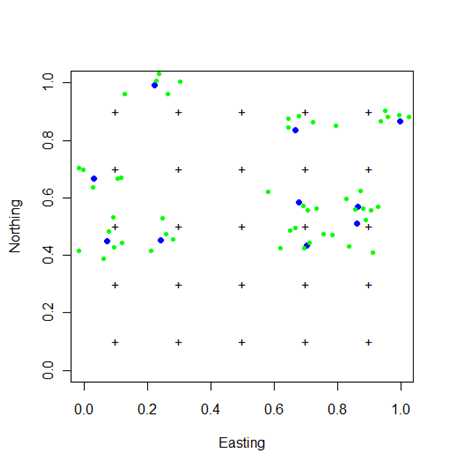
\includegraphics[height=3in]{northingeasting}
\end{center}
\caption{Needs a caption. Make this larger?}
\label{fig.Rcommands}
\end{figure}

\section{Lions and Tigers and Bears, oh my:  Genesis of
Spatial capture-recapture data}

A diverse number of methods and devices exist for producing individual
encounter history data with auxiliary spatial information about
individual locations. Historically, physical ``trap'' have been widely
used to sample animal populations. These include live traps, leg-hold
traps, mist nets, pitfall traps and many other types of
devices. Although these are still widely used, huge advances have been
made in developing new methodologies for obtaining encounter history
data non-invasively.

\subsection{Camera trapping}

Considerable recent work has gone into the development of
camera-trapping methodologies. For a historical overview of this
method see \citet{kays_etal:2008, kucera_barrett:2011}.  Several
recent synthetic works have been published including
\citet{nichols_karanth:2002}, and an edited volume by
\citet{oconnell_etal:2010} devoted solely to camera trapping concepts
and methods. As a method for estimating abundance some of the earliest
work that relates to the use of camera trapping data in
capture-recapture models originates from Karanth and colleagues
\citep{karanth:1995, karanth_nichols:1998, karanth_nichols:2000}. In
studies that use camera trapping, cameras are situated along trails or
at baited stations and individual animals are photographed and
subsequently identified either manually by a guy sitting around
matching pictures, or sometimes now using computational
methods. Camera trapping methods are widely used for species that have
stripe or spotting patterns that are unique. As such, the method is
now widely applied to tigers \citep{karanth:1995,
  karanth_nichols:1998}, ocelots
\citep{trolle_kery:2003,trolle_kery:2005}, leopards
\citep{balme_etal:2010}, and many other cat species. Camera traps are
also used for other species such as wolverines
\citep{magoun_etal:2011}, and even species that are less easy to
identify uniquely such as mountain lions and coyotes
(e.g. \citet{kelly_etal:2008}.  We note that even for species that are
not readily identified by pelage patterns, it is possibly to use
camera traps in conjunction with spatial capture-recapture models to
estimate density, if an initial sample of individuals can be collared
or tagged in some way so that subsequent encounter by camera-traps can
yield individual information. In this way, the probability of
encounter can be estimated from the camera traps based on the
pre-marked individuals, and this is applied to the frequencies of
unmarked individuals to estimate density.


\begin{figure}
\begin{center}
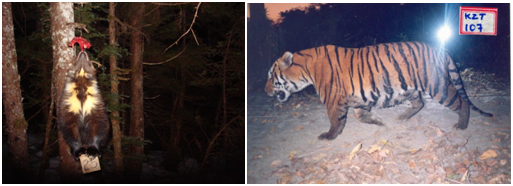
\includegraphics[width=5in]{wolverinetiger}
\end{center}
\caption{Wolverine in camera trap from A. Magoun (left). Picture of Tiger in
  camera trap from U. Karanth (right)}
\label{fig.wolverinetiger}
\end{figure}

\subsection{DNA Sampling}

Recent technological advances in the extraction and analysis of
genetic information have made a huge positive impact on studying
animal populations. DNA obtained from hair, blood or scat is now
routinely used to obtain individual identity and encounter history
information about individuals \citep{taberlet_bouvent:1992,
  woods_etal:1999, mills_etal:2000, schwartz_monfort:2008}.  A common
method is based on the use of ``hair snares'' (Fig. \ref{fig.bearcat})
which are widely used to study bear populations
\citep{woods_etal:1999, gardner_etal:2010, garshelis_etal:2006,
  kendall_etal:2009}.  A sample of hair is obtained as individuals
pass under or around barbed-wire (or other physical mechanism) to take
bait. Hair snares have also been used to sample felid populations
\citep{garciaalaniz_etal:2010} and other species. DNA information can
also be extracted from urine and as a result DNA can be used to study
feline populations which are attracted to scent-sticks and deposit
urine which is subsequently analyzed in the lab
\citep{valiere_taberlet:2000, kery_etal:2010}.


\begin{figure}
\begin{center}
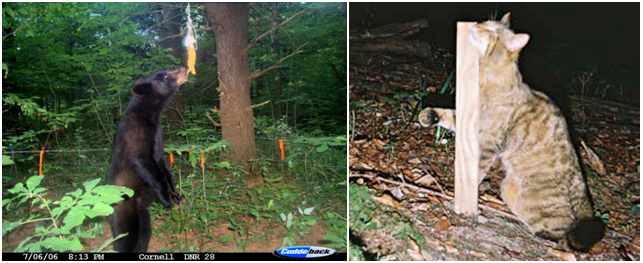
\includegraphics[width=5in]{bearcat}
\end{center}
\caption{Picture of hair snare. Bear (left). European wildcat
  (right). Pictures from??}
\label{fig.bearcat}
\end{figure}

\begin{figure}
\begin{center}
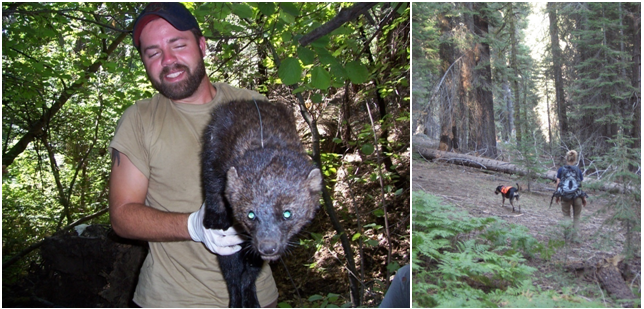
\includegraphics[width=5in]{beardog}
\end{center}
\caption{Guy holding fisher (left). Scat dog team working the ground
  (right). Pictures from Craig Thompson.}
\label{fig.fisherscatdog}
\end{figure}


There are other methods which don't fall into a nice clean taxonomy of
devices. DNA-based encounter histories can be obtained from scat
samples located along roads or trails or by specially trained dogs
\citep{mackay_etal:2008} searching space
(Fig. \ref{fig.fisherscatdog}). This method has been used in studies
of martens, fishers \citep{thompson_etal:inpress}, lynx, coyotes,
birds \citet{kery_etal:2010}, and many other species. We might search
space on foot and pick up individuals and physically mark them
somehow. This is pretty common in surveys that involve reptiles and
amphibians, e.g., we might walk transects through a forest and pick-up
box turtles \citep{hall_etal:1999} or search space for lizards
\citep{royle_young:2008} and also surveys designed to obtain animal
scat. These methods don't seem like normal capture-recapture in the
sense that the encounter of individuals is not associated with
specific locations of traps, but SCR models are equally relevant for
analysis of such data (see Chapter XY and Z).


\section{ Historical Context: A Brief Synopsis of the Literature}

Spatial capture-recapture is a relatively new methodological
development, at least with regard to formal estimation and
inference. However, the basic problems that motivate the need for
formal spatially-explicit models have been recognized for decades and
quite a large number of ideas have been proposed to deal with these
problems. The standard approach even now is to estimate $N$ using
conventional closed population models \citep{otis_etal:1978} and then
try to associate with this estimate some specific sampled area, say $A$,
the area which is contributing individuals to the population for which
$N$ is being estimated. The strategy is to define $A$ by placing a buffer
of say $W$ around the trap array or some polygon which encloses the trap
array. The historical context is well-stated by \citep{obrien:2011}
from which we draw this description:

\begin{quote}
  ``At its most simplistic, $A$ may be described by a concave polygon
  defined by connecting the outermost trap locations ($A_{tp}$; Mohr
  1947). This assumes that animals do not move from outside the
  bounded area to inside the area or vice versa. Unless the study is
  conducted on a small island or a physical barrier is erected in the
  study area to limit movement of animals, this assumption is unlikely
  to be true. More often, a boundary area of width $W$ ($A_{w}$) is added to
  the area defined by the polygon $A_{tp}$ to reflect the area beyond the
  limit of the traps that potentially is contributing animals to the
  abundance estimate (Otis et al. 1978). The sampled area, also known
  as the effective area, is then $A(W) = A_{tp} + A_{w}$. Calculation of the
  buffer strip width ($W$) is critical to the estimation of density and
  is problematic because there is no agreed upon method of estimating
  $W$. Solutions to this problem all involve ad hoc methods that date
  back to early attempts to estimate abundance and home ranges based
  on trapping grids 
  \citep[see][]{hayne:1949}. \citet{dice:1938} first drew attention
  to this problem in small mammal studies and recommended using
  one-half the diameter of an average home range. Other solutions have
  included use of inter-trap distances (Blair 1940; Burt 1943), mean
  movements among traps, maximum movements among traps (Holdenried
  1940, Hayne 1949), nested grids \citep{otis_etal:1978}, and assessment
  lines (Smith et al. 1971).''
\end{quote}

The idea of using 1/2 mean maximum distance moved
\citep{wilson_anderson:1985a} seems to be the standard approach even
today, presumably justified by Dice''s suggestion to use 1/2 the home
range diameter. Alternatively, some studies have used the full MMDM
(e.g. \citet{parmenter_etal:2003}). And, sometimes home range size is
estimated by telemetry \citep{karanth:1995}. This is usually combined
with an AIC-based selection from among the closed-population models in
\citet{otis_etal:1978} which most often suggests heterogeneity (Model
Mh).  Almost all of these early methods were motivated by studies of
small mammals using classical ``trapping grids'' but, more recently,
their popularity has increased with the advent of new technologies and
especially related to non-invasive sampling methods such as camera
trapping. In particular, the series of papers by Karanth and Nichols
\citep{karanth:1995, karanth_nichols:1998, karanth_nichols:2002} 
has led to fairly widespread adoption of these ideas.

\subsection{Seems like a subsection should be here}

Some of the heuristic ideas based on buffer strips do have some
technical justification in the sense of estimating parameters of an
underlying movement model from observed movements. For example, if we
let $x$ be a random variable indicating movement outcomes of an
individual about its  home range center, and suppose that $x$ has pdf
$g(x)$ then we can understand properties of MMDM by studying the
properties of the sample order statistics, as the maximum distance
moved is the sample range based on a sample of observations of
individual locations. As an illustration, imagine a 1-dimensional
system where individuals have a home range that amounts to a line
segment. Then suppose that individual movements are $\mbox{uniform}(0,A)$. It
can be shown that the sampling distribution of the sample range, R,
scaled by $A$, say $R/A$ has a beta distribution, $\mbox{beta}(n-1,2)$ 
\citep[][p. 235]{casella_berger:2002}
and thus the diameter of the home range, i.e. $A$, is
estimated (biasedly) by$ R/( (n-1)/(n+1) )$. For large $n$ we could then
say that the sample range, i.e., ''maximum distance moved'' seems like a good estimator of home range diameter and, therefore, $R/2$ is an estimator of home-range radius.  

There are a number of technical issues that arise in attempting to use
such heuristics to justify the application in practice. For one, the
moments of the sample order statistics are strongly affected by sample
size, which is typically quite small (per individual encountered) and
thus, in general, are biased and estimated with variable precision
depending on sample size. For example, the expected value of MMDM is
$k(n)*A$ , i.e., the true home range diameter is related to observed
MMDM by some function of sample size, $k(n)$, that increases to 1. In
the case where the underlying movement model is uniform, $k(n) =
(n-1)/(n+1)$ (from above) which motivates a formula for ``adjusting''
observed MMDM for small sample size. We suspect that many such
formulae are obtainable depending on the assumed movement distribution
\citep[e.g., formula 6.16 in][]{obrien:2011}. We might also think about taking
the {\it maximum} (over individuals) of the maximum distance moved
because under the specific model considered here (iid uniform) then
all individuals have the same home range radius. This increases our
sample size ($n$) and thus the observed sample range should be more
accurate. Another issue of somewhat more importance (and less easy to
rectify) is that the {\it observation} of movement outcomes is biased
by the locations of traps. We cannot observe movements ``off the
trapping grid'' (or between traps) and thus our observed movements
will generally be smaller than expected under any particular model
(the uniform in this case). Moreover, the trap spacing also induces a
discreteness to the movements that causes a further level of
approximation based on hypothetical movement
distributions. Nevertheless, formal analysis of `` buffering''
strategies based on sample order statistics under specific models for
movement does at least provide some heuristic support for specific
choices.  The interested reader should ponder the distribution of the
sample minimum, maximum and range under other distributions such as a
normal (and bivariate normal), exponential distribution and perhaps
others. In addition, contemplate the effect of censoring of movements
to some arbitrary limit ($B<A$) to mimic bias in observed movement
outcomes due to a finite trap grid.

\subsection{Some other subsection?}

The use of buffer strips is conventional and widespread due to the
heuristic appeal of that idea and its easy implementation, but other
conceptual approaches exist to address specific problems motivated by
the spatial context of capture-recapture data. D.R. Anderson came up
with the idea of the ``trapping web'' \citep{anderson_etal:1983} which
does not seem to have been widely adopted in practice.
% although there
%is a clear mathematical formalization to the trapping web design
%\citep{link_barker:1994}. 
One reason for this is 
the design is somewhat restrictive in the sense that it requires
a large number of traps be organized in close proximity to one
another. Another intuitively appealing idea is that by
\citet{white_shenk:2000} who discuss ``correcting bias of grid
trapping estimates'' by recognizing that the basic problem is like
random temporary emigration \citep{kendall_etal:1999}  where individuals flip a coin with
probability $\phi$ to determine if they are ``available'' to be sampled or not.
White and Shenk's idea was to estimate $\phi$ from radio telemetry, as the
proportion of time an individual spends in the study area. They obtain
the estimated super-population size by using standard closed
population models and then obtain density by $\hat{D} =
\hat{N}\hat{\phi}/A$ where $A$ is the nominal area of the trapping array
(e.g., minimum convex hull).  A problem with this approach is that 
individuals
that were radio collared represent a biased sample i.e.,
you fundamentally have to sample individuals randomly from the
population {\it in proportion to their exposure to sampling}
 and that seems practically impossible to accomplish.
%any better for radio collaring than you can for the basic
%capture-recapture study itself.  
That said, the temporary emigration
analogy is a good heuristic for understanding SCR models and has a
precise technical relevance to certain models.

Another very interesting idea is that of using some summary of
``average location'' as an individual covariate in standard
capture-recapture models. \citet{boulanger_mclellan:2001} use
distance-to-edge (DTE) as a covariate in the Huggins-Alho type of
model. \citet{ivan:2012} uses this approach in conjunction with an
adjustment to the estimated N obtained by estimating the proportion of
time individuals are ``on the area formally covered by the grid''
using radio telemetry.  We do not dwell too much on these different
variations but we do note that the use of DTE as an individual
covariate amounts to some kind of intermediate model between simple
closed population models and fully spatial capture-recapture models,
which we address directly in Chapter 3. We note that no adjustment
based on telemetry information is necessary if one were simply to
place a prior distribution on the individual covariate (which is not
to say that telemetry data isn't useful, just that the same objective
can be achieved without telemetry data).

While these procedures are all heuristically appealing, they are also
essentially ad hoc in the sense that the underlying model remains
unspecified or at least imprecisely characterized and so there is
little or no basis for modifying, extending or generalizing the
methods. These methods are distinctly {\it not} model-based procedures
even though they might well be heuristically appealing under specific
movement models. Despite this, there seems to be an enormous amount of
literature developing, evaluating and ``validating'' these literally
dozens of heuristic ideas that solve specific problems, as well as
various related tweeks and tunings of them and really it hasn't led to
any substantive breakthroughs that are sufficiently general or
theoretically rigorous.


\subsection{The modern age}

\citet{efford:2004} was the first to formalize an explicit model for
spatial capture-recapture problems in the context of trapping arrays.
He adopted a Poisson point process model to describe the distribution
of individuals and then what is essentially a distance sampling
formulation of the observation model which describes the probability
of detection as a function of individual location, regarded as a
latent variable governed by the point process model. While earlier
(and contemporary) methods of estimating density from trap arrays have
been ad hoc in the sense of lacking a formal description of the
spatial model, Efford achieved a formalization of the model, but
adopted a more or less ad hoc framework for inference under that
spatial model using a simulation based method known as inverse
prediction.

Recently, there has been a flurry of effort devoted to formalizing
inference under this model-based framework for the analysis of spatial
capture-recapture data. There are two distinct lines of work which
adopt the model-based formulation in terms of the underlying point
process but differ primarily by the manner in which inference is
achieved. One approach is a classical inference approach based on
likelihood \citep{borchers_efford:2008}, and the other adopts a
Bayesian framework for inference. To motivate the origins and
relevance of these approaches, we note that, fundamentally, spatial
capture-recapture models are related to classical ``individual
covariate'' models (colloquially referred to as Huggins-Alho 
models) in capture-recapture \citep{huggins:1989, alho:1990}.
In particular, individual covariate models 
are based on a logit model where the
individual covariate is observed, whereas it is unobserved in SCR
models. To accommodate that, a prior distribution for the individual
covariate is required. In essence then, SCR models are similar to a
fully model-based formulation of classical HA models (see
\citet{royle:2009}). A classical argument in favor of the HA model is
that it ``doesn't require assumptions about the covariate'' but the
assumption is explicit in capture-recapture models and thus it is
natural to attack inference based on the ``joint likelihood''
\citep{borchers_etal:2002}. This has proven necessary in certain other
classes of individual covariate models in which natural models arise
for the individual covariate, such as time-varying individual
covariates \citep{bonner_schwarz:2006}, or covariates with measurement
error (e.g., distance sampling; see
\citet[][ch. 7]{royle_dorazio:2008}). 
The model-based formulation is easily adapted to standard
individual covariate models as well \citep{royle:2008}. Throughout
this book we rely heavily on Bayesian inference of the joint
likelihood, using the formulation based on data-augmentation
\citep{royle_etal:2007, royle_young:2008, royle:2009} though we also
discuss the development of likelihood-based inference in chapter 5 and
apply those methods in some cases.


\section{ A Motivating Example }
 
We confront some of the issues that motivate the need for spatial
capture-recapture models by considering analysis of data from a study
design to estimate black bear abundance Fort Drum Military
Installation in upstate New York (see Ch. 3 for more details). The
specific data used here are encounter histories on 47 individuals
obtained from an array of 38 baited ``hair snares'' during June and
July 2006. The study area and locations of the 38 hair snares are
shown in Fig. \ref{fig.hairsnares}.  Barbed wire traps (see
Fig. \ref{fig.bearcat}) were baited and checked for hair samples each
week for eight weeks.  Analysis of these data appears in
\citet{gardner_etal:2010} and we use the data in a number of analyses
in later chapters.

\begin{figure}
\begin{center}
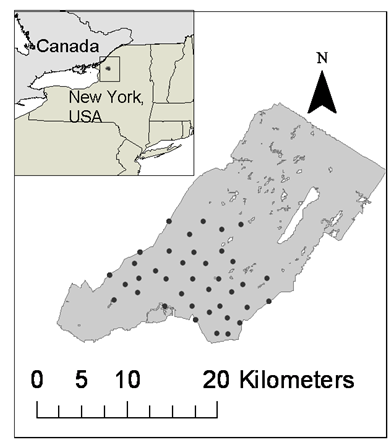
\includegraphics[height=3in]{hairsnares}
\end{center}
\caption{Locations of black bear hair snares on Fort Drum.}
\label{fig.hairsnares}
\end{figure}

We regarded this data set as a standard capture-recapture data set -
an encounter history matrix with 47 rows and 8 columns, where each
entries $y_{ik}=1$ if individual $i$ was captured in sample $k$ and
$y_{ij}=0$ otherwise. There is a standard closed population model,
colloquially referred to as ``Model M0'' (see Ch. 3), which assumes
that encounter probability $p$ is constant for all individuals and
sample periods.  We fitted Model M0 to the Fort Drum data using
traditional likelihood methods, yielding the maximum likelihood
estimate (MLE) of $\hat{N} = 49.19$ with an asymptotic standard error
(SE) of $1.9$.

The key issue in using closed population models with such data is how
on earth do we interpret this estimate of $N=49.19$ bears? Does it
represent the entire population of Fort Drum? Certainly not! Should we
assert that it applies to the southern half of Fort Drum below some
arbitrary line? Surely bears move on and off of Fort Drum without
regard to hypothetical boundaries. Without additional information
there is simply no way of converting this estimate of $N$ to density,
and hence it is really not meaningful biologically. To resolve this
problem, we will adopt the customary approach of converting $N$ to $D$
by buffering the convex hull around the trap array. The convex hull
has area $157.135 km^2$. We follow \citet{bales_etal:2005} in
buffering the convex hull of the trap array by the radius of the mean
female home range size. The mean female home range radius was
estimated \citep{wegan:2008} for our study region to be $2.19$ km, and
the area of the convex hull buffered by $2.19$ km is $277.01$ km$^2$. (R
commands to compute the convex hull, buffer it, and compute the area
are given in the Online Supplement).  Hence, the estimated density
here is approximately $0.178$ bears/km$^2$ for an estimated population
size obtained using Model M0.  We could assert that the problem has
been solved, go home, and have a beer.  But then, on the other hand,
maybe we should question this estimated home range radius from
\citep{wegan:2008} and, instead, rely on a buffer width based on
one-half MMDM estimated from the data as is more customary
\citep{dice:1938}. In that case the buffer width is $1.19$ km, and the
resulting estimated density is increased to $0.225$ bears/ha$^2$ about
27 \% larger.  On the other hand we might decide to use the full MMDM
(REF XYZ) which is $2.37$ km, pretty close to the telemetry-based estimate
and therefore providing a similar estimate of density ($0.171$ bears/ha$^2$.

In thinking about the use of model M0, we might naturally question
some of the basic assumptions that go into that model. The obvious one
to question is that which declares that $p$ is constant. One obvious
source of variation in $p$ is variation {\it among individuals}. We
expect that individuals may have more or less exposure to trapping due
to their location relative to traps. This has led many to consider
capture-recapture models that allow for individual heterogeneity in
$p$. Such models have the colloquial name of ``Model Mh.''
We fitted this model (see ch. 3 for details) to the Fort Drum data
using each of the 3 buffer widths previously described (telemetry, 1/2
MMDM and MMDM), producing the estimates reported in Table
\ref{tab.fdests}.

So what do we have here?  Our density estimates span quite a range
from $0.17$ to $0.43$ bears/km$^2$ depending on which estimator of $N$ we use and
what buffer strip we apply. Should we feel strongly about one or the other?
AIC favors model Mh by more than 30 units, but which buffer should we
prefer?  
%Moreover, we could find more variations of 
%model Mh to choose among, but see \citep{link:2003}. 
How do we characterize uncertainty of the buffer ``estimate''?  And,
in what sense is the
buffer even an estimate of something? What is it an estimate of? Who
knows?  Other issues we can't address: trap-specific covariates.
In summary, there's not a compelling solution to be derived from
this ``estimate $N$ conjure up a buffer'' approach. 

\begin{table}[ht]
\centering
\caption{Table on estimates of D for the Fort Drum data
using M0 and Mh and different buffers.}
\begin{tabular}{ll|cc} 
\hline
model & buffer &  $\hat{D}$ & SE \\ \hline
M0   & telemetry &  0.178 & 0.178 \\
M0    & MMDM     &  0.171 & 0.171\\
M0   & 1/2 MMDM  &  0.225 & 0.225\\
Mh(ln) & telemetry &0.341 & 0.144\\
Mh(ln) & MMDM    &  0.327 & 0.138\\
Mh(ln) & 1/2 MMDM & 0.432 & 0.183\\
\end{tabular}
\label{tab.fdests}
\end{table}

\section{Extension of Closed Population Models}

The deficiency with classical closed population models is that they
have no spatial context. $N$ is just an integer parameter that applies
equally well to some population in a computer, estimating the number
of unique words in a book, or a bucket full of goldfish.  The question
of {\it where} the $N$ items belong is central both to interpretation
of data and estimates from all capture-recapture studies and, in fact,
to the construction of spatial capture-recapture models considered in
this book.  Surely it must matter whether the $N$ items exist 
in a book, or a goldfish bowl, or a landscape patch!

Thus, the essential problem is that classical closed population models
are too simple - they ignore the spatial attribution of traps and
encounter events, movement and variability in exposure of individuals
to trap proximity, and they do not yield estimates {\it density}.
These are not problems per se but rather features (features
not bugs!) of this overly-simple class of models, and they 
should be addressed formally by the development of
more general models.  Spatial capture-recapture models are
statistical and mathematical models that extend non-spatial
``ordinary'' capture-recapture models to accommodate the spatial
structure inherent in sampling animal populations - i.e., trap
locations, individual locations, and individual use of space.

The solution to the various issues that arise in the application of
ordinary capture-recapture models is to extend the closed population
model so that $N$ becomes spatially explicit.  A natural way is to
define a point process \citep{efford:2004} that describes how
individuals are organized in space and that, when points are
aggregated over space, the value $N$ is derived in a meaningful way.
Thus, in this book, we adopt the view that the locations of the N
individuals in the population are a {\it realization of a spatial
  point process}.


\subsection{Abundance as the Aggregation of a Point Process}

Spatial point process models represent a major methodological theme in
spatial statistics \citep[][ch. xyz]{cressie:1992} and they are
widely applied as models for many ecological phenomena 
\citep{stoyan_penttinen:2000,illian:2008}. Point process models apply to
situations in which the random variable in question represents the
locations of events or objects: trees in a forest, weeds in a field,
bird nests, etc.  As such, it seems natural to describe the
organization of individuals in space using point process models. 

One
of the key features of SCR models is that the point locations are
latent, or unobserved, and we only obtain imperfect information about
the point locations by observing individuals at trap or observation
locations.  Thus, the realized locations of individuals represent a
type of ``thinned'' point process, where the thinning mechanism is not
random but, rather, biased by the observation mechanism.  It is
natural to think about the observed point process as some kind of a
compound or aggregate point process with a set of ``parent'' nodes
being the locations of individuals and the observed locations as
``offspring'' - i.e., a Poisson cluster process (PCP). In that
context, density estimation is analogous to estimating the number of
parents in the PCP \citep{chandler_royle:2012}. Other types of point
process models for the realized locations have direct relevance to SCR
models (See \citet{chandler_royle:2012}, discussed in chapter XYZ).

In the context of SCR models, we suppose there is a point on the
landscape that we'll think of as a home range center or, if this is
unappealing, we can think of it as the centroid of an individual's
activities during the time of sampling. In general, this point is
unknown for any individual but if we could track an individual over
time and take many observations then we could perhaps get a good idea
of where that point is.  We'll think of the collection of these points
as defining the spatial distribution of individuals in the
population. Most of the recent developments in modeling and inference
from spatial encounter history data, including most methods discussed
in this book, are predicated on the view that individuals are
organized in space according to a relatively simple point process
model. More specifically, we assume that the collection of individual
activity centers are ``iid'' random variables distributed uniformly
over some region. This is consistent with the assumption that the
activity centers represent the realization of a Poisson point process
or, if the total number of activity centers if fixed, then this is
usually referred to as a binomial point process.

We use the terms home range or activity center interchangeably. The
term ``home range center'' suggests that models are only relevant to
animals that exhibit such behavior of establishing home ranges or
territories and since not all species do that, perhaps the
construction of SCR models based on this idea is flawed. This isn't
really true -- the notion of a home range center is just a conceptual
device and we don't view this concept as being strictly consistent
with classical notions of animal territories but rather our view is
that a territory is inherently dynamic, temporally and thus also a
transient quantity - where the animal lived during the period of
study.  Whether or not individuals of a species establish home ranges
is therefore irrelevant - once a precise time period is defined,
individuals certainly must occupy distinct regions in space. In other
words, the definition of ``home range center'' is predicated, in a
sense, on the specification of a time period over which individuals
are studied. A term that might be less offensive than ``home range
center'' is ``centroid of space usage (CSU)'' which should not
conflict directly with preconceived understandings and interpretations
of home range\footnote{Utilization distribution is the same thing
  I guess?}.


\subsection{The state-space}

If we let ${\bf s}_{i}; i=1,2,\ldots,N$ be the locations of individual
activity centers, then the question ``what are the possible values of
${\bf s}$?'' needs to be addressed because the individual ${\bf
  s}_{i}$ are {\it unknown}. As a technical matter, we will regard
them as random effects and thus in order to apply standard methods of
statistical inference we need to provide a distribution for these
random effects.  In the context of the point process model, the
possible values of the point locations referred to as the
``state-space'' of the point process and this is some region or set of
points which we will denote by ${\cal S}$. In the relevant context,
${\cal S}$ is a region within which points are located - essentially a
prior distribution for s[i] (or, equivalently, the random effects
distribution). In the context of animal studies as a description of
where individuals that could be captured are located it encloses our
study area -- the region within which we might have located traps or
detection devices.  The state-space of the point process should
accommodate all individuals that could have been captured in the study
area.

In the practical application of SCR models, in most cases estimates of
density will be relatively insensitive to choice of state-space (see
Section XYZ) unless there are meaningful features to the state-space
which should be accommodated. For example, if the region within which
traps are located contains a coastline or a huge body of water then
clipping that out of the state-space will typically have a large
effect on density. This should be expected because, insofar as the
state-space serves as a prior distribution on the latent variables
${\bf s}_{i}$ then, {\it the state-space is very much a
  component of the model. } We discuss choosing the state-space in
Chapter 4.

When the underlying point process is well-defined, including a precise
definition of the state-space, this in turn induces a precise
definition of the parameter N ``population size'' as the number of
individual activity centers located within the prescribed state-space.
A deficiency with some classical methods of ``adjustment'' is they
attempted to prescribe something like a state-space - a ``sampled
area'' - except absent any precise linkage of individuals with the
state-space. SCR models formalize the linkage between individuals and
space and, in doing so, provide an explicit definition of $N$
associated with 
a well-defined spatial region, and hence
density. In a sense, the whole idea of SCR models is that by defining
this point process and its state-space ${\cal S}$, this gives context and
meaning to $N$ which can be estimated directly for that specific
state-space. Thus, it is fixing ${\cal S}$ that resolves the problem of
``unknown area'' that was addressed previously (Section XXXX). But the
existence of an explicit state-space ${\cal S}$ is kind of beside the
point -- ${\cal S}$ is really not always terribly important
itself. Instead, as soon as you give the latent variables ${\bf s}$ a
place to live, then you achieve spatial explicitness of the model
which is our primary objective.





\section{Hierarchical Models and Inference}

The term hierarchical modeling (or hierarchical model) has become
something of a buzzword over the last decade with hundreds of papers
published in ecological journals using that term.
So then, what exactly is a hierarchical
model, anyhow? Obviously, this term stems from the root ``hierarchy''
which means:

\vspace{.1in}

{\flushleft
Definition: {\it hierarchy} (noun) -- a series of ordered groupings of people or things within a system; 
}

\vspace{.1in}

In the case of a hierarchical model (hierarchical being the adjective
form of hierarchy), the ``things'' are probability distributions, and
they are ordered according to their conditional probability structure.
Thus, a hierarchical model is {\it an ordered series of models,
  ordered by their conditional probability structure}.  

If we declare
that the random variable $y = $ \# of times an individual is
encountered in a trap out of $T=10$ days has a binomial(10, p)
distribution then this is but a single model and, thus, not a
hierarchical model. If, however, we declare that 
\[
y \sim Bin(10,p)
\]
{\it and} 
\[ 
p \sim beta(1,1)
\] 
then this is kind of a cheap pedestrian
hierarchical model according to our definition although it is barely
more interesting than the previous non-hierarchical model.  

On the
other hand, suppose we have a collection of observations $y_{i}$ for
individuals $i=1,2,...,N$ and we declare 
\[
y_{i} \sim Bin(T, p_{i})
\]
 and
\[
p_{i}\sim beta(\mu, \tau)
\] 
then we have a more interesting
hierarchical model, this being a specific version of ``Model Mh'' (see
ch. 3 and \citet{dorazio_royle:2003}).  

A canonical hierarchical model in ecology is this
elemental model of species occurrence or distribution
\citep{mackenzie_etal:2002, tyre_etal:2003, kery:2011}:
\[
y_{i}|z_{i} \sim \mbox{Bin}(K,z \,  p)
\]
\[
z_{i} \sim \mbox{Bern}(\psi)
\]
where  $y_{i} = $ observation of presence/absence at a site $i$ and
$z_{i} = $ occurrence status ($z_{i}=1$ if a species occurs at  site
$i$ and $z_{i}=0$ if not). 

With these examples, 
we expand on our definition of a hierarchical model as we will use it in this book:

\vspace{.1in}

{\flushleft Definition: {\it Hierarchical Model}: A model with
  explicit component models that describe variation in the data due to
  (spatial/temporal) variation in {\it ecological process}, and due to
  {\it imperfect observation} of the process.  
}


\subsection{Anatomy of a hierarchical model}

Interesting hierarchical models in ecology typically 
contain the following components:
\begin{itemize}
\item[{\bf 1.}] {\it Observations}, $y(s,t)$ -- ``data''
\item[{\bf 2.}] {\it Observation model} $[y|z,\theta_1]$
\item[{\bf 3.}] {\it State variable}, $z(s,t)$: outcome of ecological {\it process} of interest
\item[{\bf 4.}] {\it Process model}  $[z|\theta_2]$ 
\item[{\bf 5.}] {\it Parameters}, $\theta_1$, $\theta_2$, that govern
  the observation and state processes
\end{itemize}


\subsection{Models don't have political views!} 

Whereas hierarchical modeling is a conceptual and framework for
formulating models, the method of inference is independent of model
formulation. Hierarchical models can be analyzed by Bayesian and
non-Bayesian methods. A model is not Bayesian or frequentist -- what
you do to that model is Bayesian or frequentist!
\[
\bullet \mbox{"Hierarchical model"} \ne  \mbox{"Bayesian"}!!!
\]
Thus, analysis of hierarchical models is easily achieved using either
Bayesian or classical (likelihood, frequentist) methods. By
``analysis'' we mean any type of estimation, characterization of
uncertainty, prediction, model selection, or evaluation and we are not
dogmatic about our choice of inference methods. That said, we do
recognize a benefit of the Bayesian approach which is that it
emphasizes model construction and not the construction of
procedures. The Nobel prize\footnote{called something else besides
  Nobel, officially} winning econometrician Christopher Sims (Slides
from the Hotelling Lecture 6/29/2007 at Duke University - cite his
webpage) said it this way: ``Bayesian inference is a way of thinking,
not a basket of 'Methods''' Conversely, ecologistis that are subjected
to a classical statistical curriculum often have only a vague sense of
what the model is that any particular procedure is employing.  We
agree with Little \citet{little:2006} 
that there should be more emphasis on understanding statistical
modeling, and less emphasis on statistical methods.  Toss the ``basket
of methods'' out the window and learn how to model!



\subsection{Spatial Capture-Recapture models as hierarchical models}

Most models considered in this book describe the encounter of
individuals conditional on the ``activity center'' of the individual,
which is a latent variable (i.e., unobserved random effect).  The
collection of these latent variables represents the outcome of an
ecological process describing how individuals distribute themselves
over the landscape. Moreover, how individuals are encountered in traps
is, in some cases, the result of a model governing movement.  As such,
these models are examples of hierarchical models that contain formal
model components representing both ecological process and also the
observation of that process. In \citet{royle_dorazio:2008} such models
were labeled as ``explicit'' hierarchical models because the process
component of the model corresponds to an actual or real
physical/biological or ecological process - the distribution of
individuals in space and their movements.  This is as opposed to
hierarchical models in which the process is ``implicit'' - usually
represented by a spatially or temporally indexed random effect that is
only, at best, a surrogate for something of ecological relevance
(``time effects'', ``space effects'' etc.).

{\bf Characterization of SCR models here maybe?}


\section{Analysis of spatial capture-recapture models}

We rely strictly on principles and procedures of {\it parametric
  inference} in our analysis of hierarchical models in general and,
specifically, of spatial capture-recapture models. Parametric
inference is that in which we make explicit probability assumptions
about how the data were generated. Inference procedures are then
developed under the assumption that the model is truth, because formal
parametric inference procedures that we understand the joint
probability distribution of everything that is a realization of a
random variable. There are two popular flavors of parametric
inference: {\bf Classical inference}: The joint probability distribution
of observations is the {\bf likelihood}. We maximize it to obtain MLEs
and do other fun things to it. We evaluate procedures by thinking
about what would happen over replicate realizations of data to which
our procedures are applied.  {\bf Bayesian inference} is based on the
posterior distribution, which is the joint probability distribution of
the data and also parameters and possibly other quantities including
latent variables or random effects.

Because SCR models contain a collection of latent variables - random
effects -- a natural framework for classical analysis of the models is
based on integrated likelihood \citep{laird_ware:1982,berger_etal:1999}. That is, while
the observation model is conceptualized conditional on the random
effects (the locations of individuals), classical inference is
formally based on the likelihood constructed from the {\it marginal}
probability distribution of the observations (i.e., {\it
  unconditional} on the random effect). The random effects are removed
from the conditional likelihood by integration (which is accomplished
numerically in spatial capture-recapture models). This approach to
inference has been formalized in the context of SCR models by
\citet{borchers_efford:2008, efford:2011}, and implemented for some
classes of models in the software package DENSITY \citep{efford:2004}
and the R package \mbox{\tt secr} \citep{efford:XYZ}.

Bayesian analysis is another natural framework for the analysis of
models containing latent variables or random effects.  Under this
approach, analysis of the model is based on Monte Carlo simulation
from the posterior distribution, which is the product of the
conditional likelihood, the distribution of the random effects, and
perhaps other distributions.  This approach was developed by
\citet{royle_young:2008}, and was motivated by work focused on
modeling individual effects in capture-recapture models. In
particular, a convenient reparameterization of individual covariate
models can be obtained using a method known as data augmentation
\citep{royle_etal:2007}, see \citet{royle:2008} for an application to
classical individual covariate models in \citet{royle:2008}. The close
similarity between individual covariate models and spatial
capture-recapture models, with the individual's activity center ${\bf
  s}$ being the individual covariate, led to the application of the
data augmentation method described by \citet{royle_young:2008} and subsequent papers. 

These two technical formulations (classical inference based on
integrated likelihood and Bayesian) both provide rigorous solutions to
the inference problems posed by spatial capture-recapture data.  As a
technical matter, \citet{borchers_efford:2008} and related work assume
a Poisson point process that is unconditional on $N$ whereas Royle and
Young (2008) and related work assume a binomial point process model
which is conditional on $N$.  More importantly, Borchers and Efford
develop the analysis in a way that is unconditional on the point
process (which is removed from the conditional likelihood by
integration).  Conversely, the analysis of \citet{royle_young:2008} is
conditional on the underlying point process. As a technical matter,
Bayesian analysis allows us to analyze the model that is conditional
on the underlying point process and will otherwise have more
flexibility - open populations, using telemetry data, etc.. as will be
demonstrated in later chapters.  More generally, integrated likelihood
for complex point process models may prove difficult, and so analysis
of the model that is conditional on the underlying point process will
prove to be more versatile and generalizable. We say this only
tentatively and throughout this book we are not exclusive in our views
of inference and use Bayesian and classical methods of inference
interchangeable and opportunistically in this book.

We don't want to get too much into the technical foundations of
Bayesian analysis because there are many good books now including
\citet{link_barker:2009}.  \citet{kery:2010, mccarthy:2007,
  king_etal:2009} and probably others by the time this book is
finished. That said, the basic ideas are worth highlighting for those
unfamiliar with the ideas.  But Bayesian analysis is introduced at a
level required to get through this book in Chapter 2.


\subsection{Implementing hierarchical models}

In our experience, students in ecology and even many established
scientists simply cannot separate what they need to do from how to do
it.  They cannot distinguish clearly (either conceptually or actually)
the difference between the model for their data, and the actual
procedure of how to estimate parameters of that model, or make
predictions - ie., how to do the calculations. Sometimes this issue
raises itself in an email from some hapless grad student wondering
``what is the right statistical test for this type of data?''  In a
sense it is this view that drives our approach to developing elements
of this book.

In contemporary statistical ecology, models and methods are sometimes
obscured by named procedures often that are completely uninformative,
the technical details of which hide in obscurity in some black boxes
such as MARK, PRESENCE, DISTANCE, etc., known only by the few
specialist experts in the field. While it is sometimes convenient to
refer to a type or class of models by a name (logistic regression or
even ``model Mh'') in order to emphasize a broad concept or
methodological area, this is only useful if the fundamental
statistical and mathematical structure underlying that name is
clear. As such, we try to focus on model development and keep the
model development distinct from how to combine our data with the model
to produce estimates and so forth. We talk a lot about hypothetical
data we wish we could observe - complete data sets - data sets as if
$N$ were known, etc.. We talk about the model in precise terms and
then break down various ways for analyzing the model either using
likelihood methods or Bayesian methods or some black-box that does one
or the other.

To fit models, we rely heavily on the various implementations of the
BUGS language including WinBUGS \citep{lunn_etal:2000}, JAGS (find
correct ref XXX) and OpenBUGS (find correct ref XXX). We really like
the BUGS language, not necessarily as a computational device for
fitting models but because the BUGS language really emphasizes
understanding of what the model is and fosters understanding how to
build models - as Kery says ``it frees the modeler in you.''  (direct
citation for this would be nice).  However, in addition to using the
BUGS language and its various implementations, we also develop our own
R code both for doing MCMC (some of which exists in the ``unmarked'' R
package) and also maximum likelihood, for which we also use the R
package SECR \citep{efford:2011}.


\subsection{This section has no home}

Of much more practical relevance is that many of the models described
here have a formulation that closely resembles generalized linear
models (GLMs) in which the individual activity centers appear as a
random effect \citep{royle_etal:2009, royle_gardner:2011}, similar to
generalized linear {\it mixed} models (GLMMs) which are pervasive in
the literature of many disciplines including ecology.  This actually
has, we think, some profound consequences both conceptually and
practically (in terms of implementation). For example, as a result,
SCR models should by conceptually accessible to practitioners with
some basic statistical understanding and experience.  And, we believe
that practitioners will have some flexibility in developing models
that fit their specific situation. Quite simply - given existing
software, it is easy for practitioners to specify models, even if they
lack the technical know-how to fit those models. As said by Marc Kery
(exact REF XXX) - in the context of his WinBUGS book - the BUGS
language ``frees the modeler in you'' (this quote is maybe out of
place a little bit).



\section{Characterization of SCR models}

For the purposes of this book, an SCR model is any ``individual
encounter model'' (not just ``capture-recapture''!) where auxiliary
spatial information is also obtained. To be more precise we could as
well use the term ``Spatial capture and/or recapture'' but that is
slightly unwieldy and, besides, it also abbreviates to SCR. The class
of SCR models includes traditional capture-recapture models with
auxiliary spatial information. However, we will see that some SCR
models do not involve ``recapture'' (e.g., distance sampling) and,
indeed, some don't even involve ``capture'' or even unique
identification of individuals! We discuss such models in later
chapters of this book.

Conceptually SCR models involve a collection of random
variables, ${\bf s}$, ${\bf u}$ and $y$ where ${\bf s}$ are the
activity or home range centers, ${\bf u}$ is the location of the
individual at the time of sampling (i.e., where the observer records
the animal) which we think of as realizations from some movement
model, and $y$ is the ``response variable'' - what the observer
records. E.g., $y=1$ means ``detected'' and $y=0$ means ``not
detected'' but many other types of responses are possible.
A broad class of models for estimating density are unified by a
hierarchical model involving explicit models for
animal home range centers ${\bf s}$, movement outcomes ${\bf u}$, and
encounter data $y$.  In some cases, we don't observe $y$ but rather
summaries of $y$, say $n(y)$, yet it might be convenient in such cases
to retain an explicit focus on $y$ in terms of model construction.
We thus introduce a sequence of models - a hierarchical model -
to relate these random variables and it goes something like this:
{\small 
\begin{verbatim}
# NEED A graphic made out of this somehow
# possibly a Directed Acyclic Graph with some parameters, 
# Fixed nodes, and stochastic nodes, might look cool. 

Home range center    movement model   observation model  [data summarization]
   g(s)                  h(u|s)            f(y|u)	        n(y)
\end{verbatim}
}
Thus, models covered in this book all have distinct
characteristics related to the following decomposition as a
hierarchical model:
\[
f(y|{\bf u})h({\bf u}|{\bf s})g({\bf s}).
\]

Every model we talk about in this book has either all of these
components or a subset of them. Examples
of such models are:
\begin{enumerate}
\item[$\bullet$] Classical distance sampling
\item[$\bullet$] Spatial capture-recapture models with fixed arrays of traps
  \citep{efford:2004, borchers_efford:2008, royle_etal:2009,
    royle_etal:2009, gardner_etal:2010}
\item[$\bullet$] Search-encounter models \citep{royle_young:2008, royle_etal:2011}.
\item[$\bullet$] Capture-recapture distance-sampling \citep{borchers_etal:1998}.
\end{enumerate}
In some classes of models, components for ${\bf u}$ and ${\bf s}$ will be confounded.
e.g., if ${\bf s}$ are uniform in space and ${\bf u}$ is
a random draw from some distribution centered at ${\bf s}$, then we might as
well define ${\bf u}^{*}=\Pr({\bf u})=\int_{s} [{\bf u}|{\bf s}][{\bf
  s}]ds$ which will itself by uniform
for reasonable choices of $[{\bf u}|{\bf s}]$.  Some examples
of typical spatial capture-recapture models include:
How these various model components are manifest in specific cases is
described as follows:
\begin{itemize}
\item[1.] {\bf Distance sampling -- } The last 2 stages of the hierarchy
  are confounded (implicitly) and so analysis is based on the model
  $[y|u*] [u*]$. The ``process model'' is that of ``uniformity'': ${\bf u}^{*}
  \sim Unif({\cal S})$. Sometimes it is argued that distance sampling
  estimators are ``pooling robust'' which is a way of saying they are
  (or may be)
  relatively insensitive to this assumption. That may be true, but the
  construction of distance sampling estimators makes explicit the
  uniformity assumption as a mathematical fact.

\item[2.] {\bf Spatial capture-recapture model with a fixed array of traps} --
SCR models appear to have little in common with distance sampling
because observations are made only at a pre-defined set of discrete
locations -- where traps are placed. However, the models are closely
related in terms of our hierarchical representation above\footnote{Really
they're kind of like point-count distance sampling where the identity
of individuals is preserved across point samples , and distance is a
latent variable. i.e., SCR-DS. I feel like this point should be
emphasized somehow. Here? Later?}
In SCR models based on fixed arrays, 
we cannot estimate both
$\Pr(y=1|{\bf u})$ and $\Pr({\bf u}|{\bf s})$ -- the probability  that
an individual ``moves to ${\bf u}$'' cannot be seperated from the
probability that it is detected given that it moves to ${\bf u}$,
because of the fact that the observation locations are fixed by
design.
Formally, such SCR models confound $[y|{\bf u}]$  with $[{\bf
  u}|{\bf s}]$ so that the observation model arises as:
\[
 [y|{\bf s}] = \int_{u} [y|{\bf u}][{\bf u}|{\bf s}] du
\]
This confounding happens because SCR sampling is spatially biased -
restricted to a fixed pre-determined set of locations. 

Conversely,
distance sampling confounds $[{\bf u}|{\bf s}][{\bf s}]$ because, essentially, there is
only a single realization of the encounter process.  

It is probably
reasonable to assume that $\Pr(y=1|{\bf u})=1$ or at least it is locally
constant for most devices (e.g., cameras, etc..), and thus the
detection model will have the interpretation in terms of movement (see
chapter XXX.YY).

\item[3.] {\bf Search-encounter models -- } What we call
  ``search-encounter'' models \citep{royle_etal:2011}
  are kind of a hybrid model - combining features of SCR models and
  features of distance sampling. Like distance sampling they allow for
  encounters in continuous space which provide direct observations
  from $[{\bf u}|{\bf s}]$.
Thus, the
  hierarchical model is fully identified.

\item[4.] {\bf Capture-recapture/distance-sampling -- } See
  \citet{borchers_etal:1998}. As with the search-encounter models the
full hierarchical model is identified:
$[y|{\bf u}][{\bf u}|{\bf s}][{\bf s}]$ but the quantities don't
really mean the same thing as before. 

To understand this, we expand the model to accommodate imperfect
measurements of ${\bf u}$. Let ${\bf u}_{obs}$ be an observation of
${\bf u}$ (i.e., made with error). A larger hiearchical model is this:
\[
[y|{\bf u}][{\bf u}_{obs}|{\bf u}][{\bf u}|{\bf s}][{\bf s}]
\]
If we make replicate ``instantaneous'' observations of location, then
information is provided about 
 $[{\bf u}_{obs}|{\bf u}]$ (i.e., measurement error). However, in a normal
 distance sampling application, with instantaneous sampling, we don't
 learn anything about $[{\bf u}|{\bf s}]$, 
in effect, we are again confounding $[{\bf u}|{\bf s}]$ and $[{\bf
  s}]$: ${\bf u}^{*} = \int_{s} [{\bf u}|{\bf s}][{\bf s}] ds$. So the CR-DS model focuses on:
\[
[y|{\bf u}^{*}][{\bf u}_{obs}|{\bf u}^{*}][{\bf u}^{*}].
\]
Structurally, this is the same basic model as the search-encounter
model notwithstanding (1) that it is usually talked about in terms of
repeated measures of distance instead of location and (2) the 2nd
component of the hierarchy is not movement (an ecological process) but
rather ``measurement error'' and (3) the third component is not a home
range center but rather a movement outcome (``instantaneous
location'').  Thus, while the models are structurally identically, the
meaning and interpretation of quantities are distinct. 

%These are
%mostly all semantic and conceptual distinctions which are easy to
%define in a convenient table:
%\begin{table}[ht]
%\centering
%\title{What things mean in each model.}
%\begin{tabular}{c|cc}
%           &   Search encounter models     &  CR-DS  \\  \hline
%  $\sigma$    &  movement       &   measurement error  \\
% ${\bf s}$ & activity center & instaneous location \\
%\end{tabular}
%\end{table}
\end{itemize}


\subsection{Other elements of SCR models}

There are other considerations to think about developing here.

\subsubsection{1. The state-space.}

 The state-space of the
underlying point process: is it continuous or discrete (e.g.,
polygons)?

\subsubsection{2. individual locations.}

Are the observation locations (of individuals) fixed
points or made in continuous space, or even polygons?

\subsubsection{3. spatial sampling.}

What is the nature of spatial sampling?
Statistically structured or unstructured
(haphazard or opportunistically). 

Broadly speaking we differentiate
between two situations: Sampling based on fixed arrays or sampling
based on ``search encounter'' methods. The former includes things like
camera traps, hair snares, mist nets and conventional traps. Fixed
arrays limit the observation location to pre-defined points, where
traps are located. Using such methods the model is a little simpler
because the ``movement process'' of individuals is confounded with the
``observation process''.
The 2nd type of model -- search encounter models -- typically
will allow locations in continuous space, possibly only restricted by
polygon boundaries \citep{royle_young:2008}. 
Search-encounter data
usually allow for the separate modeling and estimation of movement
model parameters from encounter model parameters but not always,
depending on whether replication of the sampling is done.  The
classical DS model with no replication (i.e., t=1) is a basic model
which confounds the two processes.

\subsubsection{4. observation model.}

Properties of the ``detection apparatus'' induce statistical
properties of the random variable $y$. Some typical ``observation
models'' include:
Bernoulli, binomial, Poisson,
multinomial. 


Depending on the type of device being considered, certain restrictions
on the observable variable are induced which suggest specific
probability models for the observable random variable. One type of a
device is what we think of as the classical ``camera trap'' and which
\citet{efford:2011} refers to as a ``proximity detector''. We can take
pictures of or detect any number of individuals and an individual can
be caught in any number of traps, and an arbitrary number of
times. Iid Bernoulli model is convenient but if you think the
re-encounters are valuable then you can have a frequency model.  Bear
hair snares are slightly different because you cannot differentiate
re-encounters.

The standard observation model that applies for ``single-catch''
\citep{efford_etal:2004} traps posits that individuals are encountered
in at most one trap per sample occasion and traps only hold one
individual.  Unfortunately we're really screwed in the single-catch
situation.

A ``multi-catch'' is like a mist-net or other things - individual is
captured and restrained but traps hold > 1 individual. In this case,
the observation model is a multinomial. Iid is assumed.  There are
many variations on all of these models and new models. E.g., Telemetry
data. Incidental observations of individuals.

\subsubsection{5. modeling distance}

An important part of the observation model of every SCR model is the
manner in which {\it distance} between individuals and observation
locations (``sampler'') enters into the model. 
This depends on whether the sampling is done at a point, along a line,
or uniformly over some polygon.

Observation location $x$ is a point.  We record individual location at
point $x$ or at some other location $u$. Distance is either $||x-s||$
or $||x-u||$.

Observation location is a ``line'':
(i) if we note point on line {\it and} $u$ then radial distance $||x - u||$
(ii) We don't observe point on line we might use ``closest distance''
(standar distance sampling)
(iii) we may or may not observe ${\bf u}$.
(iv) we might only record ${\bf u}$ but not the point on the line. In
that case we could use closest-distance or ``total hazard''.

More often, distance samplers approximate this with the closest linear
distance to the line, i.e., $min_{x} ||u-x||$.  Someone told me that
this has been found to work better in practice but clearly it is not the
correct description of the observation mechanism (when $x$ is available).
An alternative is to use the cumulative hazard (from Buckland and Hayes paper)
where we sum the hazard from the start of the line up to point $x$.



\section{Summary and Outlook}

Spatial capture-recapture models are an extension of ordinary
capture-recapture models to accommodate the spatial organization of
both individuals in a population and the observation mechanism (e.g.,
locations of traps).  They resolve problems which have been recognized
historically and for which various ad hoc solutions have been
suggested: heterogeneity in encounter probability due to the spatial
organization of individuals relative to traps and also that a
well-defined sample area does not exist in most studies, and thus
estimates of N using ordinary capture-recapture models cannot be
related directly to density.


\subsection{The Promise and Pitfalls of SCR models}

Ecological scientists study elements of ecological theory using
observational data that exhibits various biases relating to the
observation mechanisms employed. In the context of capture-recapture,
we observe individual encounter history data from which we can use SCR
models to infer where individual live, how they organize themselves in
space and move around in space and how they interact with other
individuals.  Moreover, SCR models show great promise in their ability
to integrate explicit ecological theories directly into the models so
that we can directly test hypotheses. For example, point process
models can be used to model inhibition, clustering or interactions
among individuals.

Thus, SCR models are capture-recapture models that enable ecologists
to explicitly integrate biological context and theory with encounter
history data, which is something that has always been the focus of
``open population'' models but never, until very recently, has been
considered formally in closed population models. We therefore believe
that SCR models will enable ecologists to test theories of space usage
and environmental effects, social behavior and other important
theories.


\subsection{Where to from here?}

In chapter 2 we provide the basic analysis tools to understand and
analyze SCR models - namely GLMs with random effects, and their
analysis in R and WinBUGS.  Because SCR models represent extensions of
basic closed population models, we cover ordinary closed population
models in chapter 3 wherein, along with chapter 4, we will see that
SCR models are a type of individual covariate model, which are
conceptual and technical intermediates between Model Mh and classical
individual covariate models.  In subsequent chapters we will cover a
bunch of different types of SCR models related to the type of
encounter process - e.g., type of trap - and also different
embellishments of the basic model structure as alluded to in section
XYZ above.  We will consider many different extensions of SCR models
to accommodate covariates on encounter probability, and density. We
also consider important practical extensions such as SCR for open
populations (Chapter xyz), combining SCR data with auxiliary
information from telemetry (chapter XYZ) and multiple encounter
methods (chapter XYZ).


\chapter{
Closed Population Models
}
\markboth{Chapter 3}{}
\label{chapt.intro}

% edited 12/12/2011 
% edited 12/13/2011

\vspace{.3in}

In this chapter we will consider ordinary capture-recapture (CR)
models for estimating population size in closed populations. We will
see that such models are closely related to binomial (or logistic)
regression type models. In fact, when $N$ is known, they are precisely
such models.  We consider some important extensions of ordinary closed
population models that accommodate various types of ``individual
effects'' --- either in the form of explicit covariates (sex, age,
body mass) or unstructured ``heterogeneity'' in the form of an
individual random effect. In general, these models are variations of
generalized linear or generalized linear mixed models (GLMMs).
Because of the paramount importance of this concept, we focus mainly
on fairly simple models in which the observations are individual
encounter frequencies, $y_{i}$ = the number of encounters of
individual $i$ out of $K$ replicate samples of the population which,
for the models we consider here, is the outcome of a binomial random
variable.  Along the way, we consider the spatial context of
capture-recapture data and models and demonstrate that density cannot
be formally estimated when spatial information is ignored. We also
review some of the informal methods of estimating density using CR
methods, and consider some of their limitations.  We will be exposed
to our first primitive spatial capture-recapture models which arise as
relatively minor variations of so-called ``individual covariate
models'' (of the \citet{huggins:1989} and \citet{alho:1990}
variety). In a sense, the point of this chapter is to establish that
linkage in a direct and concise manner beginning with the basic
``Model M0'' and extensions of that model to include individual
heterogeneity and also individual covariates. A special type of
individual covariate models is distance sampling, which could be
thought of as the most primitive spatial capture-recapture model.  In
later chapters we further develop and extend ideas introduced in this
chapter.

We emphasize Bayesian analysis of capture-recapture models and we
accomplish this using a method related to classical ``data
augmentation'' from the statistics literature
\citet[e.g.,][]{tanner_wong:XXXX}).  This is a general concept in
statistics but, in the context of capture-recapture models where $N$
is unknown, it has a consistent implementation across classes of
capture-recapture models and one that is really convenient from the
standpoint of doing MCMC \citep{royle_etal:2007}. We use data
augmentation throughout this book and thus emphasize its conceptual
and technical origins and demonstrate applications to closed
population models.  We refer the reader to
\citet[][ch. 6]{kery_schaub:2011} for an accessible and complimentary
development of ordinary closed population models.


\section{The Simplest Closed Population Model: Model M0}

We suppose that there exists a population of $N$ individuals which we
subject to repeated sampling, say over $K$ nights, where individuals
are captured, marked, and subsequently recaptured.  We suppose that
individual encounter histories are obtained, and these are of the form
of a sequence of 0's and 1's indicating capture $(y=1)$ or not $(y=0)$
during any sampling occasion (``sample'').  As an example, suppose
$K=5$ sampling occasions, then an individual captured during sample 2
and 3 but not otherwise would have an encounter history of the form
${\bf y}=(0,1,1,0,0)$. Thus, the observation ${\bf y}_{i}$ for each
individual $(i)$ is a vector having elements denoted by $y_{ik}$ for
$k=1,2,..,K$. Usually this is organized as a row of a matrix with
elements $y_{ik}$, see Table \ref{tab.3.1}.  Except where noted
explicitly, we suppose that observations are independent within
individuals and among individuals.  Formally, this allows us to say
that $y_{ik}$ are Bernoulli random variables and we may write $y_{ik}
\sim \mbox{Bern}(p)$.  Consequently, for this very simple model in
which $p$ is in fact constant, then we can declare that the individual
encounter frequencies (total captures), $y_{i} = \sum_{k} y_{ik}$,
have a binomial distribution based on a sample of size $K$. That is
\[
y_{i}  = \sum_{k} y_{ik} \sim \mbox{Bin}(p,K) 
\]
for every individual in the population. This is a remarkably simple
model that forms the cornerstone of almost all of classical
capture-recapture models, including most spatial capture-recapture
models discussed throughout this book.  Evidently, the basic
capture-recapture model structure is precisely a simplistic version of
a logistic-regression model with only an intercept term
($\mbox{logit}(p) = \mbox{constant}$).  To say that all
capture-recapture models are just logistic regressions is only
slightly inaccurate. In fact, we are proceeding here ``conditional on
$N$'', i.e., as if we knew $N$. In practice we don't, of course, and
that is kind of the point of capture-recapture models as estimating
$N$ is the central objective. But, by proceeding conditional on $N$,
we can specify a simple model and then deal with the fact that $N$ is
unknown using standard methods that you are already familiar with
(i.e., GLMs - see chapter 2).
\begin{table}
\centering
\caption{a capture-recapture data set with $n=6$ observed individuals
and $K=5$ samples.}
\begin{tabular}{r|ccccc|c}
&  \multicolumn{5}{c}{Sample occasion} &  \\ \hline
 indiv $i$ &  1 & 2 & 3 & 4 & 5 & $y_{i}$ \\ \hline
  1 &     1 & 0 & 0 & 1 & 0  & 2   \\
  2 &     0 & 1 & 0 & 0 & 1  & 2   \\
  3 &     1 & 0 & 0 & 1 & 0  & 2   \\
  4 &     1 & 0 & 1 & 0 & 1  & 3   \\
  5 &     0 & 1 & 0 & 0 & 0  & 1   \\
  $n=6$ & 1 & 0 & 0 & 0 & 0  & 1   \\ \hline
\end{tabular}
\label{tab.3.1}
\end{table}

Assuming individuals of the population are observed independently, the 
joint probability distribution of the observations is the product of 
$N$ binomials
\begin{eqnarray*}
  \Pr(y_1, \ldots, y_N | p) &=& \prod_{i=1}^N  \mathrm{Bin}(y_i | K, p) \\
   &=& \prod_{k=0}^K  \pi(k)^{n_k}
\end{eqnarray*}
where $\pi(k) = \mathrm{Bin}(k | K,p)$ and where $n_k = \sum_{i=1}^N
I(y_i = k)$ denotes the number of individuals captured $k$ times in
$K$ surveys. We emphasize that this is conditional on $N$, in which
case we get to observe the $y=0$ observations and the resulting data
are just $iid$ binomial counts. Because this is a binomial regression
model of the variety described in chapter 2, fitting this model using
a BUGS engine poses no difficulty.

The essential problem in capture-recapture, however, is that $N$ is
not known because the number of uncaptured/missing individuals (i.e.,
those in the zero cell that occur with probability $\pi(0)$) is
unknown.  Consequently, the observed capture frequencies $n_k$ are no
longer independent. Instead, their joint distribution is multinomial
(e.g., see \citet{illian_etal:2008} p XYZ):
\begin{equation}
\label{eq:multinomialForM0}
    n_1, n_2, \ldots, n_K \sim \mathrm{Multin}(N, \pi(1), \pi(2), \ldots, \pi(K))
\end{equation}
Note that in our notation the number of uncaptured/missing individuals is 
denoted by $n_0 = N - n$, where $n = \sum_{k=1}^K n_k$ denotes the total 
number of distinct individuals seen in the $K$ samples.

To fit the model in which $N$ is {\it unknown}, we can regard $N$ as a
parameter and maximize the multinomial likelihood directly.  While
direct likelihood analysis of the multinomial model is
straightforward, that does not prove to be too useful in practice
because we seldom are concerned with models for the aggregated
encounter history frequencies. In many instances, including for
spatial capture-recapture (SCR) models, we require a formulation of
the model that can accommodate individual level covariates which we
address subsequently in this chapter.



\subsection{The Spatial Context of Capture-Recapture}

A common assumption made is that of population ``closure'' which is
really just a colloquial way of saying (in part) the Bernoulli
assumptions stated explicitly above. In the biological context,
closure means, strictly, no additions or subtractions from the
population during study. This is manifest by the statement that the
encounters are independent and identically distributed (iid) Bernoulli
trials.  In practice, closure is usually interpreted by the manner in
which potential violations of that assumption arise. In particular,
two important elements of the closure assumption are ``demographic''
and ``geographic'' closure. If an individual dies then subsequent
values of $y_{ik}$ are clearly no longer Bernoulli trials with the
same parameter $p$. If there is no mortality or recruitment in the
population, then we say that demographic closure is
satisfied. Similarly, animals may emigrate or immigrate. If they do
not, then geographic closure is satisfied. Sometimes a distinction is
made between temporary and permanent emigration or immigration. That
is a relevant distinction in spatial capture-recapture models, because
SCR models explicitly accommodate ``temporary emigration'' of a
certain type, due to individuals moving about their home range. The
demographic closure assumption can also be relaxed using SCR models,
but we will save that discussion for chapter XYZ.



\subsection{Conditional likelihood}

We saw that a basic closed population model is a simple logistic
regression model if $N$ is known and, when $N$ is unknown, the model
is multinomial with index or sample size parameter $N$. This
multinomial model, being conditional on $N$, is sometimes referred to
as the ``joint likelihood'' the ``full likelihood'' or the
``unconditional likelihood'' (or model in place of likelihood). This
formulation differs from the so-called ``conditional likelihood''
approach in which the likelihood of the observed encounter histories
is devised conditional on the event that an individual is captured at
least once.  To construct this likelihood, we have to recognize that
individuals appear or not in the sample based on the value of the
random variable $y_{i}$, that is, we capture them if and only if
$y_{i}>0$.  The observation model is therefore based on $\Pr(y|y>0)$.
For the simple case of Model M0, the resulting conditional
distribution is a ``zero truncated'' binomial distribution which
accounts for the fact that we cannot observe the value $y=0$ in the
data set \citep[see][section XYZ]{royle_dorazio:2008}.  Both the
conditional or unconditional models are legitimate modes of analysis
in all capture-recapture types of studies, and they provide equally
valid descriptions of the data and for many practical purposes provide
equivalent inferences, at least in large sample sizes
\citep{sanathanan:1972}.

In this book we emphasize Bayesian analysis of capture-recapture
models using data augmentation (discussed subsequently), which
produces yet a third distinct formulation of capture recapture-models
based on the zero-{\it inflated} binomial distribution that we
describe in the next section.  Thus, there are 3 distinct formulations
of the model -- or models of analysis -- for analyzing all
capture-recapture models based on the (1) binomial model for the joint
or unconditional specification; (2) zero-truncated binomial that
arises ``conditional on $n$''; and (3) the zero-inflated binomial that
arises under data augmentation.  Each formulation has a distinct
complement of model parameters (shown in Table \ref{tab.3.modes} for
Model M0).


\begin{table}
\centering
\begin{tabular}{ccc}
Mode of analysis & parameters in model & statistical model \\ \hline
Joint likelihood                &	$p$, $N$	&	multinomial with index $N$\\
Conditional likelihood 		&	$p$	&	zero-truncated binomial \\
Data augmentation		&	$p$, $\psi$	&	zero-inflated binomial\\
\end{tabular}
\caption{Modes of analysis of capture-recapture models.}
\label{tab.3.modes}
\end{table}



\section{ Data Augmentation }

We consider a method of analyzing closed population models using data
augmentation (DA) which is useful for Bayesian analysis and, in
particular, analysis of models using the various BUGS engines and
other software.  Data augmentation is a general statistical concept
that is widely used in statistics in many different settings. The
classical reference is \citet{tanner_wong:1987} but see also
\citet{liu_wu:1999}.  Data augmentation can be adapted to provide a
very generic framework for Bayesian analysis of capture-recapture
models with unknown $N$. This idea was introduced for closed
populations by \citet{royle_etal:2007}, and has subsequently been
applied to a number of different contexts including individual
covariate models \citep{royle:2009}, open population models
\citep{royle_dorazio:2008,royle_dorazio:2010, gardner_etal:2010},
spatial capture-recapture models \citep{royle_young:2008,
  royle_etal:2010, gardner_etal:2009}, and many others.


Conceptually, data augmentation takes the data you wish you 
had - that is, the data set with $N$ rows - the known-$N$ data set - and 
embeds that data set into a larger data set having $M > N$ rows.
\footnote{ RC: Might be just me, but I find that formulation a little 
confusing... I think it's the 'data you wish you had because that's 
effectively data you don't have. I think it might be easier to grasp 
if this were explained with the data you do have - based on n. }
 It is always possible, in practice, to choose $M$ pretty easily for 
 a given problem and context. Then, under data augmentation, analysis 
 is focused on the ``augmented data set.'' That is, we analyze the bigger 
 data set - the one having $M$ rows - with an appropriate model that 
 accounts for the augmentation. Inference is focused directly on 
 estimating the proportion $\psi = E[N]/M$, instead of directly on $N$, 
 where $\psi$ is the ``data augmentation parameter.''



\subsection{DA links occupancy models and closed population models}

We provide a heuristic description of data augmentation based on the
close correspondence between so-called ``occupancy'' models and closed
population models following \citet{royle_dorazio:2008} sec. XYZ).

In occupancy models \citep{mackenzie_etal:2002, tyre_etal:2003} the
sampling situation is that $M$ sites, or patches, are sampled multiple
times to assess whether a species occurs at each site.  This yields
encounter data such as that illustrated in the left panel of Table
\ref{tab.3.occ}. The important problem is that a species may occur at
a site, but go undetected, yielding the ``all-zero'' encounter
histories which are observed. However, some of the all-zeros may well
correspond to sites where the species in fact {\it does not}
occur. Thus, while the zeros are observed, there are too many of them
and, in a sense, the inference problem is to allocate the zeros into
``structural'' (fixed) and ``sampling'' (or stochastic) zeros. More
formally, inference is focused on the parameter $\psi$, the
probability that a site is occupied.  In contrast, in classical closed
population studies, we observe a data set as in the middle panel of
Table \ref{tab.3.occ} where {\it no} zeros are observed. The inference
problem is, essentially, to estimate how many sampling zeros there are
- or should be - in a ``complete'' data set. The inference objective
(how many sampling zeros?) is precisely the same for both types of
problems if an upper limit $M$ is specified for the closed population
model. The only distinction being that, in occupancy models, $M$ is
set by design (i.e., the number of sites to visit) whereas a natural
choice of $M$ for capture-recapture models may not be
obvious. However, by assuming a uniform prior for $N$ on the integers
$[0,M]$, this upper bound is induced \citep{royle_etal:2007}. Then,
one can analyze capture-recapture models by adding $M-n$ all-zero
encounter histories to the data set and regarding the augmented data
set, essentially, as a site-occupancy data set.

Thus, the heuristic motivation of data augmentation is to fix the size
of the data set by adding {\it too many} all-zero encounter histories
to create the data set shown in the right panel of Table
\ref{tab.3.occ} - and then analyze the augmented data set using an
occupancy type model which includes both ``unoccupied sites'' as well
as ``occupied sites'' at which detections did not occur. We call these
$M-n$ all-zero histories ``potential individuals'' because they exist
to be recruited (in a non-biological sense) into the population, for
example during an analysis by MCMC.

To analyze the augmented data set, we recognize that it is a
zero-inflated version of the known-$N$ data set. That is, some of the
augmented all-zeros are sampling zeros (corresponding to actual
individuals that were missed) and some are ``structural'' zeros, which
do not correspond to individuals in the population. For a basic
closed-population model, the resulting likelihood under data
augmentation - that is, for the data set of size $M$ -- is a simple
zero-inflated binomial likelihood.  The zero-inflated binomial model
can be described ``hierarchically'', by introducing a set of binary
latent variables, $z_{1},z_{2},\ldots, z_{M}$, to indicate whether
each individual $i$ is ($z_i=1$) or is not ($z_i=0$) a member of the
population of $N$ individuals exposed to sampling. We assume that
$z_{i} \sim \mbox{Bern}(\psi)$ where $\psi$ is the probability that an
individual in the data set of size $M$ is a member of the sampled
population - in the sense that $1-\psi$ is the probability of
realizing a ``structural zero'' in the augmented data set.  The
zero-inflated binomial model which arises under data augmentation can
be formally expressed bythe following set of assumptions:

\begin{eqnarray*}
 y_{i}|{z_{i}=1} & \sim  &\mbox{Bin}(K, p) \\
 y_{i}|{z_{i}=0} & \sim &  \delta(0)  \\
 z_{i} & \stackrel{iid}{\sim} & \mbox{Bern}(\psi) \\
 \psi & \sim & \mathrm{Unif}(0,1) \\
 p & \sim & \mathrm{Unif}(0,1)
\end{eqnarray*}
for $i=1, \ldots, M$, where $\delta(0)$ is a point mass at $y=0$. 

We note that $N$ is no longer an explicit parameter of this
model. Instead, we estimate $\psi$ and functions of the latent
variables. In particular, under the assumptions of the zero-inflated
model, $z_{i} \stackrel{iid}{\sim} \mbox{Bern}(\psi)$; therefore, $N$
is a function of these latent variables:
 \[
 N = \sum_{i=1}^{M} z_{i}.
\]
Further, we note that the latent $z_i$ parameters can be removed from
the model by integration, in which case the joint probability of the
data is
\begin{eqnarray*}
  \Pr(y_1, \ldots, y_M | p, \psi) &=& \prod_{i=1}^M  \psi \mathrm{Bin}(y_i | K, p) +  I(y_i=0) (1-\psi)
\end{eqnarray*}
Which can be maximized directly to obtain the MLEs of the structural
parameters $\psi$ and $p$ or those of other more complex models
\citep[e.g., see][]{royle:2006}. We could estimate these parameters
and then use them to obtain an estimator of $N$ using the so-called
``Best unbiased predictor'' \citep[see][]{royle_dorazio:2011}.

\begin{table}
\centering
\caption{Hypothetical occupancy data set (left), capture-recapture data
 in standard form (center), and capture-recapture data augmented with
 all-zero capture histories (right). }
\begin{tabular}{cccc|cccc|cccc}
\hline
\multicolumn{4}{c}{Occupancy data}    &
\multicolumn{4}{c}{Capture-recapture} &
\multicolumn{4}{c}{Augmented C-R}     \\ \hline
site    & k=1 & k=2 & k=3 & ind & k=1 &k=2  & k=3 & ind & k=1 & k=2 & k=3           \\ \hline
1  & 0   & 1   & 0   & 1   & 0   & 1  & 0   & 1   & 0   & 1   & 0                   \\
2  & 1   & 0   & 1   & 2   & 1   & 0 & 1    & 2 & 1 & 0 & 1 \\
3  & 0   & 1   & 0   & .   & 0   & 1 & 0    & 3 & 1 & 0 & 1 \\
4  & 1   & 0   & 1   & .   & 1   & 0 & 1    & 4 & 1 & 0 & 1 \\
5  & 0   & 1   & 1   & .   & 0   & 1 & 1    & 5 & 1 & 0 & 1 \\
.  & 0   & 1   & 1   & .   & 0   & 1 & 1    & . & 0 & 1 & 1 \\
.  & 1   & 1   & 1   & .   & 1   & 1 & 1    & . & 0 & 1 & 1 \\
.  & 1   & 1   & 1   & .   & 1   & 1 & 1    & . & 1 & 1 & 1 \\
   & 1   & 1   & 1   & .   & 1   & 1 & 1    & . & 1 & 1 & 1 \\
n  & 1   & 1   & 1   & n   & 1   & 1 & 1    & n & 1 & 1 & 1 \\
.  & 0   & 0   & 0   &     &     &   &      & . & 0 & 0 & 0 \\
.  & 0   & 0   & 0   &     &     &   &      & . & 0 & 0 & 0 \\
   & 0   & 0   & 0   &     &     &   &      &   & 0 & 0 & 0 \\
   & 0   & 0   & 0   &     &     &   &      &   & 0 & 0 & 0 \\
   & 0   & 0   & 0   &     &     &   &      &   & 0 & 0 & 0 \\
   & 0   & 0   & 0   &     &     &   &      & N & 0 & 0 & 0 \\
.  & 0   & 0   & 0   &     &     &   &      & . & 0 & 0 & 0 \\
.  & 0   & 0   & 0   &     &     &   &      &   & 0 & 0 & 0 \\
M  & 0   & 0   & 0   &     &     &   &      & . & 0 & 0 & 0 \\
   &     &     &     &     &     &   &      & . & . & . & . \\
   &     &     &     &     &     &   &      & . & . & . & . \\
   &     &     &     &     &     &   &      & . & . & . & . \\
   &     &     &     &     &     &   &      & M & 0 & 0 & 0 \\
\end{tabular}
\label{tab.3.occ}
\end{table}


\subsection{Model $M_0$ in BUGS}

For model $M_0$ in which we can aggregate the encounter data to
individual-specific encounter frequencies, the augmented data are
given by the vector of frequencies $(y_{1}, \ldots, y_{n}, 0, 0,
\ldots, 0)$. The zero-inflated model of the augmented data combines
the model of the latent variables, $z_{i} \sim \mbox{Bern}(\psi)$ with
the conditional-on-$z$ binomial model:
\begin{eqnarray*}
y_{i} | z_{i} = 0 &\sim& \delta(0) \\
y_{i}|z_{i} = 1   &\sim& \mbox{Bin}(K,p)
\end{eqnarray*}
It is convenient to express the conditional-on-$z$ observation model concisely as:
\[
 y_{i}|z_{i} \sim \mbox{Bin}(K, p z_{i})
\]
Thus, if $z_{i}=0$ then the success probability of the binomial
distribution is identically 0 whereas, if $z_{i}=1$, then the success
probability is $p$. This is useful in describing the model in the BUGS
language, as shown below. Note the last line of the model
specification here provides the expression for computing $N$ from the
data augmentation variables $z_{i}$.

\begin{verbatim}
p  ~ dunif(0,1)
psi~dunif(0,1)

# nind = number of individuals captured at least once
#   nz = number of uncaptured individuals added for PX-DA
for(i in 1:(nind+nz)) {
    z[i]~dbern(psi)
   mu[i]<-z[i]*p
    y[i]~dbin(mu[i],K)
 }

N<-sum(z[1:(nind+nz)])
\end{verbatim}

Specification of a more general model in terms of the individual
encounter observations $y_{ik}$ is not much more difficult than for
the individual encounter frequencies.  We simply define the
observation model by a double loop and change the indexing of things
accordingly, i.e.,
\begin{verbatim}
for(i in 1:(nind+nz)) {
    z[i]~dbern(psi)
  for(k in 1:K){
      mu[i,k]<-z[i]*p
      y[i,k]~dbin(mu[i,k],1)
  } 
}
\end{verbatim}
In this manner, it is straightforward to incorporate covariates on $p$ 
(see discussion of this below and also chapt. 8 (REF XYZ) and consider 
other extensions.


\subsection{Formal development of data augmentation}

Use of DA for solving inference problems with unknown $N$ can be
justified as originating from the choice of uniform prior on $N$.  The
$\mathrm{Unif}(0,M)$ prior for $N$ is innocuous in the sense that the
posterior associated with this prior is equal to the likelihood for
sufficiently large $M$.  One way of inducing the $\mathrm{Unif}(0,M)$
prior on $N$ is by assuming the following hierarchical prior:
\begin{eqnarray}\label{eq:NgivenM}
  N &\sim& \mathrm{Bin}(M, \psi) \\ \nonumber
  \psi &\sim& \mathrm{Unif}(0,1)
\end{eqnarray}
which includes a new model parameter $\psi$.  This parameter denotes
the probability that an individual in the super-population of size $M$
is a member of the population of $N$ individuals exposed to sampling.
The model assumptions, specifically the multinomial model (eq. XYZ)
and eq. \ref{eq:NgivenM}, may be combined to yield a
reparameterization of the conventional model that is appropriate for
the augmented data set of known size $M$:
\begin{equation}\label{eq:multinomialForDA}
    (n_1, n_2, \ldots, n_K) \sim \mathrm{Multin}(M, \psi  \pi(1), \psi \pi(2), \ldots, \psi \pi(K))
\end{equation}
This arises by removing $N$ from Eq. multinomial XYZ by integrating
over the binomial prior distribution for $N$. Thus, the models we
analyze under data augmentation arise formally by removing the
parameter $N$ from the ordinary model - the model conditional on $N$ -
by integrating over a binomial prior distribution for $N$.

Note that the $M-n$ unobserved individuals in the augmented data set
have probability $\psi \pi(0) + (1-\psi)$, indicating that these
unobserved individuals are a mixture of individuals that are sampling
zeros ($\psi \pi_0$, and belong to the population of size $N$) and
others that are ``structural zeros'' (occurring in the augmented data
set with probability $1 - \psi$). In Eq.~\ref{eq:multinomialForDA} $N$
has been eliminated as a formal parameter of the model by
marginalization (integration) and replaced with the new parameter
$\psi$, which we will call the ``data augmentation parameter.''
However, the full likelihood containing both $N$ and $\psi$ can be
analyzed \citep[see][]{royle_etal:2007}.


\subsection{Remarks on Data Augmentation}

Data augmentation may seem like a strange and mysterious black-box,
and likely it is unfamiliar to most people even those with extensive
experience with capture-recapture models. However, it really is a
formal reparameterization of capture-recapture models in which $N$ is
removed from the ordinary (conditional-on-$N$) model by integration.
In the case of Model M0, data augmentation produces the zero-inflated
binomial which is distinct from the original observation model, but
only in the sense that it embodies, explicitly, the $\mbox{Unif}(0,M)$
prior for $N$.  Choice of $M$ might be cause for some concern related
to potential sensitivity to choice of $M$. The guiding principle is
that it should be chosen large enough so that the posterior for $N$ is
not truncated, but no larger because large values entail more
computational burden. It seems likely that the properties of the
Markov chains should be affected by $M$ and so some optimality might
exist \citep{gopalaswamy_etal:2012}, as in occupancy models
\citep{mackenzie_royle:2005}. Formal analysis of this is required.


We emphasize the motivation for data augmentation being that it
produces a data set of fixed size, so that the parameter dimension in
any capture-recapture model is also fixed.  As a result, MCMC is a
relatively simple proposition using standard Gibbs Sampling.  Consider
the simplest context - analyzing Model M0 using the occupancy
model. In this case, DA converts Model M0 to a basic occupancy model
and the parameters $p$ and $\psi$ have known full-conditional
distributions (in fact, beta distributions) that can be sampled from
directly.  Furthermore, the data augmentation variables - the latent
data augmentation variables $z$, can be sampled from Bernoulli full
conditionals. MCMC is not too much more difficult for complicated
models - sometimes the hyperparameters need to be sampled using a
Metropolis-Hastings step, but nothing more sophisticated than that is
required.


There are other approaches to analyzing models with unknown $N$, using
reversible jump MCMC (RJMCMC) or other so-called ``trans-dimensional''
(TD) algorithms \citep{durbin_elston:2005, king_etal:XXXX,
  schofield_barker:XXXX}. What distinguishes DA from RJMCMC and
related TD methods is that DA is used to create a distinctly new model
that is unconditional on $N$ and we (usually) analyze the
unconditional model. The various TD/RJMCMC approaches seek to analyze
the conditional-on-$N$ model in which the dimensional of the parameter
space is a variable function of $N$. TD/RJMCMC approaches might appear
to have the advantage that one can model $N$ explicitly or consider
alternative priors for $N$. However, despite that $N$ is removed as an
explicit parameter in DA, it is possible to develop hierarchical
models that involve structure on $N$ \citep{converse_royle:2010,
  royle_etal:2011} which we consider in chapt.  XYZ.


\subsection{Example: Black Bear Study on Fort Drum}

To illustrate the analysis of Model M0 using data augmentation, we use
a data set collected at Fort Drum Military Installation in upstate New
York by the Department of Defense, Cornell University and
colleagues. These data have been analyzed in various forms by
\citet{gardner_etal:2009, gardner_etal:2010}, and \citet{wegan:2008}.
The specific data used here are encounter histories on 47 individuals
obtained from an array of 38 baited ``hair snares''
(Fig. \ref{fig.3.bears1}) during June and July 2006.  Barbed wire
traps were baited and checked for hair samples each week for eight
weeks, thus we have $K=8$ sample intervals. The data are provided on
the Web Supplement and the analysis can be set up and run as
follows. Here, the data were augmented with $M-n = 128$ ($M=175$)
all-zero encounter histories.

\begin{figure}
\centering
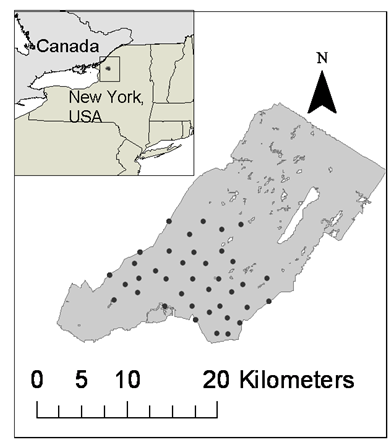
\includegraphics[height=2.5in,width=1.9in]{hairsnares.png}
\caption{Fort Drum study area and hair snare locations.}
\label{fig.3.bears1}
\end{figure}

\begin{verbatim}
# Consider adding comments to your code.   
## Good idea. This will be done in final draft
trapmat<-read.csv("FDtrapmat.csv")
bearArray<-source("FDbeararray.R")$value
nind<-dim(bearArray)[1]
K<-dim(bearArray)[3]
ntraps<-dim(bearArray)[2]

M=175
nz<-M-nind

Xaug <- array(0, dim=c(M,ntraps,K))
Xaug[1:nind,,]<-bearArray
y<- apply(Xaug,c(1,3),sum)
y[y>1]<-1
ytot<-apply(y,1,sum)   # total encounters out of K
\end{verbatim}

Note that the raw data, ${\bf y}$, is an $M \times K$ array of
individual encounter events (i.e., $y_{ik} = 1$ if individual $i$ was
encountered in any trap and 0 otherwise).  For $i=48,...,175$,
$y_{ik}$=0 as these are augmented observations.  For Model M0 it is
sufficient to reduce the data to individual encounter frequencies
which we have labeled \mbox{\tt ytot} above.  The BUGS model file
along with commands to fit the model are as follows:

\begin{verbatim}
cat("
model {

psi~dunif(0, 1)
p~dunif(0,1)

for (i in 1:M){
   z[i]~dbern(psi)
   for(k in 1:K){
      tmp[i,k]<-p*z[i]
      y[i,k]~dbin(tmp[i,k],1)
       }
       }
N<-sum(z[1:M])
}
",file="modelM0.txt")

data0<-list(y=y,M=M,K=K)
params0<-list('psi','p','N')
zst=as.vector(rbinom(M, 1, .5))
inits =  function() {list(z=zst, psi=runif(1), p=runif(1)) }
fit0 = bugs(data0, inits, params0, model.file="modelM0.txt",working.directory=getwd(),    
       debug=TRUE, n.chains=3, n.iter=2000, n.burnin=1000, n.thin=1)
\end{verbatim}

The posterior distributions of the model parameters are shown in
Fig. XYZ (maybe not) and summary statistics are provided in the
following table. In particular the posterior mean of $N$ under this
model is $49.99$ and a 95\% posterior interval is $(47,55)$.  We
revisit these data later in the context of more complex models.

\begin{verbatim}
Node statistics
node	 mean	 sd	 MC error    2.5%	median	97.5%	
N	49.99	1.961	0.05465	     47.0	50.0	55.0	
p 	 0.3016	0.02474	6.036E-4      0.2533	 0.3017	 0.3496	
psi	 0.288	0.03519	7.989E-4      0.221	 0.2868	 0.3621	
dic.stats()
\end{verbatim}

In order to obtain an estimate of density, $D$, we need an area to
associate with the estimate of $N$, and commonly used procedures to
conjure up such an area include buffering the trap array by the home
range radius, often estimated by the mean maximum distance moved
(MMDM)\footnote{really MMDM? How can this be an estimate of the home
  range radius?} or $1/2$ MMDM \citep{dice:1938}. Typically, the trap
array is defined by the convex hull around the trap locations, and
this is what we applied a buffer to. We computed the buffer by using
an estimate of the mean female home range radius estimated from
telemetry studies \citep{bales_etal:2005} instead of using an estimate
based on our relatively more sparse recapture data\footnote{Why? Just
  b/c less data?}. For the Fort Drum study, the convex hull has area
$157.135$ $km^2$, and the buffered convex hull has area $255.3$
$km^2$.  ({\bf These numbers are all wrong -- need to change buffer
  size}) Because the state-space area is {\it fixed} and known, the
density estimate under model $M_0$ can be obtained by summarizing the
appropriate function of the model parameter $N$ as follows:

{\bf Wrong buffer below}

\begin{verbatim}
> summary(fit0$sims.list$N/255.3)
   Min. 1st Qu.  Median    Mean 3rd Qu.    Max. 
 0.1841  0.1919  0.1958  0.1963  0.1998  0.2389 
\end{verbatim}
which yields a density estimate of $0.195$ ind/km$^2$, and a $95\%$ Bayesian 
confidence interval of:
\begin{verbatim}
> quantile(fit0$sims.list$N/255.3,c(0.025,0.975))
     2.5%     97.5% 
0.1840971 0.2154328 
\end{verbatim}

The obvious limitation of this estimate and, indeed, of the whole
process, is that our choice of ``area'' is completely subjective -
which area should we use? MMDM? One-half MMDM? Estimated from
telemetry data? And, furthermore, how certain are we of this area?
i.e., what is its ``standard error''?  More important, what exactly is
the meaning of this area and in this context how do we gauge bias
and/or variance of ``estimators'' of it? (i.e., what is it
estimating?).


\section{Temporally varying and behavioral effects}

The purpose of this chapter is mainly to emphasize the central
importance of the binomial model in capture-recapture and so we have
considered models for individual encounter frequencies - the number of
times individuals are captured out of $K$ samples.  Sometimes it is
not acceptable to aggregate the encounter data for each individual -
such as when encounter probability varies over time among samples. A
type of time-varying response that seems relevant in most
capture-recapture studies is ``effort'' such as amount of search time,
number of observers, or trap effort.  A common situation is that in
which there exists a ``behavioral response'' to trapping (even if the
animal is not physically trapped) or perhaps when $p$ depends on date
\citep{kery_etal:2010, gardner_etal:2010}.

Behavioral response is an important concept in carnivore studies
because individuals might learn to come to baited traps or avoid traps
due to trauma related to being encountered.  There are a number of
ways to parameterize a behavioral response to encounter. The
distinction between persistent and ephemeral was made by
\citet{yang_chao:2005} who considered a general behavioral response
model of the form:
\[
\mbox{logit}(p_{ik}) = \alpha_{0} + \alpha_{1}*y_{i,k-1} + \alpha_{2} x_{ik}
\]
where $x_{ik}$ is a covariate indicator variable of previous capture
(i.e., $x_{ik} = 1$ if captured in any previous period). Therefore,
encounter probability changes depending on whether an individual was
captured in the immediate previous period (ephemeral behavioral
response) or in any previous period (persistent behavioral
response). The former probably models a behavioral response due to
individuals moving around their territory relatively slowly over time
and the latter probably accommodates trap happiness due to baiting or
shyness due to trauma.  In spatial capture-recapture models it makes
sense to consider a local behavioral response that is trap-specific
\citep{royle_etal:2011} - that is, the encounter probability is
modified for individual traps depending on previous capture in
specific traps.

Models with temporal effects are easy to describe in the BUGS language 
and analyze and we provide a number of examples in chapt. 8.


\section{ Models with individual heterogeneity}

Here we consider models with individual-specific encounter probability
parameters, say $p_{i}$, which we model according to some probability
distribution, $g(\theta)$. We denote this basic model assumption as
$p_{i} \sim g(\theta)$. This type of model is similar in concept to
extending a GLM to a GLMM but in the capture-recapture context $N$ is
unknown.  The basic class of models is often referred to as ``Model
Mh'' but really this is a broad class of models, each being
distinguished by the specific distribution assumed for $p_{i}$.  There
are many different varieties of Model $M_{h}$ including parametric and
various putatively non-parametric approaches
\citep{burnham_overton:1978, norris_pollock:1996, pledger:2000}. One
important practical matter is that estimates of $N$ can be extremely
sensitive to the choice of heterogeneity model
\citep{fienberg_etal:1999, dorazio_royle:2003, link:2003}. Indeed,
\citet{link:2003} showed that in some cases it's possible to find
models that yield precisely the same expected data, yet produce wildly
different estimates of $N$. In that sense, $N$ for most practical
purposes is not identifiable across classes of mixture models, and
this should be understood before fitting any such model. One solution
to this problem is to seek to model explicit factors that contribute
to heterogeneity, e.g., using individual covariate models (See
\ref{closed.sec.indcov} below). Indeed, spatial capture-recapture
models seek to do just that, by modeling heterogeneity due to the
spatial organization of individuals in relation to traps or other
encounter mechanism.  For additional background and applications of
Model $M_{h}$ see \citet[][chapt. 6]{royle_dorazio:2008} and
\citet[][chapt. xxx]{kery_schaub:2011}.


Model $M_{h}$ has important historical relevance to spatial
capture-recapture situations \citep{karanth:1995} because
investigators recognized that the juxtaposition of individuals with
the array of trap locations should yield heterogeneity in encounter
probability, and thus it became common to use some version of Model Mh
in spatial trapping arrays to estimate $N$.  While this doesn't
resolve the problem of not knowing the area relevant to $N$, it does
yield an estimator that accommodates the heterogeneity in $p$ induced
by the spatial aspect of capture-recapture studies.

To see how this juxtaposition induces heterogeneity, we have to
understand the relevance of movement in capture-recapture models.
Imagine a quadrat that can be uniformly searched by a crew of
technicians for some species of reptile (see
\citet{royle_young:2008}).  Figure \ref{fig.3.quadrat} below shows a
sample quadrat searched repeatedly over a period of time. Further,
suppose that species exhibits some sense of spatial fidelity in the
form of a home range or territory, and individuals move about their
home range (home range centroids are given by the blue dots) in some
kind of random fashion.  It is natural to think about it in terms of a
movement process and sometimes that movement process can be modeled
explicitly using hierarchical models \citep{royle_young:2008,
  royle_etal:2011}.  Heuristically, we imagine that each individual in
the vicinity of the study area is liable to experience variable
exposure to encounter due to the overlap of its home range with the
sampled area - essentially the long-run proportion of times the
individual is within the sample plot boundaries, say $\phi_{i}$. We
might model the exposure of an individual to capture by supposing that
$z_{i} = 1$ if individual $i$ is available to be captured (i.e.,
within the survey plot) during any sample, and 0 otherwise. Then,
$\Pr(z_{i}=1) = \phi$.  In the context of spatial studies, it is
natural that $\phi$ should depend on {\it where} an individual lives,
i.e., it should be individual-specific $\phi_{i}$
\citep{chandler_etal:2011}. This system describes, precisely, that of
``random temporary emigration'' \citep{kendall_etal:1997} where $\phi$
is individual-specific.  Conceptually, SCR models aim to deal with
this problem of variable exposure to sampling due to movement in the
proximity of the trapping array explicitly and formally with auxiliary
spatial information.  If individuals are detected with probability
$p_{0}$, {\it conditional} on $z_{i} = 1$, then the marginal
probability of detection of individual $i$ is
\[
 p_{i} = p_{0}\phi_{i}
\]
so we see clearly that individual heterogeneity in encounter
probability is induced as a result of the juxtaposition of individuals
(i.e., their home ranges) with the sample apparatus and the movement
of individuals about their home range.

\begin{figure}
\begin{center}
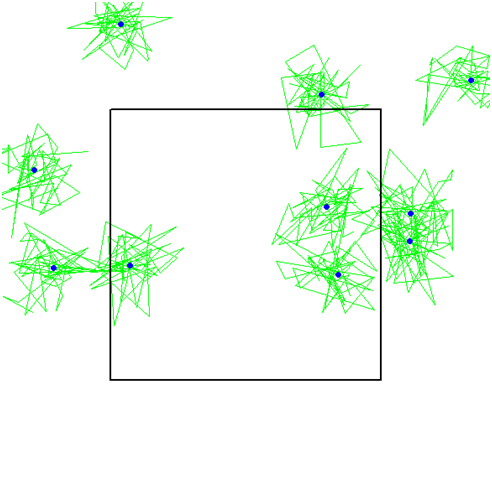
\includegraphics[height=3in]{quadrat}
\end{center}
\caption{Needs a caption}
\label{fig.3.quadrat}
\end{figure}


We will work with a specific type of Model $M_{h}$ here, that in which
we extend the basic binomial observation model of Model $M_{0}$ so
that
\[
\mbox{logit}(p_{i}) = \mu + \eta_{i}  
\]
where 
\[
\eta_{i} \sim \mbox{Normal}(0, \sigma_{p}^2)
\]
We could as well write
\[
	\mbox{logit}(p_{i}) \sim \mbox{Normal}(\mu,\sigma_{p}^2)
\]
This ``logit-normal mixture'' was analyzed by
\citet{coull_agresti:1999} and elsewhere. It is a natural extension of
the basic model with constant $p$, as a mixed GLMM, and similar models
occur throughout statistics. It is also natural to consider a beta
prior distribution for $p_{i}$ \citep{dorazio_royle:2003} and
so-called ``finite-mixture'' models are also popular
\citep{norris_pollock:1996, pledger:2000}.



\subsection{Analysis of Model Mh}

If $N$ is known, it is worth taking note of the essential simplicity
of Model Mh as a binomial GLMM.  This is a type of model that is
widely applied in just about every scientific discipline and using
standard methods of inference based either on integrated likelihood
\citep{laird_ware:1982, berger_etal:1999} or standard Bayesian
methods. However, because $N$ is not known, inference is somewhat more
challenging. We address that here using Bayesian analysis based on
data augmentation. Although we use Bayesian methods here, we note that
heterogeneity models formulated under DA are easily analyzed by
conventional likelihood methods as zero-inflated binomial mixtures
\citep{royle:2006} and more traditional analysis of model Mh based on
integrated likelihood, without using data augmentation, has been
considered by \citet{coull_agresti:1999}, \citet{dorazio_royle:2003},
and others.

As with model $M_{0}$, we have the Bernoulli model for the
zero-inflation variables: $z_{i} \sim \mbox{Bern}(\psi)$ and the model
of the observations expressed conditional on the latent variables
$z_{i}$. For $z_{i}=1$, we have a binomial model with
individual-specific $p_{i}$:
\[
y_{i}|{z_{i} \! = \! 1} \sim \mbox{Bin}(K,p_{i})
\]
and otherwise $y_{i} |{ z_{i} \! = \! 0} \sim \delta(0)$. Further, we
prescribe a distribution for $p_{i}$. Here we assume
\[
\mathrm{logit}(p_{i}) \sim \mbox{Normal}(\mu,\sigma^2)
\]
The basic BUGS description for this model, assuming a
$\mbox{Unif}(0,1)$ prior for $p_{0} = \mbox{logit}^{-1}(\mu)$ is given
as follows:
\begin{verbatim}
model{

p0 ~ dunif(0,1)       # prior distributions
mup<- log(p0/(1-p0))
taup~dgamma(.1,.1)
psi~dunif(0,1)

for(i in 1:(nind+nz)){
  z[i]~dbern(psi)     # zero inflation variables
  lp[i] ~ dnorm(mup,taup) # individual effect
  logit(p[i])<-lp[i]
  mu[i]<-z[i]*p[i]
  y[i]~dbin(mu[i],J)  #  observation model
 }

N<-sum(z[1:(nind+nz)])
}
\end{verbatim}
 


\subsection{Analysis of Fort Drum data}

The logit-normal heterogeneity model was fitted to the bear data from
the Fort Drum study producing the posterior distribution for $N$ shown
in Figure \ref{fig.bearMh}. Posterior summaries of parameters are
given in Table \ref{tab.Mh}.  We used $M=350$ for this analysis and we
note that the posterior mass of $N$ is located well away from this
upper bound (Figure XYZ), indicating that sufficient data augmentation
was used.  To fit this model to the Fort Drum data, the reader can use
the BUGS model description above in conjunction with the script
provided for Model M0 in section XXXXX.  Additional R commands for
organizing the black bear data and setting things up for WinBUGS are
provided in the Online Supplement.

The posterior mode compares well with the MLE which we obtained using
the R code contained in Panel 6.1 of \citet{royle_dorazio:2008}.  The
MLE of $log(n_{0})$, the logarithm of the number of uncaptured
individuals, is $log(n0) = 3.86$ and therefore the MLE is $\hat{N} =
exp(3.86)+47 = 94.47$ consistent with the apparent mode in Figure XYZ.
\footnote{We note that the result is inconsistent with Gardner et
  al. (2009) who reported an MLE of 104.1 ($density = 0.437
  inds/km^2$) although we do not know the reason for this at the
  present time.}  To convert this to density we use the buffered area
as computed above (255.3 $km^2$)\footnote{WRONG \#} and perform the
required summary analysis on the posterior samples of $N$, which
results in about $0.37$ individuals/$km^2$. The reader should carry
out this analysis to confirm the estimates, and also obtain the $95\%$
confidence interval.

\begin{verbatim}
\begin{table}
\centering
\caption{
Parameter estimates for Model $M_{h}$ (logit-normal model for 
 $p$)   fitted  to the Fort Drum hair-snare study data.
 Get final estimates and then tabularize this.
}
\begin{tabular}{lrrrrr}
\hline
node	 mean	 sd	 MC error	2.5%	median	97.5%	start	sample
N	111.6	48.15	2.413	61.0	97.0	250.0	1001	30000
deviance	185.8	17.6	0.4929	154.8	184.6	223.0	1001	30000
p0	0.07999	0.05713	0.002736	0.004606	0.06944	0.208	1001	30000
psi	0.3201	0.1388	0.006863	0.1643	0.2808	0.7163	1001	30000
sigmap	1.992	0.5087	0.02465	1.17	1.935	3.135	1001	30000
\end{tabular}
\label{tab.Mh}
\end{table}
\end{verbatim}

\begin{verbatim}
\begin{figure}
\centering
\includegraphics[height=2.0in,width=4.0in]{tigerMh_Npost}
\caption{Posterior of $N$ for Fort Drum bear study data under the
logit-normal version of model $M_h$. We will reproduce this from R.
XXX The picture is not the correct picture.   }
\label{fig.bearMh}
\end{figure}
\end{verbatim}

\subsection{Building your own MCMC algorithm}

For fun, we construct our own MCMC algorithm using a Metropolized
Gibbs sampler.  In Chapter \ref{chapt.mcmc} we devise an MCMC
algorithm for a spatial capture-recapture model and the basic
conceptual and technical considerations are entirely analogous to
Model Mh.

To begin, we identify the joint posterior distribution which we know
is proportional to the joint distribution of all elements
$y_{i},p_{i},z_{i}$ and also the prior distributions of $\mu_{p}$ and
$\sigma_{p}$, and the data augmentation parameter $\psi$:
\[
\left\{ \prod_{i=1}^{M} [y_{i}|p_{i},z_{i}][p_{i}|\mu_{p},\sigma_{p}]
[z_{i}|\psi] \right\} [\mu_{p},\sigma_{p},\psi]
\]
For prior distributions, we assume that $\mu_{p},\sigma_{p}, \psi$ are
mutually independent and for $\mu_{p}$ and $\sigma_{p}$ we use
improper uniform priors, and $\psi \sim \mbox{Unif}(0,1)$.  Note that
the likelihood contribution for each individual, when conditioned on
$p_{i}$ and $z_{i}$, does not depend on $\psi$, $\mu_{p}$, or
$\sigma_{p}$.  As such, the full-conditionals for the structural
parameters $\psi$ only depends on the collection of data augmentation
variables $z_{i}$, and that for $\mu_{p}$ and $\sigma_{p}$ will only
depend on $p_{i}$.  The full conditionals for all the unknowns are:

\begin{itemize}
\item (1) $[p_{i}|y_{i}, \mu_p, \sigma_{p},z_{i}=1] \propto 
[y_{i}|p_{i}][p_{i}|\mu_p,\sigma_{p}^{2}]$ if $z_{i}=1$ 
 $[p_{i}|\mu_p,\sigma_{p}]$ if $z_{i}=0$
\item (2)  $z_{i} | \cdot \propto [y_{i}|z_{i}*p_{i}]*\mbox{Bern}(z_{i}|\psi)$
\item (3) $\mu_{p} \sim \prod_{i} [p_{i}| \cdot] *\mbox{const}$
\item (4) $\sigma_{p}|\cdot \sim\prod_{i}[p_{i}| \cdot ]*\mbox{const}$
\item (5) $\psi|\cdot\sim \mbox{Beta}(\cdot, \cdot)$
\end{itemize}

What we've done here is identify each of the full conditional
distributions in sufficient detail to toss them into our
Metropolis-Hastings algorithm. With the exception of $\psi$ which has
a convenient analytic solution - it is a beta distribution which we
can easily sample directly. In truth, we could also sample $\mu_{p}$
and $\sigma_{p}^{2}$ directly with certain choices of prior
distributions. For example, if $\mu_{p} \sim \mbox{Normal}(0, 1000)$
then the full conditional for $\mu_{p}$ is also normal.

We implement an MCMC algorithm for this model in the following block
of {\bf R} code.  The basic structure is: initialize the parameters
and create any required output or intermediate ``holders'', and then
begin the main MCMC loop which, in this case, generates 100000
samples.

\begin{verbatim}

## obtain the bear data by executing the previous data grabbing
## function 

temp<-getdata()
M<-temp$M 
K<-temp$K
ytot<-temp$ytot


### 
### MCMC algorithm for Model Mh

out<-matrix(NA,nrow=100000,ncol=4)
dimnames(out)<-list(NULL,c("mu","sigma","psi","N"))
lp<- rnorm(M,-1,1)
p<-expit(lp)
mu<- -1
p0<-exp(mu)/(1+exp(mu))
sigma<- 1
psi<- .5 
z<-rbinom(M,1,psi)
z[ytot>0]<-1

for(i in 1:100000){

### update the logit(p) parameters
lpc<- rnorm(M,lp,1)  # 0.5 is a tuning parameter
pc<-expit(lpc)
lik.curr<-log(dbinom(ytot,K,z*p)*dnorm(lp,mu,sigma))
lik.cand<-log(dbinom(ytot,K,z*pc)*dnorm(lpc,mu,sigma))
kp<- runif(M) < exp(lik.cand-lik.curr)
p[kp]<-pc[kp]
lp[kp]<-lpc[kp]

p0c<- rnorm(1,p0,.05)
if(p0c>0 & p0c<1){
muc<-log(p0c/(1-p0c))
lik.curr<-sum(dnorm(lp,mu,sigma,log=TRUE))
lik.cand<-sum(dnorm(lp,muc,sigma,log=TRUE))
if(runif(1)<exp(lik.cand-lik.curr)) {
 mu<-muc
 p0<-p0c
}
}

sigmac<-rnorm(1,sigma,.5)
if(sigmac>0){
lik.curr<-sum(dnorm(lp,mu,sigma,log=TRUE))
lik.cand<-sum(dnorm(lp,mu,sigmac,log=TRUE))
if(runif(1)<exp(lik.cand-lik.curr)) 
 sigma<-sigmac
}

### update the z[i] variables
zc<-  ifelse(z==1,0,1)  # candidate is 0 if current = 1, etc..
lik.curr<- dbinom(ytot,K,z*p)*dbinom(z,1,psi)
lik.cand<- dbinom(ytot,K,zc*p)*dbinom(zc,1,psi)
kp<- runif(M) <  (lik.cand/lik.curr)
z[kp]<- zc[kp]

psi<-rbeta(1, sum(z) + 1, M-sum(z) + 1) 

out[i,]<- c(mu,sigma,psi,sum(z))
}
\end{verbatim}

{\bf Remarks}: (1) for parameters with bounded support, i.e.,
$\sigma_{p}$ and $p_{0}$, we are using a random walk candidate
generator but rejecting draws outside of the parameter space.  (2) We
mostly use Metropolis-Hastings except for the data augmentation
parameter $\psi$ which we sample directly from its full-conditional
distribution which is a beta distribution.  (3) Even the latent data
augmentation variables $z_{i}$ are updated using Metropolis-Hastings
although they too can be updated directly from their full-conditional.

\subsection{Exercises related to model Mh}

\begin{itemize}
\item[(1)] Enclose the MCMC algorithm in an R function and provide
  arguments for some of the parameters of the function that a user
  might wish to modify.
\item[(2)] Execute the function and compare the results to those
  generated from WinBUGS in the previous section
\item[(3)] Note that the prior distribution for the ``mean'' parameter
  is given on $p_0=exp(\mu)/(1+exp(\mu))$.  Reformulate the algorithm
  with a flat prior on $\mu$ and see what happens. Contemplate this.
\item[(4)] Using Bayes rule, figure out the full conditional for
  $z_{i}$ so that you don't have to use MH for that one. It might be
  more efficient. Is it?
\end{itemize}


\section{Individual Covariate Models: Toward Spatial Capture-Recapture}
\label{closed.sec.indcov}

A standard situation in capture-recapture models is when an individual
covariate is measured, and this covariate is thought to influence
encounter probability.  As with other closed population models, we
begin with the basic binomial observation model:
\[
y_{i} \sim \mbox{Bin}(K, p_{i})
\]
and we assume also  a model for encounter probability according to:
\[
 \mbox{logit}(p_{i}) = \alpha_{0} + \alpha_{1} x_{i}
\]
Classical examples of covariates influencing detection probability are
type of animal (juvenile/adult or male/female), a continuous covariate
such as body mass \citep[][chapt. 6]{royle_dorazio:2008}, or a
discrete covariate such as group or cluster size. For example, in
models of aerial survey data, it is natural to model detection
probabilities as a function of the observation-level individual
covariate, ``group size'' \citep{royle:2008, royle:2009,
  langtimm_etal:2010}.

Such ``individual covariate models'' are similar in structure to Model
$M_{h}$, except that the individual effects are {\it observed} for the
$n$ individuals that appear in the sample. These models are important
here because spatial capture-recapture models are precisely a form of
individual covariate model, an idea that we will develop here and
elsewhere. Specifically, they are such models, but where the
individual covariate is a partially observed latent variable similar..
That is, unlike Model Mh, we do have some direct information about the
latent variable, which comes from the spatial locations/distribution
of individual recaptures. More on that later.

Traditionally, estimation of $N$ in individual covariate models is
achieved using methods based on ideas of unequal probability sampling
(i.e., Horwitz-Thompson estimation), see \citet{huggins:1989} and
\citet{alho:1990}. An estimator of $N$ is
\[
\hat{N} = \sum_{i} \frac{1}{\tilde{p}_{i}}
\]
where $\tilde{p}_{i}$ is the probability that individual $i$ appeared
in the sample.  That is, $\tilde{p}_{i} = \Pr(y_{i}>0)$.  In practice,
$\tilde{p}_{i}$ is estimated from the conditional-likelihood formed by
the encounter histories. Namely,
\[
\Pr(y_{i}|y_{i}>0) = \Pr(y_{i})/\Pr(y_{i}>0)
\]
where we substitute
\[
\Pr(y_{i}>0) = (1- (1-p_{i})^K) 
\]
with 
\[
\mbox{logit}(p_{i}) = \alpha_{0} + \alpha_{1} x_{i}
\]

Here we take a formal model-based approach to Bayesian analysis of
such models using data augmentation \citep{royle:2009}. Classical
likelihood analysis of the so-called ``full likelihood'' is covered in
some detail by \citet{borchers_etal:2002}.  For Bayesian analysis of
individual covariate models, because the individual covariate is
unobserved for the $N-n$ uncaptured individuals, we require a model to
describe variation among individuals, essentially allowing the sample
to be extrapolated to the population.  For our present purposes, we
consider a continuous covariate and we assume that it has a normal
distribution:
\[
x_{i} \sim \mbox{Normal}(\mu,\sigma^{2})
\]

Data augmentation can be applied directly to this class of models. In
particular, reformulation of the model under DA yields a basic
zero-inflated binomial model of the form:
\begin{eqnarray*}
z_{i} &\sim& \mbox{Bern}(\psi) \\
y_{i}|{z_{i}\! =\! 1} &\sim& \mbox{Bin}(K,p_{i}) \\
y_{i} |{ z_{i}\! =\! 0} &\sim& \delta(0)  \\
\end{eqnarray*}
In addition, we assume that $p_{i}$ is functionally related to a
covariate $x_{i}$, e.g., by the logit model given above, and we assume
a distribution for $x_i$ appropriate for the context.

Fully spatial capture-recapture models essentially use this
formulation with a latent covariate that is directly related to the
individual detection probability (see next Section). As with the
previous models, implementation is trivial in the BUGS language. The
BUGS specification is very similar to that for model $M_h$, but we
require the distribution of the covariate to be specified, along with
priors for the parameters of that distribution.


\subsection{Example: Location of capture as a covariate.}

If we had a regular grid of traps over some closed geographic system
then we imagine that the average location of capture would be a decent
estimate (heuristically) of an individual's home range center.
Intuitively some measure of typical distance from home range center to
traps for an individual should be a decent covariate to explain
heterogeneity in encounter probability, i.e., individuals with more
exposure to traps should have higher encounter probabilities and vice
versa.  A version of this idea was put forth by
\citet{boulanger_mclellan:2001} (see also \citet{ivan:2012}), but
using the Huggins-Alho estimator and with covariate ``distance to
edge'' of the trapping array. A limitation of this basic approach is
that it does not provide a solution to the problem that the trap area
is fundamentally ill-defined, nor does it readily accommodate the
inherent and heterogeneous variation in this measured covariate.
Here, we provide an example of this type of heuristically motivated
approach using the fully model-based individual covariate model
described above analyzed by data augmentation. We take a slightly
different approach than that adopted by
\citet{boulanger_mclellan:2001}. By analyzing the full likelihood and
placing a prior distribution on the individual covariate, we resolve
the problem of having an ill-defined area over which the population
size is distributed. After you read later chapters of this book, it
will be apparent that SCR models represent a formalization of this
heuristic procedure.

For our purposes here, we define $x_{i} = ||s_{i} - x_{0}||$ where $s_{i}$
is the average encounter location of individual $i$ and $x_{0}$ is the
centroid of the trap array.  Conceptually, individuals in the middle
of the array should have higher probability of encounter and, as
$x_{i}$ increases, $p_{i}$ should therefore decrease. We note that we
have defined $s_{i}$ in terms of a sample quantity - the observed mean
- which is ad hoc but maybe satisfactory under the circumstances. That
said, for
an expansive, dense trapping grid then we might expect the sample mean
encounter location to be a good estimate of home range center but,
clearly this is biased for individuals that live around the edge (or
off) the trapping array. Regardless, it should be good enough for our
present purposes of demonstrating this heuristically appealing
application of an individual covariate model. A key point is that
$s_{i}$ is missing for each individual that is not encountered and
thus so is $x_{i}$. Thus,
it is a latent variable, or random effect, and we need therefore to
specify a probability distribution for it.  
As a measurement of distance we know it must be
positive-valued. Suppose further than we imagine no individual could
have a home range radius larger than $D_{max}$. As such, we think a
reasonable distribution for this individual covariate is
\[
 x_{i} \sim uniform(0,D_{max})
\]
where $D_{max}$ is a specified constant.  In practice, people have
used distance from edge of the trap array but that is less easy to
define and compute.


\subsubsection{Fort Drum Bear Study} 

We have to do a little bit of data processing to fit this individual
covariate model to the Fort Drum data. To compute the average location
of capture for each individual and the distance from the centroid of
the trap array, we execute the following R instructions:

\begin{verbatim}
avg.s<-matrix(NA,nrow=nind,ncol=2)
for(i in 1:nind){
tmp<-NULL
for(j in 1:T){
aa<-bearArray[i,,j]
if(sum(aa)>0){
 	aa<-  trapmat[aa>0,]
 	tmp<-rbind(tmp,aa)
}
}
avg.s[i,]<-c(mean(tmp[,1]),mean(tmp[,2]))
}
Cx<-mean(trapmat[,1])
Cy<-mean(trapmat[,2])
avg.s<-rbind(avg.s,matrix(NA,nrow=nz,ncol=2))
xcent<- sqrt( (avg.s[,1]-Cx)^2 +  (avg.s[,2]-Cy)^2)
\end{verbatim}

To define the maximum distance (maxD) from the centroid, we use that
of the farthest trap, and so maxD is computed as follows:

\begin{verbatim}
minx<- min(trapmat[,1]-Cx)
maxx<-max(trapmat[,1]-Cx)
miny<- min(trapmat[,2]-Cy)
maxy<- max(trapmat[,2]-Cy)
# most extreme point determines maxD
ul<- c(minx,maxy)
maxD<- sqrt(  (ul[1]-0)^2 + (ul[2]-0)^2)
\end{verbatim}

For the bear data the maxD was about 11.5 km. As such, the model
described above will produce an estimate of the population size of
bears within 11.5 units of the trap centroid\footnote{To be convincing
  this might  need a little bit of hand-holding}. The BUGS model
specification and R commands to package the data and fit the model are
as follows:

\begin{verbatim}
cat("
model{
p0 ~ dunif(0,1)       # prior distributions
mup<- log(p0/(1-p0))
psi~dunif(0,1)
beta~dnorm(0,.01)

for(i in 1:(nind+nz)){
  xcent[i]~dunif(0,maxD)
  z[i]~dbern(psi)     # DA variables
  lp[i] <- mup + beta*xcent[i] # individual effect
  logit(p[i])<-lp[i]
  mu[i]<-z[i]*p[i]
  y[i]~dbin(mu[i],K)  #  observation model
 }
N<-sum(z[1:(nind+nz)])
}
",file="modelMcov.txt")
data2<-list(y=ytot,nz=nz,nind=nind,K=T,xcent=xcent,maxD=11.5)
params2<-list('p0','psi','N','beta')
inits =  function() {list(z=z, psi=psi, p0=runif(1),beta=rnorm(1) ) }
fit2 = bugs(data2, inits, params2, model.file="modelMcov.txt",working.directory=getwd(),    
       debug=T, n.chains=3, n.iter=4000, n.burnin=1000, n.thin=4)
\end{verbatim}

Posterior summaries are given in Table \ref{tab.maxD} XYZ, and the posterior distribution of $N$ is given in Figure XYZ. It might be perplexing that the estimated N is much lower than obtained by model Mh but there is a good explanation for this, discussed subsequently. That issue notwithstanding, it is worth pondering how this model could be an improvement (conceptually or technically) over some other model/estimator including M0 and Mh considered previously. Well, for one, we have accounted formally for heterogeneity due to spatial location of individuals relative to exposure to the trap array, characterized by the centroid of the array. Moreover, we have done so using a model that is based on an explicit mechanism, as opposed to a phenomenological one such as Model Mh. Moreover, importantly, using our new model, {\it the estimated N applies to an explicit area which is defined by our prescribed value of maxD}. That is, this area is a fixed component of the model and the parameter N therefore has explicit spatial context, as the number of individuals with home range centers less than maxD from the centroid of the trap array. As such, the implied ``effective trap area''\footnote{This is a bad use of this term. We have never defined ETA or ESA. What is it, exactly?} for any maxD is that of a circle with radius maxD. 

\begin{verbatim}
%% Not sure whether this should be a table or verbatim print-out
\begin{table}
\tabular{ccccccccc}
Node statistics
node	 mean	 sd	 MC error	2.5%	median	97.5%	start	sample
N	58.89	5.483	0.2199	50.0	58.0	71.0	251	2250
beta	-0.246	0.06087	0.003892	-0.3592	-0.2457	-0.126	251	2250
deviance	459.4	13.29	0.4496	435.7	458.4	487.8	251	2250
p0	0.5409	0.06817	0.004052	0.4072	0.544	0.6678	251	2250
psi	0.1706	0.02572	7.759E-4	0.1247	0.1692	0.2242	251	2250
\end{tabular}
\caption{..... xyz ......}
\end{table}
\label{tab.maxD}
\end{verbatim}

We'll remake this figure in R.  For now, insert it as is.

\begin{figure}
\begin{center}
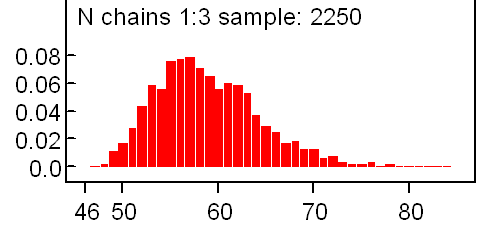
\includegraphics[width=3.5in]{Nchains}
\end{center}
\caption{Needs a caption}
\label{fig.nchains}
\end{figure}

\subsection{Extension of the Model}
One important issue in understanding the meaning of estimates produced under the individual covariate model  is that the uniform distribution on maxD implies that density is {\it not constant} over space. In particular, this model implies that it {\it decreases} as we move away from the centroid of the trap array. This is one reason we have a lower estimate of density than that obtained previously and also why, if we were to increase maxD, we would see density continue to decrease: $x[i] \sim \mbox{Uniform}(0,maxD)$ implies constant N in each distance band from the centroid but obviously the {\it area} of each distance band is increasing.  The reader can verify this as a homework exercise. 
Obviously, the use of an individual covariate model is {\it not} restricted to use of this specific distribution for the individual covariate. Clearly, it is a bad choice and, therefore,  we should think about whether we can choose a better distribution for maxD - one that doesn't imply a decreasing density as distance from the centroid increases.  Conceptually, what we want to do is impose a prior on distance from the centroid, $x$, such that density is proportional to the amount of area in each successive distance band as you move farther away from the centroid.  In fact, there is theory that exists which tells us what the correct distribution of $x$ is $2x/maxD^2$. This can be derived by noting that $F(x) = Pr(X<x) = pi*x*x/pi*maxD*maxD$ . Then, $f(x) = dF/dx = 2*x/(maxD*maxD)$.  This might be called a triangular distribution, I think, which makes sense because the incremental area in each additional distance band increases linearly with radius (i.e., distance from centroid). It is sometimes comforting to verify things empirically:
\begin{verbatim}
> u<-runif(10000,-1,1)
> v<-runif(10000,-1,1)
> d<- sqrt(u*u+v*v)
> hist(d[d<1])
> hist(d[d<1],100)
> hist(d[d<1],100,probability=TRUE)
> abline(0,2)
\end{verbatim}

It would be useful if we could describe this distribution in *BUGS but there is not a built-in way to do this.  One possibility is to use a discrete version of the pdf. We might also be able to use what is referred to in WinBUGS jargon as the ``zeros trick'' (see Advanced BUGS tricks) although we haven't pursued this approach. Instead, we consider using a discrete version and break Dmax into L distance classes of width $\delta$, with probabilities proportional to $2*x$. In particular, if the cut-points are $xg[1]=0,xg[2], \ldots, xg[L+1]=Dmax$ and the interval midpoints are $xm[i] = xg[i+1]-\delta$. Then, the interval probabilities are $p[i] = 2*xm[i]*delta/(Dmax*Dmax)$, which we can compute once and then send them to WinBUGS as data.

The R script is as follows. In the model description the variable $x$ (observed home range center) has been rounded so that the discrete version of the $f(x)$ can be used as described previously. The new variable labeled \mbox{\tt xround} is actually then the integer category label in units of delta from 0. Thus, to convert back to distance in the expression for $lp[i]$, \mbox{\tt xround[i]} has to be multiplied by $\delta$.

\begin{verbatim}
delta<-.2
xround<-xcent%/%delta  + 1
Dgrid<- seq(delta,maxD,delta)
xprobs<- delta*(2*Dgrid/(maxD*maxD))
xprobs<-xprobs/sum(xprobs)

cat("
model{
p0 ~ dunif(0,1)       # prior distributions
mup<- log(p0/(1-p0))
psi~dunif(0,1)
beta~dnorm(0,.01)

for(i in 1:(nind+nz)){
  xround[i]~dcat(xprobs[])
  z[i]~dbern(psi)                     # zero inflation variables
  lp[i] <- mup + beta*xround[i]*delta # individual effect
  logit(p[i])<-lp[i]
  mu[i]<-z[i]*p[i]
  y[i]~dbin(mu[i],K)  #  observation model
 }

N<-sum(z[1:(nind+nz)])
}
",file="modelMcov.txt")
\end{verbatim}

To fit the model we do this - keeping in mind that the data objects required below have been defined in previous analyses of this chapter:

\begin{verbatim}
data2<-list(y=ytot,nz=nz,nind=nind,K=T,xround=xround,xprobs=xprobs,delta=delta)
params2<-list('p0','psi','N','beta')
inits =  function() {list(z=z, psi=psi, p0=runif(1),beta=rnorm(1) ) }
fit = bugs(data2, inits, params2, model.file="modelMcov.txt",working.directory=getwd(),    
       debug=FALSE, n.chains=3, n.iter=11000, n.burnin=1000, n.thin=2)
\end{verbatim}

This is a useful model because it induces a clear definition of area in which the population of $N$ individuals reside. Under this model, that area is defined  by specification of maxD. We can apply the model for different values of maxD and observe that the estimated $N$ varies with $maxD$. Fortunately, we see empirically, that while N seems highly sensitive to the prescribed value of $maxD$, density seems to be invariant to $maxD$ as long as it is chosen to be sufficiently large. We fit the model for $maxD=12$ (points in close proximity to the trap arra)  to 20 for and the results are given in Table \ref{tab.xyz}.

\begin{table}
\caption{Table: Analysis of Fort Drum bear hair snare data using the individual covariate model, for different values of Dmax, the upper limit of the uniform distribution of `distance from centroid of the trap array' }
\begin{tabular}{cccc}
     maxD   mn    SD         
[1,]  12 0.230 0.038
[2,]  15 0.244 0.041
[3,]  17 0.249 0.044
[4,]  18 0.249 0.043
[5,]  19 0.250 0.043
[6,]  20 0.250 0.044
\end{tabular}
\end{table}
%ANDY - I couldn't get this to show up right, I'll look into it if I
%get a chance


We see that the posterior mean and SD of density (individuals per square km) appear insensitive to choice of $maxD$ once we get a slight ways away from the maximum observed value of about 11.5. The estimated density of 0.250 per km$^2$ is actually quite a bit lower than we reported using model Mh (0.37, see section XYZ above) for which sample area is not an explicit feature of the model. On the other hand it is higher than that reported from Model M0 using the buffered area (0.195). There is no basis really for comparing or contrasting these various estimates and it would be a useful philosophical exercise for the reader to discuss this matter. In particular, application of model M0 and Mh are distinctly {\it not} spatially explicit models -- the area within which the population\footnote{We need to look back at Chapter 1 and make sure we quit calling this ``sample area'' - it really isn't that at al, but rather the area within which N resides.} resides is not defined under either model. There is therefore no reason at all to think that the estimates produced under either model, using a buffered area, are justifiable based on any theory. In fact, we would get exactly the same estimate of $N$ no matter what we declare the area to be. On the other hand, the individual covariate model explicitly describes a distribution for ``distance from centroid'' that is a reasonable and standard null model - it posits, in the absence of direct information, that individual home range centers are randomly distributed in space and that probability of detection depends on the distance between home range center and the centroid of the trap array. Under this definition of the system, we see that density is invariant to the choice of sample area which seems like a desirable feature. The individual covariate model is not ideal, however, because it does not make full use of the spatial information in the data set, i.e., the trap locations and the locations of each individual encounter. 


\subsection{Invariance of density to maxD} 

Under the model above, and also under models that we consider in later chapters, a general property of the estimators is that while N increases with the prescribed trap area (equivalent to maxD in this case), we expect that density estimators should be invariant to this area. In the model used above, we note that 
$Area(maxD) = \pi*maxD*maxD$ and $E[N(maxD)] = \lambda*A(maxD)$ and thus $E[Density(maxD)] = \lambda$  which is constant. This should be interpreted as the {\it prior} density. Absent data, then realizations under the model will have density $\lambda$ regardless of what $maxD$ is prescribed to be.  As we verified empirically above, the posterior density is also invariant if $maxD$ as long as the implied area (implied by maxD) is large enough so that the data no longer provide information about density (i.e., ``far away''), then our estimator of density should become insensitive. 

\subsection{Toward Fully Spatial Capture-recapture Models}
We developed this model for the average observed location and equated it to home range center $s_{i}$. Intuitively, taking the average encounter location as an estimate of home range center makes sense but more so when the trapping grid is dense and expansive relative to typical home range sizes.  However, our approach also ignored  the variable precision with which each $s[i]$ is estimated and also, as noted previously, estimates of $s[i]$ around the ``edge'' (however we define that) are biased because the observations are truncated (we can only observe locations within the trap array).  In the next Chapter we provide a further extension of this individual covariate model that definitively resolves the ad hoc nature of the individual covariate approach we took here. In that model we build a model in which $s[i]$ are regarded as latent variables and the observation locations (i.e., trap specific encounters) are linked to those latent variables with an explicit model. We note that the model fitted previously could be adapted easily to deal with $s_{i}$ as a latent variable, simply by adding a prior distribution for $s_{i}$. The reader should contemplate how to do this in WinBUGS. 


\section{DISTANCE SAMPLING: A primative Spatial Capture-Recapture Model} 

Distance sampling is one of the most popular methods for estimating
animal abundance. One of the great benefits of distance sampling is
that it provides explicit estimates of {\it density}. The distance
sampling model is a special case of a closed population model with a
covariate. The covariate in this case, $x_{i}$, is the distance
between an individual's location ``$u$'' and the observation location
or transect. In fact, the model underlying distance sampling is
precisely the same model as that which applies to the
individual-covariate models, except that observations are made at only
$K=1$ sampling occasion. In a sense, distance sampling is a spatial
capture-recapture model, but without the ``recapture.''  This first
and most basic spatial capture-recapture model has been used routinely
for decades and, formally, it is a spatially-explicit model in the
sense that it describes, explicitly, the spatial organization of
individual locations (although this is not always stated explicitly)
and, as a result, somewhat general models of how individuals are
distributed in space can be specified \citep{royle_etal:2004,
  johnson_etal:2010, sillett_etal:2011}. 
As before, the distance sampling model, under data augmentation, includes a set of $M$ zero-inflation variables $z_{i}$ and the binomial model expressed conditional on $z$ (binomial for $z=1$, and fixed zeros for $z=0$).  In distance sampling we pay for having only a single sample (i.e., $K=1$) by requiring constraints on the model of detection probability. A standard model is
\[
\log(p_{i}) = b * x_{i}^{2}
\]
for $b < 0$, where $x_i$ denotes the distance at which the $i$th
individual is detected relative to some reference location where
perfect detectability ($p=1$) is assumed. This function corresponds to
the ``half-normal'' detection function (i.e., with $b =
1/\sigma^{2}$).  If $K>1$ then the intercept alpha is identifiable and
such models are usually called ``capture-recapture distance
sampling''\citep{borchers_etal:XXXX} and others XYZ????).  

As with previous examples, we require a distribution for the individual covariate $x_{i}$. The customary choice is
\[
x_{i} \sim \mbox{Uniform}(0,B)
\]
wherein $B>0$ is a known constant, being the upper limit of data
recording by the observer (i.e., the point count radius, or transect
half-width). In practice, this is sometimes asserted to be infinity,
but in such cases the distance data are usually truncated.
Specification of this distance sampling model in the BUGS language is
shown in Panel \ref{panel.distance}. \citet{royle_dorazio:2008}, p. xyz) provide a distance sampling example analyzed by DA using the famous Impala data. 

\begin{panel}[htp]
\centering
\rule[0.15in]{\textwidth}{.03in}
\begin{minipage}{5in}
\begin{verbatim}
b~dunif(0,10)
psi~dunif(0,1)

for(i in 1:(nind+nz)){
   z[i]~dbern(psi)    # DA Variables
   x[i]~dunif(0,B)    # B=strip width
   p[i]<-exp(logp[i])   # DETECTION MODEL
   logp[i]<-   -((x[i]*x[i])*b)
   mu[i]<-z[i]*p[i]
   y[i]~dbern(mu[i])  # OBSERVATION MODEL
 }
N<-sum(z[1:(nind+nz)])
D<- N/striparea  # area of transects
\end{verbatim}
\end{minipage}
\rule[-0.15in]{\textwidth}{.03in}
\caption{Distance sampling model in WinBUGS, using a ``half-normal''
detection function.}
\label{panel.distance}
\end{panel}

As with the individual covariate model in the previous section, the distance sampling model can be equivalently specified by putting a prior distribution on individual {\it location} instead of distance between individual and observation point (or transect). 
Thus we can write the general distance sampling model as
\[
 logit(p[i]) = alpha + beta*||u[i] - x0||
\]
Along with
\[
 {\bf u}_{i} \sim Uniform({\cal S})
\]
where $x_{0}$ is a fixed point (or line) and $u[i]$ is the individual's location which is observable for n individuals. In practice it is easier to record distance instead of location.  Basic math can be used to argue that if individuals have a uniform distribution in space, then the distribution of Euclidean distance is also uniform. In particular, if a transect of length L is used and x is distance to the transect then $F(x) = Pr(X<=x) = L*x/L*B = x/B$ and $f(x) = dF/dx = (1/B)$. For measurements of radial distance, see the previous section. 

In the context of our general characterization of SCR models (chapter 1.XYZ), we suggested that every SCR model can be described, conceptually, by a hierarchical model of the form:
\[
 [y|u][u|s][s].
\]
Distance sampling ignores $s$, and treats u as observed data\footnote{Formally we could also say that $[u] = \int [y|s][s] ds$}. Thus, we are left with
\[
[y|u][u].
\]
In contrast, as we will see in the next chapters, basic SCR models (chapter 4) ignore $u$ and condition on $s$, which is not observed:
\[
[y|s][s]
\]
Since $[u]$ and $[s]$ are both assumed to be uniformly distributed, these are structurally equivalent  models! The main  differences have to do with interpretation of model components and whether or not the latent variables are observable (in distance sampling they are). 

So why bother with SCR models when distance sampling yields density estimates and accounts for spatial  heterogeneity in detection? For one, imagine try to collect distance sampling data on tigers! Clearly, distance sampling requires that one can collect large quantities of distance data, which is not always possible. For tigers, it is much easier, efficient, and safer to employ camera traps or tracking plates and then apply SCR models. Furthermore, as we will see in Ch XYZ, SCR models can use distance data to estimate all the parameters of our enchilada, allowing us to study distribution, movement, and density. Thus, SCR models are much more flexible than distance sampling models, and can accommodate data from virtually all animal survey designs. 


\subsection{Example: Muntjac deer survey from Nagarahole, India }
Here we fit distance sampling models to distance sampling data on the muntjac deer (Muntiakus muntjak) collected in the year 2004 from Nagarahole National Park in southern India \citep{kumar_etal:XXXX}(Kumar et al. unpublished data). The muntjac is a solitary species and distance measurements were made on 57 groups that were largely singletons with XYZ pairs of individuals.  Commands for reading in and organizing the data for WinBUGS, followed by writing the model to a text file. Note that the total sampled area of the transects is fed in as ``striparea'' which is 708 (km of transect) multiplied by the strip width (B=150 = 0.15 km) multiplied by 2.
\begin{verbatim}
library("R2WinBUGS")
data<- read.csv("Muntjac.csv")
nind<-nrow(data)
y<-rep(1,nind)
nz<-400
y<-c(y,rep(0,nz))
x<-data[,3]
x<-c(x,rep(NA,nz))
z<-y
data<-list(y=y,x=x,nz=nz,nind=nind,B=150,striparea=708*.15*2)

cat("
model{
b~dunif(0,10)
psi~dunif(0,1)

for(i in 1:(nind+nz)){
   z[i]~dbern(psi)    # DA Variables
   x[i]~dunif(0,B)    # B=strip width
   p[i]<-exp(logp[i])   # DETECTION MODEL
   logp[i]<-   -((x[i]*x[i])*b)
   #logp[i]<- -b*log(x[i]+1)
   mu[i]<-z[i]*p[i]
   y[i]~dbern(mu[i])  # OBSERVATION MODEL
 }
N<-sum(z[1:(nind+nz)])
D<- N/striparea  # area of transects
}
",file="dsamp.txt")
\end{verbatim}

Next, we provide inits, indicate which parameters to monitor, and then pass those things to WinBUGS:
\begin{verbatim}
params<-list('b','N','D','psi')
inits =  function() {list(z=z, psi=runif(1), b=runif(1,0,.02) )}
fit = bugs(data, inits,  params, model.file="dsamp.txt",
working.directory=getwd(),debug=T, n.chains=3, n.iter=4000, n.burnin=1000, n.thin=2)
\end{verbatim}
Posterior summaries are provided in the following table. Estimated density is pretty low, 1.1 individuals per sq. km.\footnote{ much lower than Samba's : Observers walked about 708 km from 39 transects in Nagarahole and the muntjac density is about 3 per sq km.. I need to get to the bottom of this.}
\begin{verbatim}
 node	 mean	 sd	 MC error	2.5%	median	97.5%	start	sample
D	1.096	0.1694	0.009122	0.8098	1.078	1.474	501	4500
N	232.8	35.99	1.938	172.0	229.0	313.0	501	4500
b	5.678E-4	1.05E-4	4.129E-6	3.867E-4	5.616E-4	7.949E-4	501	4500
deviance	681.2	16.72	0.7536	650.8	680.6	716.6	501	4500
psi	0.5099	0.08238	0.004442	0.3681	0.5033	0.6918	501	4500
\end{verbatim}


\section{Summary and Outlook}

Traditional closed population capture-recapture models are closely related to binomial generalized linear models.  Indeed, the only real distinction is that in capture-recapture models, the population size parameter $N$ (corresponding also to the size of a hypothetical ``complete'' data set) is unknown.  This requires special consideration in the analysis of capture-recapture models. The classical approach to inference recognizes that the observations don't have a standard binomial distribution but, rather, a truncated binomial (from which which the so-called ``conditional likelihood'' derives) since we only have encounter frequency data on observed individuals. If instead we analyze the models using data augmentation, the observations can be modeled using a zero-inflated binomial distribution. In short, when we deal with the unknown-N problem using data augmentation then we are left with zero-inflated GLM and GLMMs instead of ordinary GLM or GLMMs. The analysis of such zero-inflated models is practically convenient, especially using the various Bayesian analysis packages that use the BUGS language. 

Spatial capture-recapture models that we will consider in the rest of the chapters of this book are closely related to what have been called individual covariate models. Heuristically, spatial capture-recapture models arise by defining individual covariates based on observed locations of individuals -- we can think of using some function of mean encounter location as an individual covariate. We did this in a novel way, by using distance to the centroid of the trapping array as a covariate. We analyzed the ``full likelihood'' using data augmentation, and placed a prior distribution on the individual covariate which was derived from an assumption that individual locations are, a priori, uniformly distributed in space. This assumption provides for invariance of the density estimator to the choice of population size area (induced by maximum distance from the centroid of the). The model addressed some important problems in the use of closed population models: it allows for heterogeneity in encounter probability due to the spatial context of the problem and it also provides a direct estimate of density because area is a feature of the model (via the prior on the individual covariate). The model is still not completely general because the model does not make use of the fully spatial encounter histories, which provide direct information about the locations and density of individuals.
A specific individual covariate model that is in widespread use is
classical ``distance sampling.'' The model underlying distance sampling is precisely a special kind of SCR model - but one without replicate samples. Understanding distance sampling and individual covariate models more broadly provides a solid basis for understanding and analyzing spatial capture-recapture models. 


%\input{Chapter1.tex}
%\chapter{
Introduction to Bayesian Analysis of GL(M)Ms Using R/WinBUGS
}
\markboth{Chapter 2}{}
\label{chapt.intro}

\vspace{.3in}


A major theme of this book is that spatial capture-recapture models
are, for the most part, just generalized linear models (GLMs) wherein
the covariate, distance between trap and home range center, is
partially or fully unobserved  -- and therefore regarded as 
a random effect. Such models
are usually referred to as Generalized Linear Mixed Models (GLMMs)
and, therefore, SCR models can be thought of as a specialized type of
GLMM. Naturally then, we should consider analysis of these slightly
simpler models in order to gain some experience and, hopefully,
develop a better understanding of spatial capture-recapture models.

In this chapter, we consider classes of GLM models - Poisson and
binomial (i.e., logistic regression) GLMs - that will prove to be
enormously useful in the analysis of capture-recapture models of all
kinds. Many readers are probably familiar with these models because
they represent probably 
the most generally useful models in all of Ecology and, as
such, have received considerable attention in many introductory and
advanced texts. We focus on them here in order to introduce the
readers to the analysis of such models in {\bf R} and {\bf WinBUGS}, 
which we will
translate directly to the analysis of SCR models in subsequent
chapters.  

Bayesian analysis is convenient for analyzing GLMMs because it allows
us to work directly with the conditional model -- i.e., the model that
is conditional on the random effects, using computational methods
known as Markov chain Monte Carlo (MCMC). Learning how to do Bayesian
analysis of GLMs and GLMMs in {\bf WinBUGS} is, in part, the purpose
of this chapter.  While we use {\bf WinBUGS} to do the Bayesian
computations, we organize and summarize our data and execute {\bf
  WinBUGS} from within {\bf R} using the useful package \mbox{\tt
  R2WinBUGS} \citep{sturtz_etal:2005}.  \citet{kery:2010}, and
\citet{kery_schaub:2011} provide excellent introductions to the basics
of Bayesian analysis and GLMs at an accessible level. We don't want to
be too redundant with those books and so we avoid a detailed
treatement of Bayesian methodology - instead just providing a cursory
overview so that we can move on and attack the problems we're most
interested in related to spatial capture-recapture.  In addition,
there are a number of texts that provide general introductions to
Bayesian analysis, MCMC, and their applications in Ecology including
\citet{mccarthy:2007}, \citet{kery:2010}, \citet{link_barker:2009},and
\citet{king_etal:2009}.


While this chapter is about Bayesian analysis of GLMMs, such models
are routinely analyzed using likelihood methods too, as discussed by
\citet{royle_dorazio:2008}, and \citet{kery:2010}. Indeed, likelihood
analysis of such models is the primary focus of many applied
statistics texts, a good one being \citet{zuur_etal:2009}. Later in
this book, we will use likelihood methods to analyze SCR models but,
for now, we concentrate on providing a basic introduction to Bayesian
analysis because that is the approach we will use in a majority of
cases in later chapters.


\section{ Notation}

We will sometimes use conventional ``bracket notation'' to refer to
probability distributions. If $y$ is a random variable the $[y]$
indicates its distribution or its probability density/mass function
(pdf, pmf) depending on context. If $x$ is another random variable
then $[y|x]$ is the conditional distribution of $y$ given $x$, and
$[y,x]$ is the joint distribution of $y$ and $x$. To differentiate
specific distributions in some contexts we might label them $g(y)$,
$g(y|\theta)$, $f(x)$, or similar. We will also write $y \sim
\mbox{Normal}(\mu,\sigma^{2})$ to indicate that $y$ ``is distributed as'' a normal
random variable with parameters $\mu$ and $\sigma^{2}$. The expected value
or mean of a random variable is $E[y] = \mu$ ,and $Var[y] = \sigma^{2}$ is
the variance of $y$.  To indicate specific observations we'll use an
index such as ``$i$''. So, $y_{i}$ for $i=1,2,\ldots,n$ indicates
observations for $n$ individuals. Finally, we write $\Pr(y)$ to indicate specific probabilities, i.e., of events ``$y$'' or similar. 


To illustrate these concepts and notation, suppose $z$ is a binary
outcome (e.g., species occurrence) and we might assume the model: $z
\sim \mbox{Bern}(p)$ for observations.  Under this model $\Pr(z=1) =
\psi$, which is also the expected value $E[z] = \psi$. The variance is
$Var[z] = \psi*(1-\psi)$ and the probability mass function (pmf) is $[z]
= \psi^{z} (1-\psi)^{1-z}$. Sometimes we write $[z|\psi]$ when it is
important to emphasize the conditional dependence of $z$ on $\psi$. As
another example, suppose $y$ is a random variable denoting whether or
not a species is detected if an occupied site is surveyed. In this
case it might be natural to express the pmf of the observations $y$
{\it conditional} on $z$. That is, $[y|z]$. In this case, $[y|z=1]$ is
the conditional pmf of $y$ given that a site is occupied, and it is
natural to assume that $[y|z=1] = \mbox{Bern}(p)$ where $p$ is the
``detection probability'' - the probability that we detect the
species, given that it is present. The model for the observations $y$
is completely specified once we describe the other conditional pmf
$[y|z=0]$. For this conditional distribution it is sometimes
reasonable to assume $\Pr(y=1|z=0) = 0$ (\citet{mackenzie_etal:2002};
see also \citet{royle_link:2006}). That is, if the species is absent,
the probability of detection is 0. This implies that
$\Pr(y=0|z=0)=1$. To allow for situations in which the true state $z$
is unobserved, we  assume that $[z]$ is Bernoulli with parameter
$\psi$.  In this case, the marginal distribution of $y$ is
\[
 [y] = [y|z=1]Pr(z=1) + [y|z=0]Pr(z=0)
\]
because $[y|z=0]$ is a point mass at $y=0$, by assumption, then 
\[
\Pr(y=1) = p \psi
\]
And
\[
\Pr(y=0) = (1-p)*\psi + (1-\psi)
\]


\section{
GLMs and GLMMs}
We have asserted already that SCR models work out most of the time to
be variations of GLMs and GLMMs. Some of you might therefore ask: What
are GLMs and GLMMs, anyhow?   These models are covered extensively in
many very good applied statistics books and we refer the reader
elsewhere for a detailed introduction. We think \citet{kery:2010},
\citet{kery_schaub:2011}, and \citet{zuur_etal:2009} are all
accessible treatments of considerable merit. Here, we'll give the 1
minute 
treatment of GLMMs, not trying to be complete but rather only 
to preserve a coherent organization to the book.


The generalized linear model (GLM) is an extension of standard linear
models by allowing the response
variable to have some distribution from the exponential family of
distributions (i.e., not just normal). This includes the normal
distribution but also dozens of others such as the Poisson, binomial,
gamma, exponential, and many more. In addition, GLMS allow the
response variable to be related to the predictor variables (i.e.,
covariates) using a
link function, which is usually nonlinear.  Finally, GLMs typically
accommodate a relationship between the mean and variance. The
classical reference for GLMs is \citet{nelder_wedderburn:1972} and
also \citet{mccullagh_nelder:1989}.
The GLM consists of three components:
\begin{itemize}
\item[1.] A probability distribution for the dependent variable $y$, 
from a class of probability distributions known as the exponential family.
\item[2.] A ``linear predictor'' $\eta = {\bf X}{\bold \beta}$  . 
\item[3.] A link function $g$ that relates $E[y]$ to the linear predictor, $E[y] = \mu = g^{-1}(\eta)$. Therefore $g(E[y]) = \eta$.
\end{itemize}

The dependent variable $y$ is assumed to be an outcome from a
distribution of the exponential family which includes many common
distributions including the normal, gamma, Poisson, binomial, and many
others. The mean of the distribution of $y$ is assumed to depend on predictor variables $x$ according to 
\[
 g(E[y]) = {\bf x}'{\bold \beta}
\]
where $E[y]$ is the expected value of $y$, and ${\bf x}'{\bold \beta}$
is termed the {\it linear predictor}, i.e., a linear function of the
predictor variables with unknown parameters ${\bold \beta}$ to be
estimated.  The function $g$ is the link function. In standard GLMs,
the variance of $y$ is a function $V$ of the mean of $y$: $Var(y) =
V(\mu)$ (see below for examples).

A Poisson GLM posits that $y \sim \mbox{Poisson}(\lambda)$ with $E[y]
=\lambda$ and usually the model for the mean is specified using the
{\it log link function} by
\[
log(\lambda_{i}) = \beta_0 + \beta_{1}*x_{i}
\]
The variance function is $\mbox{V}(y_{i}) = \lambda_{i}$.  The
binomial GLM posits that $y_{i} \sim \mbox{Binomial}(K,p)$ where $K$
is the fixed sample size parameter and $E[y_{i}] = K*p_{i}$. Usually
the model for the mean is specified using the {\it logit link
  function} according to
\[
 logit(p_{i}) = \beta_{0} + \beta_{1}*x_{i}
\]
Where $logit(u) = log(u/(1-u))$.  The inverse-logit function, $g^{-1}$ ,
is a function we will refer to as ``expit'', so that $expit(u) =
exp(u)/(1+exp(u))$.

A GLMM is the extension of GLMs to accommodate ``random
effects''. Often this involves adding a normal random effect to the
linear predictor, and so a simple example is:
\[
 \log(\lambda_{i}) = \alpha_{i} + \beta_{1}*x_{i}
\]
where
\[
 \alpha_{i} \sim \mbox{Normal}(\mu,\sigma^{2})
\]
%Many other probability distributions and formulations of the linear
%predictor might be considered.  It is not widely appreicated that
%the link function and
%distribution of the random effect interact directly to affect the
%implied probability distribution of the linear predictor. For the
%Poisson case just considered, $\lambda_{i}$ has a log-normal
%distribution. However, if we set $\lambda_{i} = \alpha_{i}exp(\beta*x_{i})$
%where $\alpha_{i}$ has a Gamma distribution, then $\lambda_{i}$ has
%similarly a gamma distribution with modified scale parameter.  These
%different model assumptions are seldom evaluated formally in practice
%although in many practical situations (in ecology), they imply
%specific things about the ecological process being studied 
%(e.g., see \citet{royle_dorazio:2008} section XYZ on occupancy 
%logit/cloglog etc..).



\section{Bayesian Analysis}

Bayesian analysis is unfamiliar to many ecological researchers because older cohorts of ecologists were largely educated in the classical statistical paradigm of frequentist inference. But advances in technology and increasing exposure to benefits of Bayesian analysis are fast making Bayesians out of people or at least making Bayesian analysis an acceptable, general, alternative to classical, frequentist inference.  

Conceptually, the main thing about Bayesian inference is that it uses
probability directly to characterize uncertainty about things we don't
know.  ``Things'', in this case, are parameters of models and, just as
it is natural to characterize uncertain outcomes of stochastic
processes using probability, it seems natural also to characterize
information about unknown ``parameters'' using probability. At least
this seems natural to us and, we think, most ecologists either
explicitly adopt that view or tend to fall into that point of view
naturally. 
Conversely,
frequentists use probability in many different ways, but never to
characterize uncertainty about parameters\footnote{This will be
  shocking to most readers.}
It is paradoxical that people readily
adopt a philosophy of statistical inference in which the things you
don't know (i.e., parameters) should {\it not} be regarded as random
variables, so that, as a consequence, one cannot use probability to
characterize ones state of knowledge about them. 


\subsection{Bayes Rule}

As its name suggests, Bayesian analysis makes use of Bayes' rule in
order to make direct probability statements about model
parameters. Given two random variables $x$ and $y$, Bayes rule relates
the two conditional probability distributions $[x|y]$ and $[y|x]$ by the relationship:
\[
[x|y] = [y|x][x]/[y]
\]
Bayes' rule itself is a mathematical fact and there is no debate as to its validity and relevance to many problems. As an example of a simple application of Bayes rule, consider the problem of determining species presence at a sample location based on imperfect survey information. Let z be a binary random variable that denotes species presence $(z=1)$ or absence $(z=0)$, let $Pr(z=1) = psi$, and let $p$ be the probability that a species is detected in a single survey at a site given that it is present. If we survey a site $T$ times but never detect the species, then this clearly does not imply that the specie sis not present ($z=0$) at this site. Rather, our degree of belief in $z=0$ should be made with a probabilistic statement $Pr(z=1|y1=0,...,yT=0)$. If the $T$ surveys are independent so that we might regard $y_{t}$ as iid Bernoulli trials, then the total number of detections say $n$ is Binomial with probability $p$ then we can use Bayes rule to compute  the probability that it is present given that it is not detected in T samples as
\[
Pr(z=1|n=0) = Pr(n=0|z=1)Pr(z=1)/Pr(n=0) = [(1-p)^{T} psi]/[ (1-p)^T psi + (1-psi) ]
\]
({\bf It would be would be nice to label the different parts of this equation as to their analogy with Bayes' Rule... I know it sounds kind of basic, but I think it might be nice to see that explicitly. Maybe just say something like 'not detected (corresponding to the observation y in equation XX) , z=1 (corresponding to theta in eq. XX) and so on... }
For example, suppose that $T=2$ surveys are done at a wetland for a species of frog, and the species is not detected there. Suppose further that $psi = .8$ and $p = .5$ are obtained from a prior study.  Then the probability that the species is present at this site is  $.25*.8/(.25*.8 + .2) = 0.50$. That is, there seems to be about a 50/50 chance that the site is occupied despite the fact that the species wasn't observed there.

Bayes rule provides a simple linkage between the conditional probabilities $[y|x]$ and $[x|y]$ and no one disputes it as a basic fact of probability. 


\subsection{Bayesian Inference}


What is controversial to some is the scope and manner in which Bayes rule is applied by Bayesian analysts. Bayesian analysts assert that Bayes rule is relevant, in general, to all statistical problems by regarding all unknown quantities of a model as realizations of random variables - this includes ``data'', latent variables, and also ``parameters''. Classical (non-Bayesian) analysts sometimes object to regarding ``parameters'' as outcomes of random variables. Classically, parameters are thought of as ``fixed but unknown'' (using the terminology of classical statistics). Of course, in Bayesian analysis they are also unknown and, in fact, there is a single data-generating value and so they are also fixed. The difference is that this fixed but unknown value is regarded as having been generated from some probability distribution. Specification of that probability distribution is necessary to carryout Bayesian analysis.


To see the general relevance of Bayes rule in the context of statistical inference, let $y$  denote observations - i.e., ``data'' - and let $[y|\theta]$ be the observation model (often colloquially referred to as the ``likelihood'').  Suppose theta is a parameter of interest having (prior) probability distribution $[\theta]$. These are combined to obtain the posterior distribution using Bayes' rule, which is:
\[
 [\theta|y]= [y|\theta][\theta]/[y]
\]
Asserting the general relevance of Bayes rule to all statistical
problems, we can conclude that the two main features of Bayesian
inference are that: (1) ``parameters'' are regarded as realizations of
a random variable and, as a result, (2) inference is based on the
probability distribution of the parameters given the data, which is
called the posterior distribution. This is the result of using Bayes
rule to combine ``the likelihood'' and the prior distribution.  The
key concept is regarding parameters as realizations of a random
variable because, once you admit this conceptual view, this leads
directly to the posterior distribution, a very natural quantity upon
which to base inference about things we don't know -  including parameters of statistical models.  


We note that the denominator of our invocation of Bayes rule, $[y]$, is the marginal distribution of the data $y$.   We note without further remark right now that, in many practical problems, this can be an enormous pain to compute. The main reason that the Bayesian paradigm has become so popular in the last 20 years or so is because methods exist for characterizing the posterior distribution that do not require that we possess a mathematical understanding of $[y]$, i.e., we never have to compute it or know what it looks like, or know anything specific about it. 


A common misunderstanding on the distinction between Bayesian and frequentist inference goes something like this ``in frequentist inference parameters are fixed but unknown but in a Bayesian analysis parameters are random.'' At best this is a sad caricature of the distinction and at worst it is downright wrong. What is true is that, to a Bayesian, parameters are random variables. However, a Bayesian assumes, just like a frequentist, that there was a single data-generating value of that parameter - a fixed, and unknown value.  The distinction between Bayesian and frequentist approaches is that Bayesians regard the parameter as a random variable, and its value as the outcome of a random value, on par with the observations. This allows Bayesians to use probability to make direct probability statements about parameters. Frequentist inference procedures do not permit direct probability statements to be made about parameter values- because parameters are not random variables!

While we can understand the conceptual basis of Bayesian inference
merely by understanding Bayes rule -1 that's really {\it all there is
  to it} - it is not so easy to understand the basis of  classical
``frequentist'' inference which is really ``a basket of methods'' with
little coherent organization. What is mostly coherent in frequentist
inference is the manner in which items in this ``basket of methods''
are evaluated - the performance of a given procedure is evaluated by
``averaging over'' hypothetical realizations of $y$. This leads to
interpretations that are not so straightforward. For example
confidence intervals having the interpretation ``95\% probability that the interval contains the true value" and p-values being "the probability of observing an outcome as extreme or more than the one observed''. Moreover, this is conceptually probblematic to some because the hypothetical realizations that characterize the performance of our procedure we will never get to observe.  

That said,  we advocate for a pragamatic non-partisian approach to inference because, frankly,  some of these ``bucket of methods'' are actually very convenient in certain situations as we will see in later chapters.


\subsection{Prior distributions}
{\bf It would be nice to explain at some point what a prior can look like/where it can come from, what informative/uninformative means... I though further down the chapter that there was quite a bit of explanation on the posterior, but then you kind of just jump into choosing priors, which, for someone who may not really ever have done a Bayesian analysis, might be a little puzzling }

An oft-touted benefit of Bayesian analysis is the ease with which
prior information can be included. The manner in which this happens is
usually largely subjective, but still the need arises from time to
time. In SCR models we often have a parameter that is closely linked
to ``home range radius'' and thus auxiliary information on the home
range size of a species can be used as prior information (e.g., see
\citet{chandler_royle:2012} ; also chapter XYZ). 



\subsection{Posterior Inference}

Posterior inference is the main practical element  of Bayesian analysis. We get to make an inference conditional on the data that we actually observed - i.e., what we actually know.  To us, this seems logical - to condition on what we know. Conversely, frequentist inference is based on considering average performance over hypothetical unobserved data sets (i.e., the ``relative frequency'' interpretation of probability).  Frequentists know that their procedures work well when averaged over all hypothetical, unobserved, data sets but no one ever really knows how well they work for the specific data set analyzed. That seems like a relevant question to biologists who oftentimes only have their one, extremely valuable, data set.
This distinction comes into play a lot in exposing philosophical biases in the peer review of statistical analyses in ecology in the sense that, despite these opposing conceptual views to inference (i.e. conditional on the data you have, or averaged over hypothetical realizations), those who conduct a Bayesian analysis are often required to provide a frequentist evaluation of their Bayesian procedure.  

  It is worth emphasizing that, in Bayesian inference, we are not focusing on estimating a single point or interval but rather characterizing a whole distribution from which one can report any summary of interest. A point estimate might be the posterior mean, median, mode, etc..  In many applications in this book, we will compute 95% Bayesian intervals using the 2.5% and 97.5% quantiles of the posterior distribution. For such intervals, it is correct to say $Pr(L < theta < U) = 0.95$. That is, "the probability that theta is between L and U is 0.95". It is not a subtle thing that this cannot be said using frequentist methods - although people tend to say it anyway and not really understand why it is wrong or even that it is wrong. This is actually a failing of frequentist ideas and the inability of frequentists to get people to overcome their natural tendency to use probability - which is something that, as a frequentist, you simply cannot do in the manner that you would like to.  



\subsection{Small sample inference}
Using Bayesian inference, we obtain an estimate of the posterior distribution which is an exhaustive summary of the state-of-knowledge about an unknown quantity. It is the posterior distribution - not an estimate of that thing. It is also not, usually, an approximation except to within Monte Carlo error (in cases where we use simulation to calculate it).  One of the great virtues of Bayesian analysis which is not really appreciated is that it is completely valid for any particular sample size. i.e., $[theta|y$ is, as precise as we claim it to be, for the particular sample size and observations that we have.  The same cannot be said for almost all frequentist procedures in which estimates or variances are very often based on ``asymptotic approximations'' to the procedure which is actually being employed.  

There seems to be a prevailing view in statistical ecology that classical likelihood-based procedures are virtuous because of the availability of simple formulas and procedures for carrying out inference, such as calculating standard errors, doing model selection by AIC, and assessing goodness-of-fit.  In large samples, this may be an important practical benefit, but the practical validity of these procedures cannot be asserted in most situations involving small samples.  This is not a minor issue because it is typical in many wildlife sampling problems - especially in surveys of carnivores or rare/endangered species - to wind up with a small, sometimes extremely small, data set. For example, a recent paper on the fossa (Cryptoprocta ferox), an endangered carnivore in Madagascar, estimated an adult density of 0.18 adults / km sq based on 20 animals captured over 3 years \citep{hawkins_racey:2005}. A similar paper on the endangered southern river otter (Lontra provocax) estimated a density of 0.25 animals per river km based on 12 individuals captured over 3 years \citep{sepulveda_etal:2007}. \citet{gardner_etal:2010} analyzed data from a study of the Pampas cat, a species for which very little is known, wherein only 22 individual cats were captured .during the two year period.  \citet{trolle_kery:2005} reported only 9 individual ocelots captured and \citet{jackson_etal:2006} captured 6 individual snow leopards using camera trapping. Thus, studies of rare and/or secretive carnivores necessarily and flagrantly violate one of Le Cam's Basic Principles, that of ``If you need to use asymptotic arguments, do not forget to let your number of observations tend to infinity.''\citep{lecam:1990}.

The biologist thus faces a dilemma with such data. On one hand, these datasets, and the resulting inference, are often criticized as being poor and unreliable. Or, even worse\footnote{Actual quote from a referee}, ``the data set is so small, this is a poor analysis.''  On the other hand, such data may be all that is available for species that are extraordinarily important for conservation and management.    The Bayesian framework for inference provides a valid, rigorous, and flexible framework that is theoretically justifiable in arbitrary sample sizes. This is not to say that one will obtain precise estimates of density or other parameters, just that your inference is coherent and justifiable from a conceptual and technical statistical point of view. That is, we report the posterior probability $Pr(D|data)$ which is easily interpretable and just what it is advertised to be and we don't need to do a simulation study to evaluate how well some approximate $Pr(D|data)$ deviates from the actual $Pr(D|data)$ because they are precisely the same quantity.



\section{Characterizing posterior distributions by MCMC simulation}  

In practice, it is not really feasible to ever compute the marginal probability distribution $Pr(y)$, the denominator resulting from application of Bayes' rule. For decades this impeded the adoption of Bayesian methods by practitioners. Or, the few Bayesian analyses done were based on asymptotic normal approximations to the posterior distribution. While this was useful stuff from a theoretical and technical standpoint and, practically, it allowed people to make the probability statements that they naturally would like to make, it was kind of a bad joke around the Bayesian water-cooler to, on one hand, criticize classical statistics for being, essentially, completely ad hoc in their approach to things but then, on the other hand, have to devise various approximations to what they were trying to characterize. The advent of Markov chain Monte Carlo (MCMC) methods has made it easier to calculate posterior distributions for just about any problem to arbitrary levels of precision.  

Broadly speaking, MCMC is a class of methods for drawing random numbers (sampling or simulating) from the target posterior distribution.  Thus, even though we might not recognize the posterior as a named distribution or be able to analyze its features analytically, e.g., devise mathematical expressions for the mean and variance, we can use these MCMC methods to obtain a large sample from the posterior and then use that sample to characterize features of the posterior. What we do with the sample depends on our intentions -- typically we obtain the mean or median for use as a point estimate, and take a confidence interval based on Monte Carlo estimates of the quantiles.  These are estimates, but not like frequentist estimates. Rather, they are Monte Carlo estimates with an associated Monte Carlo error which is largely determined arbitrarily by the analyst. They are not estimates qualified by a sampling distribution as in classical statistics. If we run our MCMC long enough then our reported value of $E[theta|y]$ or any feature of the posterior distribution is precisely what we say it is. There is no ``sampling variation'' in the frequentist sense of the word.  In summary, the MCMC samples provide a Monte Carlo characterization of {\it the} posterior distribution.


\section{What Goes on Under the MCMC Hood}

A type of MCMC method relevant to most problems is Gibbs sampling, which is based on the idea of iterative simulation from the ``full conditional'' distributions (also called conditional posterior distributions). The full conditional distribution for an unknown quantity is the conditional distribution of that quantity given every other random variable in the model - the data and all other parameters. For example, for a normal regression model with $y \sim Normal(alpha + beta*x , 1)$ then the two full conditionals are, in symbolic terms,
\[ 
[\alpha|y,\beta]
\]
 and 
\[
[\beta|y,\alpha]
\]. 
We might use our knowledge of probability to identify these mathematically. In particular, by Bayes' Rule, [alpha|y,beta] = [y|alpha,beta][alpha|beta]/[y|beta] and similarly for [beta|y,alpha]. For example, if we have priors for [alpha] and [beta] which are also normal distributions, some algebra reveals that 
\[
[\alpha|y,\beta] = Normal(ybar,...weighted variance here...). 
\]
Similarly,
\[
 [\beta|y,\alpha] is normal(........) 
\]

Thus, the MCMC algorithm has us simulate successively and repeatedly from those two distributions. See Gilks et al. (MCMC in practice book REF XXXX) for more examples with the normal model. A conceptual representation of the MCMC algorithm for this simple model is therefore: 
\begin{verbatim}
Algorithm:

0.	Initialize $\alpha$ and $\beta$

Repeat{
1.	Draw a new value of $\alpha$ from Eq. \ref{xyz}

2.	Draw a new value of $\beta$ from Eq. \ref{xyz}
}
\end{verbatim}

As we just saw for this simple ``normal-normal'' model it is sometimes possible to specify the full conditional distributions analytically. In general, when certain so-called conjugate prior distributions are chosen, the form of full conditional distributions is similar to that of the observation model. In this normal-normal case, choice of normal priors for the mean parameters is the conjugate prior under the normal model, and thus the full-conditional distributions are also normal. This is convenient because, in such cases, we can simulate directly from them using standard methods (or R functions).  But, in practice,  we don't really ever need to know such things because most of the time we can get by using a simple algorithm, called the Metropolis-Hastings (henceforth ``MH'') algorithm, to obtain samples from these full conditional distributions without having to recognize them as specific, named, distributions. As we noted above, this gives us enormous freedom in developing models and analyzing them without having to resolve them mathematically because to implement the MH algorithm   we need only identify the full conditional distribution up to a constant of proportionality, that being the marginal distribution in the denominator (e.g., $[y|beta]$ above).


\subsection{Rules for constructing full conditional distributions}  

The basic strategy for constructing full-conditional distributions for devising MCMC algorithms can be reduced conceptually to a couple of basic steps summarized as follows:
\begin{itemize}
\item[(step 1)] collect all stochastic components of the model; 
\item[(step 2)] Recognize and express the full conditional in question as proportional to the product of all  components; 
\item[(step 3)] remove the ones that don't have the focal parameter in them. 
\item[(step 4)] Do some algebra on the result in order to identify the resulting pdf or pmf. 
\end{itemize}
Of the 4 steps, the last of those is the main step that requires quite a bit of statistical experience and intuition because various algebraic tricks can be used to reshape the mess into something noticeable - i.e., a standard, named distribution. But step 4 is not necessary if we decide instead to use the Metrpolis-Hastings algorithm as described below. 

% KIMMY: dollar-signs around everything with a bracket please! Also convert to \alpha
% \beta for greek letters

To illustrate for computing $[\alpha|y,\beta]$ we first apply step 1 and identify the model components as $[y|\alpha, \beta]$, $[\alpha]$ and $[\beta]$. Step 2 has us write $[\alpha|y,\beta] \propto [y|\alpha,\beta][\alpha][\beta]$.  We note that $[\beta]$ is not a function of alpha and therefore we delete it to get $[\alpha|y,\beta] \propto [y|\alpha,\beta][\alpha]$. Similarly we get $[\beta|y,\alpha] \propto [y|\alpha,\beta][\beta]$. We can apply step 4 and manipulate these algebraically to arrive at the result or, alternatively, we can sample them indirectly using the Metropolis-Hastings algorithm (see below).   


\subsection{Metropolis-Hastings algorithm}
 
The Metropolis-Hastings algorithm is a completely generic method for
sampling from any distribution, say $f(\theta)$. In our applications,
$f(theta)$ will typically be the full conditional distribution for
theta. Often, the MH algorithm is used to sample from the full
conditional distributions and the resulting synthetic algorithm is
called ``Metropolis within Gibbs'' or similar. Shortly we will
actually construct such an algorithm for a simple class of models.
The Metropolis-Hastings algorithm generates candidates from some
proposal or candidate-generating distribution, that may be conditional
on the current value of the parameter, denoted by
$h(theta|theta^{current})$. Then you accept the proposed value with
probability
\[
f(\theta^{cand}) h(\theta^{current}|\theta^{cand})/
f(\theta^{current}) h(\theta^{cand}|\theta^{current})
\]
this ratio can sometimes be $>1$ in which case we set it equal to
1. It is useful to note that $h()$ can be anything at all. Absolutely anything!  You can generate candidate values from a $normal(0,1)$ distribution, from a uniform(-3455,3455) distribution, or anything of proper support.  Note, however, that good choices of $h()$ are those that approximate the posterior distribution. Obviously if $h() = f(\theta|y)$ (i.e., the posterior) then you always accept the draw, and it stands to reason that proposals that are more similar to $f(\theta|y)$ will lead to higher acceptance probabilities. No matter the choice of $h()$,  we can evaluate this ratio numerically because the marginal $f(y)$ cancels from both the numerator and denominator. (That is kind of the magic point here that I should emphasize better above.) 

A special kind of $h()$ are those that are symmetric, which means that $h(a|b) = h(b|a)$ in which case $h(a|b)$ and $h(b|a)$ just cancel out. A type of symmetric proposal useful in many situations is the so-called ``random-walk'' proposal distribution where candidate values are drawn from a normal distribution with mean equal to the current value and some standard deviation, say delta which is prescribed by the user. For parameters that have support on the real line, say alpha in our example above, the random walk proposal generator has us generate $alpha^{*} ~ Normal(alpha^{current},delta)$.  If we set delta very small we have a high probability of accepting the proposal and vice versa.  In practice, we ``tune'' delta to achieve a compromise between reasonable mixing of the Markov chains (see below for an example).

Parameters with bounded support: Many models contain parameters that have a bounded support. E.g., variance parameters live on $[0,\infty]$ or similar. In that case it is sometimes convenient to use a random walk proposal distribution, but just reject parameters that are outside of the parameter space (REF FOR THIS?). 



\section{Practical Bayesian Analysis and MCMC}

There are a number of really important practical issues to be considered in any Bayesian analysis and we cover some of these briefly here.

Prior distributions: Bayesian analysis requires that we choose prior
distributions for all of the structural parameters of the model (we
use the term structural parameter to mean all parameters that aren't
customary thought of as latent variables). We will strive to use
priors that are meant to express little or no prior information -
default or customary ``non-informative'' or diffuse priors. This will be uniform(a,b) priors for parameters that have a natural bounded support and, for parameters that live on the real line we use either (1) diffuse normal priors; (2) ``improper'' uniform priors or (3) sometimes even a bounded uniform(a,b) prior if that greatly improves the performance of WinBUGS or other software doing the MCMC for us.  In WinBUGS a prior with low ``precision'' (precision = 1/sigma2) such as normal(0,.01) will typically be used. Of course tau = 0.01 (sigma2 = 100) might be very informative for a regression parameter that has a high variance. Therefore, we recommend that predictor variables {\it always} be standardized. Clearly  there are a lot of choices for ostensibly non-informative priors, and the degree of non-informativeness depends on the parameterization. For example, a natural non-informative prior for the intercept of a logistic regression
\[
logit(p[i]) = a + b*x[i]
\]
Would be $[a] = const$ which is the same as saying $a \sim Unif(\infty,infty)$ or the standard improper ``locally uniform'' prior distribution.  However, we might also use a prior on the parameter $p0 = expit(a)$, which is $Pr(y=1)$ for the value $x=0$. Since $p0$ is a probability we might use $p0 \sim Unif(0,1)$. These two priors can affect results (see Chapter 3.XYZ), yet they are both sensible ``non-informative'' priors. Choice of priors and parameterization is very much problem-specific and often largely subjective. Moreover, it also affects the behavior of MCMC algorithms and therefore the analyst needs to pay some attention to these issues and possibly try different things out. [we should point to some standard refs on this stuff].

Once we have carried-out an analysis by MCMC, there are many other practical issues that we have to confront.  One of the most important is ``Have the chains converged?'' Most MCMC algorithms only guarantee that, eventually, the samples being generated will be from the target posterior distribution. So-called ``convergence'' of the Markov chain is achieved when that happens.  Typically a period of transience is observed in the early part of the MCMC algorithm, and this is usually discarded as the ``burn-in'' period.  

The quick diagnostic to whether convergence has been achieved is that
your Markov chains look ``grassy'' - see Figure XXX below - then
you're probably all done. Another way to check convergence is to
update the parameters some more and see if the posterior changes. It
is good to confirm convergence using the Rhat statistic (Brooks Gelman
Rubin statistic \citep{gelman_etal:1996}) which should be close to 1. In practice, 1.2 is probably good enough. For some really complex models 1.3 or 1.4 might be good enough. For some models you can't actually realize a low R-hat. E.g., if the posterior is a discrete mixture of distributions then I think you will always be misled into thinking that your Markov chains have not converged when in fact the chains are just jumping back and forth in the posterior state-space. Another situation is when one of the parameters is on the boundary of the parameter space which might appear to be very poor mixing. This kind of stuff is normally ok and you need to think really hard about the context of the model and the problem before you conclude that your MCMC algorithm is ill-behaved or not.

Some models exhibit ``poor mixing'' of the Markov chains or what
people might also call ``slow convergence'' which is a term we would
disagree with because the samples might well be from the posterior
(i.e., the Markov chains have converged to the proper stationary
distribution) but simply mix around the posterior rather
slowly. Anyway, poor mixing can happen for a huge number of reasons -
when parameters are highly correlated (even confounded), or barely
identified from the data, or the algorithms are very terrible and
probably many other reasons.  Slow mixing equates to high
autocorrelation in the Markov chain - the successive draws are highly
correlated, and thus we need to run the MCMC algorithm much longer to
get an effective sample size that is sufficient for estimation - or to
reduce the MC error to a tolerable level.  A strategy often used to
reduce autocorrelation is ``thinning'' - i.e., keep every $m^{th}$
value of the Markov chain output. However, thinning is necessarily
inefficient from the stand point of inference - you can always get
more precise posterior estimates by using all of the MCMC output
regardless of the level of autocorrelation \citep{maceachern_berliner:1994}. Practical considerations might necessitate thinning, even though it is statistically inefficient. For example, in models with many parameters or other unknowns being tabulated, the output files might be enormous and unwieldy to work with. In such cases, thinning is perfectly reasonable. In many cases, how well the Markov chains mix is strongly influenced by parameterization, standardization of covariates, and the prior distributions being used. Some things work better than others, and the investigator should experiment with different settings and try not to become bewildered when things don't work out perfectly. MCMC is an art, and a science. 


The next question: Is the posterior sample large enough?  Never report MCMC results to more than 2 decimal places - because they will always be different! Look at the MC error which is printed by default in *BUGS summaries.  You want that to be smallish relative to the magnitude of the parameter. I'm usually content with 1\% but if you're uncomfortable with monte carlo error, you should run your MCMC algorithm as long as it takes. Note that MC error in summaries of the posterior is not the same as having an ``approximate'' solution in a standard likelihood analysis or similar.  The approximate SE in likelihood inference is actually wrong in its actual value.... XYZ.


\subsection{Bayesian confidence intervals} 
The 95\% Bayesian interval based on percentiles of the posterior
is not a unique interval - there are many of them - and the so-called
``highest posterior density'' (HPD) interval is the narrowest
interval. We might compute that frequently because it is easy to do
with an integer parameter which $N$ is (See the next chapter). The
95p\% HPD is not often exactly 95\% but usually slightly more
conservative than nominal because it is the narrowest interval that
contains at least 95\%  of the posterior mass.

\subsection{Estimating functions of parameters} A benefit of analysis by MCMC is that we can seamlessly estimate functions of parameters by simply tabulating the desired function of the simulated posterior draws. For example, if $\theta$ is the parameter of interest and let $\theta^{(i)}$ for $i=1,2,\ldots,M$ be the posterior samples of $\theta$. Let $\eta = exp(\theta)$, then a posterior sample of $\eta$ can be obtained simply by computing $exp(\theta^{(i)})$ for $i=1,2,\ldots,M$. We give an example in Section XXXX below.


\section{Bayesian Analysis using WinBUGS}

We won't be too concerned with devising our own MCMC algorithms although we will do that one or two times for fun.  More often, we will rely on the freely available software package WinBUGS or other BUGS engines for doing this.  Further, we will execute WinBUGS from within R using the R2WinBUGS package. WinBUGS is an MCMC black box that takes a pseudo-code description of all of the relevant stochastic and deterministic elements of a model and generates an MCMC algorithm for that model. But you never get to see the algorithm. Instead, WinBUGS will run the algorithm and just return the Markov chain output - the posterior samples of model parameters. 

The great thing about WinBUGS is that it forces you to become intimate
with your statistical model - you have to write each element of the
model down, admit (explicitly) all of the various assumptions,
understand what the actual probability assumptions are and how data
relate to latent variables and data and latent variables relate to
parameters, and how parameters relate to one another. While we will
use WinBUGS almost exclusively here, there are many BUGS like packages
now, including JAGS, OpenBUGS, PyMC and others.  Later (chapter MCMC
XYZ) we will demonstrate a model or two in JAGS. OpenBUGS is the
current active development tree of the ``BUGS'' language. See
(\citet{kery:2010}; chapters XXXX) and (\citet{kery_schaub:2011}, Appendix XYZ) for the lowdown on problems/issues with using WinBUGS. That book should also be consulted for a more comprehensive introduction to using WinBUGS. In this example, we're going to accelerate pretty fast.

We  provide a brief introductory example of a normal regression model using a small simulated data set. The following commands are executed from within your R workspace, the command line being indicated by ``>''. First, simulate a covariate x and observations y having prescribed intercept, slope and variance:
\begin{verbatim}
> x<-rnorm(10)
> mu<- -3.2+ 1.5*x
> y<-rnorm(10,mu,sd=4)
\end{verbatim}
The WinBUGS model specification for a normal regression model is written within R as a character string input to the command cat() and then dumped to a text file named ``normal.txt'' (alternatively, you can write the model specifications directly within a text file and save it in your current working directory):
\begin{verbatim}
> cat("
model {
   for (i in 1:10){
      y[i]~dnorm(mu[i],tau)             # the "likelihood"
      mu[i]<- beta0 + beta1*x[i]   # the linear predictor
     }
   beta0~dnorm(0,.01)                   # prior distribution
   beta1~dnorm(0,.01)
   sigma~dunif(0,100)
   tau<-1/(sigma*sigma)                 # tau is a derived parameter
}
",file="normal.txt")
\end{verbatim}



{\bf Remarks:}
\begin{itemize}
\item[1.]WinBUGS parameterizes the normal in terms of the mean and inverse-variance, called the precision. Thus, dnorm(0,.01) implies a variance of 100.
\item[2.]We typically use diffuse normal priors for mean parameters, beta0 and beta1 in this case, but sometimes we might use uniform priors with suitable bounds -B and +B.
\item[3.]We typically use a uniform [0,B] prior on standard deviation parameters (Gelman XXX 2006). But sometimes we might use a gamma prior on the precision parameter tau.
\item[4.]In a WinBUGS model file, every single element has to be either data which will be input (see below), a random variable which must have a probability distribution associated with it, using the ``~'', or it has to be a derived parameter connected to variables and data using ``<-''.

\end{itemize}

To fit the model, we execute these commands:
\begin{verbatim}
> library("R2WinBUGS")    # "attach" the R2WinBUGS library
> data <- list ( "y","x")
> inits <- function()
  list ( beta1=rnorm(1),beta0=rnorm(1),sigma=runif(1,0,2) )
> parameters <- c("beta0","beta1","sigma","tau")
> out<-bugs (data, inits, parameters, "normal.txt", n.thin=2, n.chains=2, n.burnin=2000, n.iter=6000, debug=TRUE,working.dir=getwd())
\end{verbatim}
To fit the model, we execute these commands:
\begin{verbatim}
> library("R2WinBUGS")    # "attach" the R2WinBUGS library
> data <- list ( "y","x")
> inits <- function()
  list ( beta1=rnorm(1),beta0=rnorm(1),sigma=runif(1,0,2) )
> parameters <- c("beta0","beta1","sigma","tau")
> out<-bugs (data, inits, parameters, "normal.txt", n.thin=2, n.chains=2, n.burnin=2000, n.iter=6000, debug=TRUE,working.dir=getwd())
\end{verbatim}

{\bf Explanation:} We created an R list object called ``data'' which are the things we have to send to WinBUGS.  In the example above, the data consist of two objects which exist as ``y'' and ``x'' in the R workspace and also in the WinBUGS model definition.  People tend to ask ``how should my data be formatted?'' That depends on how you describe the WinBUGS model and you should read your data in as a .csv file or some other format and manipulated it within R to get into the desired format. There is a non-unique way to describe any particular model and so you have some flexibility. We talk about data format further in the context of capture-recapture models and SCR models in chapters 3 and 4, and later.  We also have to create an R function that produces a list of starting values ``inits'' that get sent to WinBUGS. In general, starting values are optional but we recommend to always provide reasonable starting values of structural parameters, but not necessarily random effects(although the latter will sometimes need to be given to keep WinBUGS from crashing).  Finally, we identify the names of the parameters (labeled correspondingly in the WinBUGS model specification) that we want WinBUGS to save the MCMC output for. In the above example, we are telling WinBUGS to ``monitor'' beta0, beta1, sigma and tau. WinBUGS is executed using the R command ``bugs''. Note that the previously created objects defining data, initial values and parameters to monitor are passed to this function. In addition, various other things are declared: The number of chains, the thinning rate, the number of burnin iterations and the total number of iterations. We set ``debug=TRUE'' if we want the WinBUGS GUI to stay open (useful for analyzing MCMC output and looking at the WinBUGS error log). Also, we set working.dir=getwd() so that WinBUGS output files and the log file are saved in the current R working directory.


You should execute all of the commands given above and then look at the resulting output. Kill the WinBUGS GUI and the data will be read back into R.  We don't want to give instructions on how to navigate and use the GUI - see REF (XYZ) for that.  The object ``out'' prints important summaries by default (this is slightly edited):

\begin{verbatim}
> print(out,digits=2)
Inference for Bugs model at "normal.txt", fit using WinBUGS,
 2 chains, each with 6000 iterations (first 2000 discarded), n.thin = 2
 n.sims = 4000 iterations saved
          mean   sd  2.5%   25%   50%   75% 97.5% Rhat n.eff
beta0    -2.43 1.84 -6.21 -3.50 -2.42 -1.34  1.27    1  4000
beta1     2.62 1.54 -0.42  1.68  2.62  3.57  5.67    1  4000
sigma     5.29 1.66  3.11  4.14  4.95  6.05  9.39    1  4000
tau       0.05 0.02  0.01  0.03  0.04  0.06  0.10    1  4000
deviance 59.85 3.24 56.18 57.47 59.00 61.37 68.32    1   840

For each parameter, n.eff is a crude measure of effective sample size,
and Rhat is the potential scale reduction factor (at convergence, Rhat=1).

DIC info (using the rule, pD = Dbar-Dhat)
pD = 2.6 and DIC = 62.4
\end{verbatim}

{\bf Remarks:} (1) convergence is assessed using the $\hat{R}$ statistic - which we will write ``Rhat''. A value of Rhat near 1 indicates convergence. Posterior summaries are given.  (2) DIC is the ``deviance information criterion'' (REF XXXX; see below XYZ) which some people use in a manner similar to AIC although it is recognized to have some problems in hierarchical models (XYZ Biometrics ref XYZ).  

{\bf Inference about functions of model parameters:}  Using the MCMC draws for a given model we can easily obtain the posterior distribution of any function of model parameters.  We showed this by providing the posterior of ``tau'' when we used ``sigma'' to parameterize the model above.  As another example, suppose that the normal regression model above had a quadratic response function of the form
\[
	E[y[i]] = \beta0 + \beta1*x[i] + \beta2*x[i]*x[i]
\]
Then the optimum response can be found by setting the derivative of this function to 0 and solving for $x$. We find that $df/dx = beta1 + 2*beta2*x = 0$ yields that $xopt = -\beta1/(2*\beta2)$.   We can just take our posterior draws for $beta1$ and $beta2$ and obtain a posterior sample of $xopt$ using those values. As an exercise, take the normal model above and simulate a quadratic response and then describe the posterior distribution of xopt. 



\section{Model Checking and Selection}

In general terms model checking - or assessing the adequacy of the
model - and model selection are quite thorny issues and, despite
contrary and commonly held belief among practitioners, there are not
really definitive, general solutions to either problem. We're against
dogma on these issues and think people need to be open-minded about
such things and recognize that models can be useful whether or not
they pass certain statistical tests. Some models are intrinsically
better than others because they make more biological sense or foster
understanding or achieve some objective that a bootstrap
goodness-of-fit test can't decide for you.  In the context of Bayesian
model checking and selection see \citet{kery:2010}; chapter XYZ, and \citet{link_barker:2009}; chapter XYZ. 

\subsection{Goodness-of-fit}
 Goodness-of-fit testing is an important element of any analysis because in a sense our model represents a general set of hypotheses about the ecological and observation processes that generated our data. Thus, if our model ``fits'' in some statistical or scientific sense, then we believe it to be consistent with the hypotheses that went into the model. More formally, we would conclude that the data are {\it not inconsistent} with the hypotheses. If we have enough data, then of course we will reject any set of statistical hypotheses.  Unfortunately, conducting goodness-of-fit tests is not always so easy to do. Moreover, it is never really easy (or especially convenient) to decide if your goodness-of-fit test is worth anything. It might have 0 power!  Despite these difficulties, we will often try to conjure something up that gets the job done. 

 Even though we think evaluation of fit is important, we also believe that models can be useful irrespective of whether they fit (as we noted above, with enough data, no model will fit, and some contributing factors to lack-of-fit can be minor or irrelevant to the intended use of the model). As a final point, we can always make a model fit by making the model extremely complex. It seems to us that simple models that you can understand should usually be preferred even if they don't fit. Yet the tension is there to get fitting models which comes naturally at the expense of models that can be interpreted and studied and used.  

To evaluate goodness-of-fit in Bayesian analyses, we will most often  use the Bayesian p-value (Gelman XXYYZZ).  The basic idea is to define a fit statistic and compare the posterior distribution of that statistic to the posterior predictive distribution of that statistic for hypothetical perfect data sets for which the model is correct. For example, with count frequency data, a standard measure of fit is the sum of squares of the ``Pearson residuals'',
\[
D[i] = (y[i] - E[y[i]])^{2}/Var[ y[i] ]
\]
The fit statistic based on the squared residuals is
\[
FIT = sum_{i} D[i]^{2}
\]
which can be computed at each iteration of a MCMC algorithm given the
current values of parameters that determine the mean and variance of
the response distribution.  The equivalent statistic is computed for a
``new'' data set, simulated using the current parameter values. The
Bayesian p-value is simply the posterior probability $Pr(Fit >
Fitnew)$ which should be close to 0.50 for a good model. In practice
we judge ``close to 0.50'' as being ``not too close to 0 or 1'' and, as always, closeness is somewhat subjective. We're happy with anything $>.1$ and $<.9$ but might settle for $>.05$ and $<0.95$. In summary, the Bayesian p-value seems like a bootstrap idea, is easy to compute, and widely used as a result.

Sometimes a more useful fit statistic is the Freeman-Tukey statistic, in which 
\[
D(x,\theta) = \sum_{j} ( \sqrt(x_{j}) - sqrt(e_{j}) )^2
\]

\citep{brooks_etal:2000}, where $x_{j}$ is the observed value of observation  $j$ and $e_{j}$ its expected value. In contrast to a chi-square discrepancy, the Freeman-Tukey statistic removes the need to pool cells with small expected values.


\subsection{Model Selection }

 For model selection we typically use three different methods: First is, let's say, common sense. If a parameter has posterior mass concentrated away from 0 then it seems like it should be regarded as important - that is, it is ``significant.''  This approach seems to have fallen out of favor with all of the interest over the last 10 or 15 years on model selection in ecology. It seems reasonable to us. 


For regression problems we use the factor weighting idea which is to introduce a set of binary variables $w(k)$ for variable $k$, and express the model as, e.g., for a single covariate model:
 \[
 E[y[i]] = a + w*b*x[i]
\]
where $w$ is given a Bernoulli prior distribution with some prescribed probability. E.g., $w \sim Bern(0.50)$ to provide a prior probability of 0.50 that variable ``x'' should be an element of the linear predictor. The posterior probability of the event $w=1$ is a gauge of the importance of the variable $x[i]$. i.e.,  high values of $Pr(w=1)$ indicate stronger evidence....close to 0 means not so important, etc...
 This idea seems to be due to Kuo and Mallick (XXX)\footnote{ Is this
   also what people call Zellner's G-priors?} and see
 \citet{royle_dorazio:2008}; ch XX for an example in the context of
 logistic regression. It seems to even work sometimes with fairly
 complex hierarchical models of a certain form. E.g.,
 \citet{royle:2008} applied it to a random effects model where w
 multiplied the random effect. WinBUGS can be very sensitive and
 temperamental to things but sometimes it does things that appear to
 be quite remarkable. The problem with this approach is that its
 effectiveness and results will typically be highly sensitive to the
 prior distribution on the structural parameters (e.g., see
 \citet{royle_dorazio:2008} table XYZ). The reason for this is obvious: If $w = 0$ for the current iteration of the MCMC algorithm, so that ``b'' is sampled from the prior distribution, and the prior distribution is very diffuse, then extreme values of ``b'' are likely. When the current value of ``b'' is far away from the mass of the posterior when $w=1$, then the Markov chain may only jump from $w=0$ to $w=1$ infrequently.  One seemingly reasonable solution to this problem (Aitken XYZ) is to fit the full model to obtain posterior distributions for all parameters, and then use those as prior distributions in a ``model selection'' run of the MCMC algorithm.  This seems preferable to an arbitrary restriction of the prior support to improve the performance of the MCMC algorithm. 

A third method that we like to fall-back on is subject-matter context. It seems that there are some situations where one should not have to do model selection because it is necessitated by the specific situation at hand. SCR models are such an example. We will see that ``spatial location'' of individuals is an element of the model. The simpler, reduced, model is an ordinary capture-recapture model (i.e., next chapter), but it seems silly to think about actually using the reduced model even if we could concoct some statistical test to refute the more complex model.  Other examples are when effort, area or sample rate is a covariate. One might prefer to have such things in models regardless of whether or not they pass some statistical litmus test (yet you can always find referees to argue for pedantic procedure over thinking). 
	
Many problems can be approached using one of these methods but there are also broad classes of problems that can't and, for those, you're out of luck. In later chapters we will address model selection in specific contexts and we hope those will prove useful.  


\section{Poisson GLMs}
The Poisson GLM (also known as ``Poisson regression'') is probably the most relevant and important class of models in all of ecology. The basic model assumes observations $y(i); i=1,2,...,n$ follow a Poisson distribution with mean lambda which we write
\[
 	y(i) ~Poisson(\lambda)\]

Commonly $y(i)$ is a count of animals or plants at some point in space and lambda might depend on i. For example, $i$ might index point count locations in a forest, BBS route centers, or sample quadrats, or similar.  If covariates are available it is typical to model them as linear effects on the log mean. If $x(i)$ is some measured covariate associated with observation $i$. Then,
\[
 	log(x(i)) = \alpha  + \beta*x(i)
\]
While we only specify the mean of the Poisson model directly, the Poisson model (and all GLMs) has a ``built-in'' variance which is directly related to the mean. In this case, $Var(y) = E(y) = \lambda$. Thus the model accommodates a linear increase in variance with the mean.  Another extremely useful feature of the Poisson model is the property of ``compound additivity''. If $y(1)$ and $y(2)$ are Poisson random variables with means $\lambda[1]$ and $\lambda[2]$, then $y(1)+y(2)$ is Poisson with mean$(\lambda[1]+\lambda[2])$. Thus, if the observations can be viewed as an aggregate of counts over some finer scale, then the mean aggregates in a corresponding manner.  Multinomial random variables have a direct relationship to Poisson random variables. If $y(1)$ and $y(2)$ are $iid$ Poisson then, conditional on their total $T = y(1) + y(2)$, they have a multinomial distribution with sample size T and cell probabilities $\lambda[1]/(\lambda[1]+\lambda[2])$ and $\lambda[2]/(\lambda[1]+\lambda[2])$.  These are some of the reasons the Poisson distribution is extremely useful in ecology.



\subsection{Example: Breeding Bird Survey Data}

As an example we consider a classical situation in ecology where counts of an organism are made at a collection of spatial locations. In this particular example, we have mourning dove counts made along North American Breeding Bird Survey (BBS) routes in Pennsylvania, USA. A route consists of 50 stops separated by 0.5 mile. For the purposes here we are defining y[i] = route total count and he sample location will be marked by the center point of the BBS route.  The survey is run annually and the data set we have is 1966-1998. BBS data can be obtained online at http:....xyz.xyz.xyz.  We will make use of the whole data set shortly but for now we're going to focus on a specific year of counts - 1990 - for no particular reason. For 1990 there were 77 active routes. We have the data stored in a .csv file where rows index the unique route, column 1 is the route ID, columns 2-3 are the route coordinates (longitude/latitude), column 4 is a habitat covariate ``forest cover'' (standardized, see below) and the remaining columns are the yearly counts. Years for which a route was not run are coded as ``NA'' in the data matrix. We imagine that this will be a typical format for many ecological studies, perhaps with more columns representing covariates.  To read in the data and display the first few elements of this matrix, do this:

\begin{verbatim}
> a<-read.csv("pa-bbsdovedata-all.csv")
> data[1:2,1:6]
      X     lon    lat    habitat X66 X67
1 72002 -80.445 41.501 -0.3871372  NA  24
2 72003 -80.347 41.214 -1.0171629  NA  NA
\end{verbatim}

It is useful to display the pattern in counts. For that we use a spatial dot plot - where we plot the coordinates of the observations and mark the color of the plotting symbol based on the magnitude of the count.  We have a special plotting function for that which is called \mbox{\tt spatial.plot()} and it is available with the supplemental materials. Actually, what we want to do here is plot the log-count (+1 of course!) which displays a notable pattern that could be related to something. We can ponder the potential effects that might lead to dove counts being high....Corn fields, telephone wires, barn roofs along with misidentification of pigeons, these could all correlated reasonably well with these counts for all we know. Unfortunately we don't have any of that information. 

\begin{figure}
\begin{center}
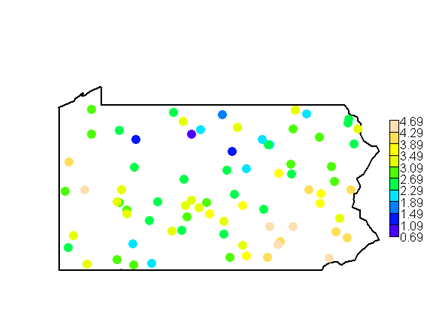
\includegraphics[height=2.75in]{figs/PA1}
\end{center}
\caption{Needs a caption}
\label{fig.PA1}
\end{figure}

We do have a measure of forest cover in the vicinity of each point which is contained in the data set (``habitat''). This was derived from a larger GIS coverage of the state (provided in the data file ``pahabdata'') which can be plotted using the spatial.plot function using the following commands
\begin{verbatim}
> map('state',regions="penn",lwd=2)
> spatial.plot(pahabdata[,2:3],pahabdata[,"dfor"],cx=2)
> map('state',regions="penn",lwd=2,add=TRUE)
\end{verbatim}


\begin{figure}
\begin{center}
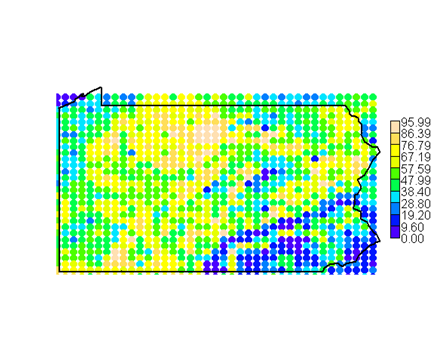
\includegraphics[height=2.75in]{figs/PA2}
\end{center}
\caption{Needs a caption}
\label{fig.PA21}
\end{figure}


We see a prominent pattern that indicates high forest coverage in the
central part of the state and low forest cover in the SE.  Inspecting
the previous figure of log-counts suggests a relationship between
counts and forest cover which is not surprising.

\subsection{Doing it in WinBUGS}
Here we demonstrate how to fit a Poisson GLM in WinBUGS using the covariate $x(i) =$ forest cover. It is advisable that $x(i)$ be standardized in most cases as this will improve mixing of the Markov chains. Recall that the data we have stored include a standardized covariate (forest cover) and so we don't have to worry about that here.  To read the BBS data into R and get things set up for WinBUGS we issue the following commands: 
\begin{verbatim}
data<-read.csv("pa-bbsdovedata-all.csv")
y<-data[,29]  # pick out 1990
notna<-!is.na(y)
y<-y[notna]
habitat<-data[notna,4]
library("R2WinBUGS")
data <- list ( "y","M","habitat")
\end{verbatim}
Now we write out the Poisson model specification in WinBUGS pseudo-code, provide initial values, identify parameters to be monitored and then execute WinBUGS:
\begin{verbatim}
cat("
model {
    for (i in 1:M){
      y[i]~dpois(lam[i])
      log(lam[i])<- beta0+beta1*habitat[i]
     }
 beta0~dunif(-5,5)
 beta1~dunif(-5,5)
}
",file="PoissonGLM.txt")

inits <- function()  list ( beta0=rnorm(1),beta1=rnorm(1))
parameters <- c("beta0","beta1")
out<-bugs (data, inits, parameters, "PoissonGLM.txt", n.thin=2, n.chains=2, n.burnin=2000,n.iter=6000,debug=TRUE,working.dir=getwd())
\end{verbatim}

{\bf Remarks:} (1) Note the close correspondence in how the model is specified here compared with the normal regression model previously. As an exercise you should discuss the specific differences between the BUGS model specifications for the normal and Poisson models.
\begin{verbatim}
> print(out,digits=3)
Inference for Bugs model at 
``PoissonGLM.txt'', fit using WinBUGS,
 2 chains, each with 4000 iterations (first 1000 discarded), n.thin = 2
 n.sims = 3000 iterations saved
             mean     sd     2.5%      25%      50%      75%    97.5%  Rhat n.eff
beta0       3.151  0.025    3.102    3.135    3.151    3.168    3.199 1.001  2300
beta1      -0.498  0.021   -0.539   -0.512   -0.498   -0.484   -0.457 1.001  3000
fit       869.930 19.856  835.500  855.700  868.600  881.900  913.602 1.002  1600
fitnew     76.709 12.519   54.098   68.107   76.215   84.510  102.602 1.001  3000
deviance 1116.605  2.014 1115.000 1115.000 1116.000 1117.000 1122.000
1.001  3000
\end{verbatim}


We might wonder whether this model provides an adequate fit to our data.  To evaluate that, we used a Bayesian p-value analysis with fit statistic based on the Freeman-Tukey residual by replacing the model specification above with this:

\begin{verbatim}
cat("
model {
    for (i in 1:M){
      y[i]~dpois(lam[i])
      log(lam[i])<- beta0+beta1*habitat[i]
      d[i]<-  pow(pow(y[i],0.5)-pow(lam[i],0.5),2)   #

      ynew[i]~dpois(lam[i])
      dnew[i]<-pow( pow(ynew[i],0.5)-pow(lam[i],0.5),2)

     }
 fit<-sum(d[])
 fitnew<-sum(dnew[])
 beta0~dunif(-5,5)
 beta1~dunif(-5,5)
}


",file="PoissonGLM.txt")
\end{verbatim}
The Bayesian p-value is the proportion of times $fitnew > fit$ which, for this data set, is 0, which was 1.0 in this case (calculation omitted). This suggests that the basic Poisson model does not fit well. 


\subsection{ Constructing your own MCMC algorithm}

It will be helpful for people to suffer through a couple examples building a custom MCMC algorithm. So, here, we build a basic one for the Poisson regression model using a Metropolis-within-Gibbs approach. First, we will assume that the two parameters have diffuse normal priors, say $[\alpha] = norm(0,100)$ and $[\beta]=norm(0,100)$.  We need to collect the relevant elements of the model which are the likelihood $[y|\alpha,\beta] = prod_{i} [y[i]|\alpha\beta] $ which is, mathematically, the product of the Poisson pmf evaluated at $y[i]$, given particular values of $\beta0$ and $\beta1$. The priors are $[\alpha]$ and $[\beta]$. We identify the full conditionals which are $[\alpha|\beta, y]$ and $[\beta|\alpha,y]$.  We use the all-purpose rule for constructing full conditionals to discover that:
\[
 [\alpha|\beta,y] propto [y|\alpha,\beta][\alpha] 
\]
\[
 [\beta|\alpha,y] propto [y|\alpha,\beta][\beta]
\]
Remember we could replace the ``propto'' with ``equals'' if we simply put $[y|\beta]$ or $[y|\alpha]$ in the denominator. But, in general, $[y|\alpha]$ or $[y|\beta]$ will be quite a pain to compute and, more importantly, it is a constant as far as the operative parameter (beta or alpha, respectively) goes so we can just as well ignore it because, recall, the MH acceptance probability will be the ratio of the ful-conditional evaluated at a candidate draw to that evaluated at the current draw. So, the denominator required to change $\propto$ to $=$ winds up canceling from the MH acceptance probability.  Here we will use the random walk candidate generator.  The ``Metropolis within Gibbs'' algorithm for a Poisson regression is remarkably simple:

%% Kimmy: test this R code out below and see what happens!

\begin{verbatim}I would break this code up into more lines and have objects called ``prior'' and ``prior.candidate'' and ``lambda'' and ``likelihood.candidate''. Annoying stuff that will make it easier for people to understand. Also, remind people that $lik*prior = exp(log(like)+log(prior))$. Lots of people have been running around in the woods for years with traps, and have forgotten math.

You could also mention that this is a random walk M-H. It would help lots of people out to see a non-symmetric proposal distribution, and the extra step needed to account for it.

# put random number seed here
out<-matrix(NA,nrow=1000,ncol=2)   # matrix to store the output
beta0<- -1                         # starting values
beta1<- -.8

# begin the MCMC loop ; do 1000 iterations
for(i in 1:1000){

# update the beta0 parameter
lik.curr<- sum(log(dpois(y,exp(beta0+beta1*habitat)))) 
prior.curr<- log(dnorm(beta0,0,100))
beta0c<-rnorm(1,beta0,.25)         # generate candidate
lik.cand<- sum(log(dpois(y,exp(beta0c+beta1*habitat))))
prior.cand<- log(dnorm(beta0c,0,100))
if(runif(1)< exp(lik.cand+prior.cand-lik.curr-prior.curr)) beta0<-beta0c

# update the beta1 parameter
lik.curr<- sum(log(dpois(y,exp(beta0+beta1*habitat)))) 
prior.curr<- log(dnorm(beta1,0,100))
beta1c<-rnorm(1,beta1,.25)
lik.cand<- sum(log(dpois(y,exp(beta0+beta1c*habitat)))) 
prior.cand<- log(dnorm(beta1c,0,100))
if(runif(1)< exp(lik.cand+prior.cand-lik.curr-prior.curr)) beta1<-beta1c
out[i,]<-c(beta0,beta1)             # save the current values
}
\end{verbatim}


\begin{figure}
\begin{center}
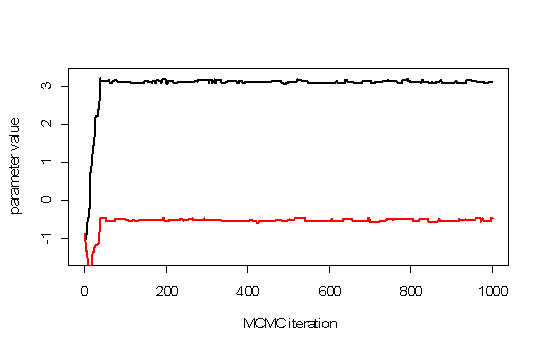
\includegraphics[height=2.75in]{figs/MCMC1}
\end{center}
\caption{Needs a caption}
\label{fig.MCMC1}
\end{figure}


Look at the output (beta0 in red, beta1 in black). You might not like the appearance of this output too much but a couple of things are evident: The Markov chains clearly stabilize - ``converge'' --  after about 100 iterations. They also appear to mix very slowly, although this is not so clear given the scale of the y-axis.
 

We decreased the variance for candidate generating distribution and
re-ran the MCMC algorithm producing the history plots below. We see
that the burn-in takes longer but it seems to mix better.


Fig. XYZ shows a longer MCMC run (10,000 total iterations) for beta1
based on discarding the first 400 samples as burn-in. The ``grassy''
look of the MCMC history is diagnostic of Markov chains that are
well-mixing.

\begin{figure}
\begin{center}
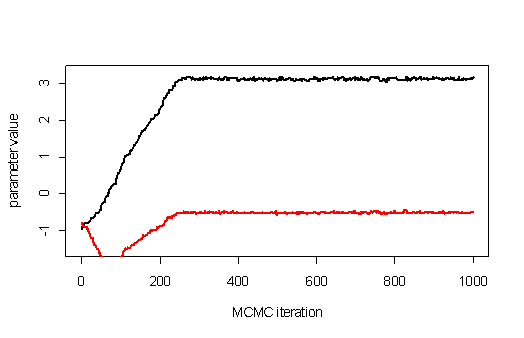
\includegraphics[height=2.75in]{figs/MCMC2}
\end{center}
\caption{Needs a caption}
\label{fig.MCMC2}
\end{figure}


\begin{figure}
\begin{center}
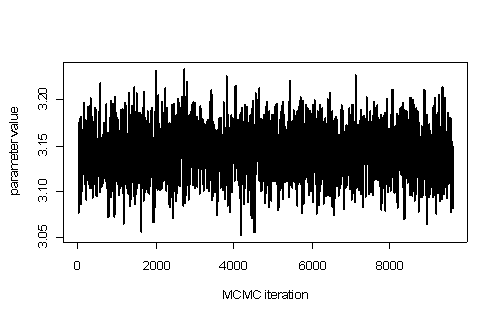
\includegraphics[height=2.75in]{figs/MCMC3}
\end{center}
\caption{Needs a caption}
\label{fig.MCMC3}
\end{figure}

{\bf Remarks:} We used a specific set of starting values for these
simulations. It should be clear that starting values closer to the
mass of the posterior distribution might cause burn-in to occur
faster. As an exercise, evaluate that.  (2) Clearly the influence of
the proposal variance term is important. Small values lead to much
better mixing but it should be noted that values that are too small
will lead to very slow mixing. We saw that values that were too large
tended to get the parameters stuck in one spot. This suggests there is
an optimal value of the Metropolis-Hastings tuning
parameter\footnote{Defined previously?}. As an exercise you should
find that optimal value. (3) For the flat normal prior distributions
here we could leave the prior contribution out of the full conditional
evaluation since it is ``locally constant''. Note also that we have
used a different prior than in our WinBUGS model specification. As an
exercise, evaluate whether this seems to affect the result.

\section{Poisson GLM with Random Effects}

What we will be doing in most of this book is dealing with random effects in GLM-like models - models that are usually referred to as generalized linear mixed models (GLMMs).

{\bf The Log-Normal mixture:} The classical situation involves a GLM with a normally distributed random effect. The linear predictor of the Poisson model is extended simply by adding a noise term, say:
\[
 	log(\lambda(i)) = \alpha  + \beta*x(i) + \eta[i]
\]
where $\eta[i]~normal(0,\sigma2)$.  A natural alternative is to have $exp(\eta[i])/\sim\gamma(a,b)$ which would correspond to a negative binomial kind of over-dispersion whereas the normal noise has a different mean/variance relationship (the interested reader should work that out).   Choosing between such possibilities is not a topic we will get into here because it doesn't seem possible to provide general guidance on it. Anyhow, it is really amazingly simple to express this model in WinBUGS and have WinBUGS draw samples from the posterior distribution using the following code for the BBS dove counts: 
\begin{verbatim}
data<-read.csv("pa-bbsdovedata-all.csv")
locs<-data[,2:3]
habitat<-data[,4]
y<-data[,29]
notna<-!is.na(y)  # to remove missing values
y<-y[notna]
locs<-locs[notna,]
habitat<-habitat[notna]
M<-length(y)

cat("
model {
            for (i in 1:M){
               y[i]~dpois(lam[i])
               log(lam[i])<- beta0+beta1*habitat[i] + eta[i]
               eta[i] ~ dnorm(0,tau)
               }
 beta0~dunif(-5,5)
 beta1~dunif(-5,5)
 sigma~dunif(0,10)
 tau<-1/(sigma*sigma)
}
\end{verbatim}
I have removed the final several R commands which package up the data and execute WinBUGS as those commands are largely redundant with the previous demo.  The summary results are:
\begin{verbatim}
> print(out,digits=3)
Inference for Bugs model at "model.txt", fit using WinBUGS,
 2 chains, each with 5000 iterations (first 1000 discarded), n.thin = 2
 n.sims = 4000 iterations saved
            mean     sd    2.5%     25%     50%     75%   97.5%  Rhat n.eff
beta0      2.967  0.076   2.817   2.915   2.969   3.020   3.111 1.006   430
beta1     -0.518  0.073  -0.657  -0.566  -0.517  -0.470  -0.374 1.008  4000
sigma      0.598  0.059   0.491   0.556   0.594   0.634   0.725 1.004   640
tau        2.883  0.569   1.904   2.489   2.836   3.233   4.149 1.004   640
fit       19.885  3.190  14.119  17.670  19.705  21.902  26.610 1.001  4000
fitnew    20.043  3.422  14.100  17.630  19.770  22.292  27.360 1.001  4000
deviance 446.255 12.290 424.000 437.700 445.600 454.100 472.302 1.001  4000

For each parameter, n.eff is a crude measure of effective sample size,
and Rhat is the potential scale reduction factor (at convergence, Rhat=1).

DIC info (using the rule, pD = Dbar-Dhat)
pD = 66.0 and DIC = 512.2
DIC is an estimate of expected predictive error (lower deviance is better).
> 

\end{verbatim}

The Bayesian p-value for this model is
\begin{verbatim}
> mean(out$sims.list$fit>out$sims.list$fitnew)
[1] 0.473
>
\end{verbatim}
indicating a pretty good fit. Given the site-level random effect, it
would be surprising for this model to not fit! One thing we notice is
that the posterior standard deviations of the regression parameters
are much higher, a result of the excess variation. (we would also
notice much less precise predictions of hypothetical new
observations).


\section{Binomial GLMs}

Another class of statistical models that are very important in ecology are binomial models. We use binomial models for count data whenever the observations are counts or frequencies and it is natural to condition on a ``sample size'' - the maximum frequency possible in a sample, say $K$ (i.e., $K$ is known). The random variable, $y/le K$, is then the frequency of occurrences out of $K$. The parameter of the binomial models is $p$, often called ``success probability'' which is related to the expected value of $y$ by $E[y] = pK$. Binomial GLMs or binomial regression models are often referred to as logistic regression, but that term really only applies when the logistic link is used to model the relationship between $p$ and covariates (see below).

One of the most typical Binomial GLMs occurs when the sample size
equals 1 and the outcome, $y$, is ``presence'' ($y=1$) or ``absence''
($y=0$) of a species. This is a classical ``species distribution''
modeling situation. A special situation occurs when presence/absence
is observed with error \citep{mackenzie_etal:2002,
  mackenzie_etal:2006, kery_etal:2010}. In that case, $K>1$ samples
are usually required in order to estimate model parameters
effectively. In standard binomial regression problems the sample size
is fixed by design but interesting models also arise when the sample
size is itself a random variable. These are the N-mixture models
\citep{royle:2004, kery_etal:2005, royle_dorazio:2008, kery:2010}
ch. 22) and related models (in this case, $N$ being the sample size
which we labeled K above). This is actually a little bit confusing
because the binomial index is usually referred to as ``sample size''
but in this context N is actually a ``population size''.  A useful
situation in which the binomial sample size is ``fixed'' is closed
population capture-recapture models in which a population of
individuals is sampled $K$ times.  The number of times each individual
is encountered is a binomial outcome with parameter - encounter
probability - $p$, based on a sample of size $K$.  We consider such
models in the following chapter.


\subsection{Binomial regression}

 In binomial models, covariates are modeled on a suitable transformation (the link function) of the binomial success probability, $p$.  Let  $x_{i}$ denote some measured covariate for sample unit $i$ and let $p_{i}$ be the success probability for unit i.  The standard choice is the ``logit'' link function which is:
\[
log(p[i]/(1-p[i])) = \alpha + \beta*x[i]
\]
with inverse ``expit''
\[
p[i] = expit(\alpha + \beta*x[i]) = exp(\alpha + \beta*x[i])/(1 + exp(\alpha + \beta*x[i])) 
\]
There are many other possible link functions. However, ecologists seem
to blindly adopt the logit link function without question to such an
extent that you are likely to be questioned by referees and associate
editors if you use some alternative link (unless you are doing species
distribution modeling, in which case any explicit link function will
be questioned by some referees).  We sometimes use the ``complementary
log-log'' (= ``cloglog'') link function in ecological applications
because it can often be justified based on subject-matter
considerations (\citet{royle_dorazio:2008}; section XYZ) or natural
scaling relationships germane to the problem.  For example, the
cloglog link arises as the ``probability of a count greater than 0''
under a Poisson model. That is, $\Pr(y>0) = 1-exp(- \lambda)$ in which case
\[
cloglog(p) =log(- log(1-p)) = log(\lambda)
\]
So that if you have covariates in your linear predictor for $E[y]$ under a Poisson model then they are linear on the complementary log-log link of p. We will use the cloglog link in some analyses of SCR models in Chapter 4 and elsewhere.  

A natural situation in which the cloglog link arises is modeling occupancy in which $N \sim Poisson(A*\lambda)$ and you have site area, A, measured for every sample. In this case the probability that the site is occupied, psi, is related to area on the cloglog scale. i.e.,
\[
 cloglog(\psi) = log(A) + log(\lambda).
\]
There seems to be perennial debate over whether site area should be a
covariate on ``detection'' or ``occupancy'' and the above argument
suggests the latter.


\subsection{ Example: Waterfowl Banding Data}

It would be easy to consider a standard ``distribution modeling''
application where $K=1$ and the outcome is occurrence ($y=1$) or not
($y=0$) of some species. Such examples abound in books (e.g.,
\citet{royle_dorazio:2008}, ch. 3; \citet{kery:2010}, chapter 21 XYZ?;
\citet{kery_schaub:2011}, chapter XYZ) and in the literature (see
\citet{kery_etal:2010}; \citet{kery_etal:2010} XYZ).  Instead, we will consider an example involving band returns of waterfowl which were analyzed by Royle and Dubovsky (200X)\footnote{not happy about this example. Anyone got a better one?}.  

For these data, $y[i]$ is the number of waterfowl bands recovered out of $B[i]$ birds banded at some location $s[i]$. In this case $B[i]$ is fixed. Thinking about recovery rate as being proportional to harvest rate, we wanted to explore geographic gradients in recovery rate resulting from variability in harvest pressure experienced by populations depending on their migration ecology. As such, we fit a basic binomial GLM with a linear response to geographic coordinates (including an interaction term). The data are provided on the web supplement along with an R script to do the post-processing. Here we just provide the part of the script for creating the model and calling WinBUGS:

\begin{verbatim}
sink("model.txt")
cat("
model {
 for(t in 1:5){
    for (i in 1:nobs){
       m[i,t] ~ dbin(p[i,t], R[i,t])
       logit(p[i,t]) <- alpha0[t] + alpha1*X[i,1] + alpha2*X[i,2] + alpha3*X[i,1]*X[i,2]
     }
}
	alpha1~dnorm(0,.001)
	alpha2~dnorm(0,.001)
	alpha3~dnorm(0,.001)
	for(t in 1:5){
 	alpha0[t] ~ dnorm(0,.001)  
 }
}
",fill=TRUE)
sink()

data <- list('R', 'm', 'nobs','X')
inits <- 	function(){
list(alpha0=rnorm(5),alpha1=0,alpha2=0,alpha3=0)
}
parms <- list('alpha0','alpha1','alpha2','alpha3')
out <- bugs(data,inits, parms,"model.txt",n.chains=3,
 					n.iter=2000,n.burnin=1000,
					n.thin=2, debug=TRUE)
\end{verbatim}

Posterior summaries of model parameters are as follows:

\begin{verbatim}
Inference for Bugs model at "model.txt", fit using WinBUGS,
 3 chains, each with 2000 iterations (first 1000 discarded), n.thin = 2
 n.sims = 1500 iterations saved
              mean    sd     2.5%      25%      50%      75%    97.5%  Rhat n.eff
alpha0[1]   -2.346 0.036   -2.417   -2.370   -2.346   -2.323   -2.277 1.001  1500
alpha0[2]   -2.356 0.032   -2.420   -2.379   -2.356   -2.335   -2.292 1.001  1500
alpha0[3]   -2.220 0.035   -2.291   -2.244   -2.219   -2.197   -2.153 1.001  1500
alpha0[4]   -2.144 0.039   -2.225   -2.169   -2.143   -2.116   -2.068 1.000  1500
alpha0[5]   -1.925 0.034   -1.990   -1.949   -1.924   -1.901   -1.856 1.004   570
alpha1      -0.023 0.003   -0.028   -0.025   -0.023   -0.022   -0.018 1.001  1500
alpha2       0.020 0.006    0.009    0.016    0.020    0.024    0.031 1.001  1500
alpha3       0.000 0.001   -0.002   -0.001    0.000    0.000    0.002 1.001  1500
deviance  1716.001 4.091 1710.000 1713.000 1715.000 1718.000 1726.000 1.001  1500

For each parameter, n.eff is a crude measure of effective sample size,
and Rhat is the potential scale reduction factor (at convergence, Rhat=1).

DIC info (using the rule, pD = Dbar-Dhat)
pD = 7.9 and DIC = 1723.9
DIC is an estimate of expected predictive error (lower deviance is better).
\end{verbatim}

The basic result suggests a negative east-west gradient and a positive south to north gradient but no interaction. A map of the response surface is given below. We could use DIC to do some model selection - i.e., try models without the interaction term, or models with a quadratic term, or with a constant intercept, etc., but we don't pursue that here. We did an MCMC run where we saved the binomial parameter p and computed the Bayesian p-value [double use of ``p'' here is confusing!] using a fit statistic based on the Freeman-Tukey statistic (see Section XXX above). The result indicates that the linear response surface model does not provide an adequate fit of the data. The reader should contemplate whether this invalidates the basic interpretation of the result.


\begin{figure}
\begin{center}
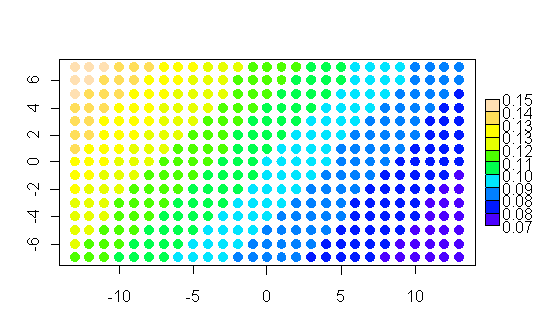
\includegraphics[height=2.75in]{figs/responsesurface}
\end{center}
\caption{Needs a caption}
\label{fig.responsesurface}
\end{figure}

\section{ Summary and Outlook}


GLMs and GLMMs are the most useful statistical methods in all of ecology. The principles and procedures underlying these methods are relevant to nearly all modeling and analysis problems in every branch of ecology. Moreover, understanding how to analyze these models is crucial in a huge number of diverse problems. If you understand and can conduct classical likelihood and Bayesian analysis of Poisson and binomial GLM(M)s, then you will be successful analyzing and understanding more complex classes of models that arise.We will see shortly that spatial capture-recapture models are just a type of GLMM (i.e., a GLM with a random effect) and thus having a basic understanding of the conceptual origins and formulation of GLMs and their analysis is extremely useful. We note that GLMs are routinely analyzed by likelihood methods but we have focused on Bayesian analysis here in order to develop the tools that are less familiar to most ecologists.  In particular, Bayesian analysis of GLMs with random effects (i.e., GLMMs) is relatively straightforward because the models are easy to analyze conditional on the random effect, using methods of MCMC.  Thus, we will often analyze SCR models in later chapters by MCMC, explicitly adopting a Bayesian inference framework.

In that regard, BUGS engines are enormously useful because they provides a straightforward way to carry out analyses by MCMC by just describing the model, and not having to worry about how to actually build MCMC algorithms.  That said, the BUGS language is more important than just to the extent that it enables one to do MCMC - it is useful as a modeling tool because it fosters understanding, in the sense that it forces you to become intimate with your model. You have to write down all of the probability assumptions, the relationships between observations and latent variables and parameters. This is really a great learning paradigm that you can grow with. Skills gained in Bayesian analysis of the GLMMs covered in this chapter will be directly transferrable and useful for the SCR models addressed subsequently. Before getting to that, however, it will be useful to talk about more basic, conventional closed population capture-recapture models and these are the topic of the next Chapter. 



%\chapter{Introduction}\label{chapt.intro}

%%\input{Chapter2-primer.tex}
%\input{Chapter3-uniformsearch.tex}
%\input{Chapter4-binomial.tex}
%\input{Chapter5-multistate.tex}

%\chapter{
Introduction to Bayesian Analysis of GL(M)Ms Using R/WinBUGS
}
\markboth{Chapter 2}{}
\label{chapt.intro}

\vspace{.3in}


A major theme of this book is that spatial capture-recapture models
are, for the most part, just generalized linear models (GLMs) wherein
the covariate, distance between trap and home range center, is
partially or fully unobserved  -- and therefore regarded as 
a random effect. Such models
are usually referred to as Generalized Linear Mixed Models (GLMMs)
and, therefore, SCR models can be thought of as a specialized type of
GLMM. Naturally then, we should consider analysis of these slightly
simpler models in order to gain some experience and, hopefully,
develop a better understanding of spatial capture-recapture models.

In this chapter, we consider classes of GLM models - Poisson and
binomial (i.e., logistic regression) GLMs - that will prove to be
enormously useful in the analysis of capture-recapture models of all
kinds. Many readers are probably familiar with these models because
they represent probably 
the most generally useful models in all of Ecology and, as
such, have received considerable attention in many introductory and
advanced texts. We focus on them here in order to introduce the
readers to the analysis of such models in {\bf R} and {\bf WinBUGS}, 
which we will
translate directly to the analysis of SCR models in subsequent
chapters.  

Bayesian analysis is convenient for analyzing GLMMs because it allows
us to work directly with the conditional model -- i.e., the model that
is conditional on the random effects, using computational methods
known as Markov chain Monte Carlo (MCMC). Learning how to do Bayesian
analysis of GLMs and GLMMs in {\bf WinBUGS} is, in part, the purpose
of this chapter.  While we use {\bf WinBUGS} to do the Bayesian
computations, we organize and summarize our data and execute {\bf
  WinBUGS} from within {\bf R} using the useful package \mbox{\tt
  R2WinBUGS} \citep{sturtz_etal:2005}.  \citet{kery:2010}, and
\citet{kery_schaub:2011} provide excellent introductions to the basics
of Bayesian analysis and GLMs at an accessible level. We don't want to
be too redundant with those books and so we avoid a detailed
treatement of Bayesian methodology - instead just providing a cursory
overview so that we can move on and attack the problems we're most
interested in related to spatial capture-recapture.  In addition,
there are a number of texts that provide general introductions to
Bayesian analysis, MCMC, and their applications in Ecology including
\citet{mccarthy:2007}, \citet{kery:2010}, \citet{link_barker:2009},and
\citet{king_etal:2009}.


While this chapter is about Bayesian analysis of GLMMs, such models
are routinely analyzed using likelihood methods too, as discussed by
\citet{royle_dorazio:2008}, and \citet{kery:2010}. Indeed, likelihood
analysis of such models is the primary focus of many applied
statistics texts, a good one being \citet{zuur_etal:2009}. Later in
this book, we will use likelihood methods to analyze SCR models but,
for now, we concentrate on providing a basic introduction to Bayesian
analysis because that is the approach we will use in a majority of
cases in later chapters.


\section{ Notation}

We will sometimes use conventional ``bracket notation'' to refer to
probability distributions. If $y$ is a random variable the $[y]$
indicates its distribution or its probability density/mass function
(pdf, pmf) depending on context. If $x$ is another random variable
then $[y|x]$ is the conditional distribution of $y$ given $x$, and
$[y,x]$ is the joint distribution of $y$ and $x$. To differentiate
specific distributions in some contexts we might label them $g(y)$,
$g(y|\theta)$, $f(x)$, or similar. We will also write $y \sim
\mbox{Normal}(\mu,\sigma^{2})$ to indicate that $y$ ``is distributed as'' a normal
random variable with parameters $\mu$ and $\sigma^{2}$. The expected value
or mean of a random variable is $E[y] = \mu$ ,and $Var[y] = \sigma^{2}$ is
the variance of $y$.  To indicate specific observations we'll use an
index such as ``$i$''. So, $y_{i}$ for $i=1,2,\ldots,n$ indicates
observations for $n$ individuals. Finally, we write $\Pr(y)$ to indicate specific probabilities, i.e., of events ``$y$'' or similar. 


To illustrate these concepts and notation, suppose $z$ is a binary
outcome (e.g., species occurrence) and we might assume the model: $z
\sim \mbox{Bern}(p)$ for observations.  Under this model $\Pr(z=1) =
\psi$, which is also the expected value $E[z] = \psi$. The variance is
$Var[z] = \psi*(1-\psi)$ and the probability mass function (pmf) is $[z]
= \psi^{z} (1-\psi)^{1-z}$. Sometimes we write $[z|\psi]$ when it is
important to emphasize the conditional dependence of $z$ on $\psi$. As
another example, suppose $y$ is a random variable denoting whether or
not a species is detected if an occupied site is surveyed. In this
case it might be natural to express the pmf of the observations $y$
{\it conditional} on $z$. That is, $[y|z]$. In this case, $[y|z=1]$ is
the conditional pmf of $y$ given that a site is occupied, and it is
natural to assume that $[y|z=1] = \mbox{Bern}(p)$ where $p$ is the
``detection probability'' - the probability that we detect the
species, given that it is present. The model for the observations $y$
is completely specified once we describe the other conditional pmf
$[y|z=0]$. For this conditional distribution it is sometimes
reasonable to assume $\Pr(y=1|z=0) = 0$ (\citet{mackenzie_etal:2002};
see also \citet{royle_link:2006}). That is, if the species is absent,
the probability of detection is 0. This implies that
$\Pr(y=0|z=0)=1$. To allow for situations in which the true state $z$
is unobserved, we  assume that $[z]$ is Bernoulli with parameter
$\psi$.  In this case, the marginal distribution of $y$ is
\[
 [y] = [y|z=1]Pr(z=1) + [y|z=0]Pr(z=0)
\]
because $[y|z=0]$ is a point mass at $y=0$, by assumption, then 
\[
\Pr(y=1) = p \psi
\]
And
\[
\Pr(y=0) = (1-p)*\psi + (1-\psi)
\]


\section{
GLMs and GLMMs}
We have asserted already that SCR models work out most of the time to
be variations of GLMs and GLMMs. Some of you might therefore ask: What
are GLMs and GLMMs, anyhow?   These models are covered extensively in
many very good applied statistics books and we refer the reader
elsewhere for a detailed introduction. We think \citet{kery:2010},
\citet{kery_schaub:2011}, and \citet{zuur_etal:2009} are all
accessible treatments of considerable merit. Here, we'll give the 1
minute 
treatment of GLMMs, not trying to be complete but rather only 
to preserve a coherent organization to the book.


The generalized linear model (GLM) is an extension of standard linear
models by allowing the response
variable to have some distribution from the exponential family of
distributions (i.e., not just normal). This includes the normal
distribution but also dozens of others such as the Poisson, binomial,
gamma, exponential, and many more. In addition, GLMS allow the
response variable to be related to the predictor variables (i.e.,
covariates) using a
link function, which is usually nonlinear.  Finally, GLMs typically
accommodate a relationship between the mean and variance. The
classical reference for GLMs is \citet{nelder_wedderburn:1972} and
also \citet{mccullagh_nelder:1989}.
The GLM consists of three components:
\begin{itemize}
\item[1.] A probability distribution for the dependent variable $y$, 
from a class of probability distributions known as the exponential family.
\item[2.] A ``linear predictor'' $\eta = {\bf X}{\bold \beta}$  . 
\item[3.] A link function $g$ that relates $E[y]$ to the linear predictor, $E[y] = \mu = g^{-1}(\eta)$. Therefore $g(E[y]) = \eta$.
\end{itemize}

The dependent variable $y$ is assumed to be an outcome from a
distribution of the exponential family which includes many common
distributions including the normal, gamma, Poisson, binomial, and many
others. The mean of the distribution of $y$ is assumed to depend on predictor variables $x$ according to 
\[
 g(E[y]) = {\bf x}'{\bold \beta}
\]
where $E[y]$ is the expected value of $y$, and ${\bf x}'{\bold \beta}$
is termed the {\it linear predictor}, i.e., a linear function of the
predictor variables with unknown parameters ${\bold \beta}$ to be
estimated.  The function $g$ is the link function. In standard GLMs,
the variance of $y$ is a function $V$ of the mean of $y$: $Var(y) =
V(\mu)$ (see below for examples).

A Poisson GLM posits that $y \sim \mbox{Poisson}(\lambda)$ with $E[y]
=\lambda$ and usually the model for the mean is specified using the
{\it log link function} by
\[
log(\lambda_{i}) = \beta_0 + \beta_{1}*x_{i}
\]
The variance function is $\mbox{V}(y_{i}) = \lambda_{i}$.  The
binomial GLM posits that $y_{i} \sim \mbox{Binomial}(K,p)$ where $K$
is the fixed sample size parameter and $E[y_{i}] = K*p_{i}$. Usually
the model for the mean is specified using the {\it logit link
  function} according to
\[
 logit(p_{i}) = \beta_{0} + \beta_{1}*x_{i}
\]
Where $logit(u) = log(u/(1-u))$.  The inverse-logit function, $g^{-1}$ ,
is a function we will refer to as ``expit'', so that $expit(u) =
exp(u)/(1+exp(u))$.

A GLMM is the extension of GLMs to accommodate ``random
effects''. Often this involves adding a normal random effect to the
linear predictor, and so a simple example is:
\[
 \log(\lambda_{i}) = \alpha_{i} + \beta_{1}*x_{i}
\]
where
\[
 \alpha_{i} \sim \mbox{Normal}(\mu,\sigma^{2})
\]
%Many other probability distributions and formulations of the linear
%predictor might be considered.  It is not widely appreicated that
%the link function and
%distribution of the random effect interact directly to affect the
%implied probability distribution of the linear predictor. For the
%Poisson case just considered, $\lambda_{i}$ has a log-normal
%distribution. However, if we set $\lambda_{i} = \alpha_{i}exp(\beta*x_{i})$
%where $\alpha_{i}$ has a Gamma distribution, then $\lambda_{i}$ has
%similarly a gamma distribution with modified scale parameter.  These
%different model assumptions are seldom evaluated formally in practice
%although in many practical situations (in ecology), they imply
%specific things about the ecological process being studied 
%(e.g., see \citet{royle_dorazio:2008} section XYZ on occupancy 
%logit/cloglog etc..).



\section{Bayesian Analysis}

Bayesian analysis is unfamiliar to many ecological researchers because older cohorts of ecologists were largely educated in the classical statistical paradigm of frequentist inference. But advances in technology and increasing exposure to benefits of Bayesian analysis are fast making Bayesians out of people or at least making Bayesian analysis an acceptable, general, alternative to classical, frequentist inference.  

Conceptually, the main thing about Bayesian inference is that it uses
probability directly to characterize uncertainty about things we don't
know.  ``Things'', in this case, are parameters of models and, just as
it is natural to characterize uncertain outcomes of stochastic
processes using probability, it seems natural also to characterize
information about unknown ``parameters'' using probability. At least
this seems natural to us and, we think, most ecologists either
explicitly adopt that view or tend to fall into that point of view
naturally. 
Conversely,
frequentists use probability in many different ways, but never to
characterize uncertainty about parameters\footnote{This will be
  shocking to most readers.}
It is paradoxical that people readily
adopt a philosophy of statistical inference in which the things you
don't know (i.e., parameters) should {\it not} be regarded as random
variables, so that, as a consequence, one cannot use probability to
characterize ones state of knowledge about them. 


\subsection{Bayes Rule}

As its name suggests, Bayesian analysis makes use of Bayes' rule in
order to make direct probability statements about model
parameters. Given two random variables $x$ and $y$, Bayes rule relates
the two conditional probability distributions $[x|y]$ and $[y|x]$ by the relationship:
\[
[x|y] = [y|x][x]/[y]
\]
Bayes' rule itself is a mathematical fact and there is no debate as to its validity and relevance to many problems. As an example of a simple application of Bayes rule, consider the problem of determining species presence at a sample location based on imperfect survey information. Let z be a binary random variable that denotes species presence $(z=1)$ or absence $(z=0)$, let $Pr(z=1) = psi$, and let $p$ be the probability that a species is detected in a single survey at a site given that it is present. If we survey a site $T$ times but never detect the species, then this clearly does not imply that the specie sis not present ($z=0$) at this site. Rather, our degree of belief in $z=0$ should be made with a probabilistic statement $Pr(z=1|y1=0,...,yT=0)$. If the $T$ surveys are independent so that we might regard $y_{t}$ as iid Bernoulli trials, then the total number of detections say $n$ is Binomial with probability $p$ then we can use Bayes rule to compute  the probability that it is present given that it is not detected in T samples as
\[
Pr(z=1|n=0) = Pr(n=0|z=1)Pr(z=1)/Pr(n=0) = [(1-p)^{T} psi]/[ (1-p)^T psi + (1-psi) ]
\]
({\bf It would be would be nice to label the different parts of this equation as to their analogy with Bayes' Rule... I know it sounds kind of basic, but I think it might be nice to see that explicitly. Maybe just say something like 'not detected (corresponding to the observation y in equation XX) , z=1 (corresponding to theta in eq. XX) and so on... }
For example, suppose that $T=2$ surveys are done at a wetland for a species of frog, and the species is not detected there. Suppose further that $psi = .8$ and $p = .5$ are obtained from a prior study.  Then the probability that the species is present at this site is  $.25*.8/(.25*.8 + .2) = 0.50$. That is, there seems to be about a 50/50 chance that the site is occupied despite the fact that the species wasn't observed there.

Bayes rule provides a simple linkage between the conditional probabilities $[y|x]$ and $[x|y]$ and no one disputes it as a basic fact of probability. 


\subsection{Bayesian Inference}


What is controversial to some is the scope and manner in which Bayes rule is applied by Bayesian analysts. Bayesian analysts assert that Bayes rule is relevant, in general, to all statistical problems by regarding all unknown quantities of a model as realizations of random variables - this includes ``data'', latent variables, and also ``parameters''. Classical (non-Bayesian) analysts sometimes object to regarding ``parameters'' as outcomes of random variables. Classically, parameters are thought of as ``fixed but unknown'' (using the terminology of classical statistics). Of course, in Bayesian analysis they are also unknown and, in fact, there is a single data-generating value and so they are also fixed. The difference is that this fixed but unknown value is regarded as having been generated from some probability distribution. Specification of that probability distribution is necessary to carryout Bayesian analysis.


To see the general relevance of Bayes rule in the context of statistical inference, let $y$  denote observations - i.e., ``data'' - and let $[y|\theta]$ be the observation model (often colloquially referred to as the ``likelihood'').  Suppose theta is a parameter of interest having (prior) probability distribution $[\theta]$. These are combined to obtain the posterior distribution using Bayes' rule, which is:
\[
 [\theta|y]= [y|\theta][\theta]/[y]
\]
Asserting the general relevance of Bayes rule to all statistical
problems, we can conclude that the two main features of Bayesian
inference are that: (1) ``parameters'' are regarded as realizations of
a random variable and, as a result, (2) inference is based on the
probability distribution of the parameters given the data, which is
called the posterior distribution. This is the result of using Bayes
rule to combine ``the likelihood'' and the prior distribution.  The
key concept is regarding parameters as realizations of a random
variable because, once you admit this conceptual view, this leads
directly to the posterior distribution, a very natural quantity upon
which to base inference about things we don't know -  including parameters of statistical models.  


We note that the denominator of our invocation of Bayes rule, $[y]$, is the marginal distribution of the data $y$.   We note without further remark right now that, in many practical problems, this can be an enormous pain to compute. The main reason that the Bayesian paradigm has become so popular in the last 20 years or so is because methods exist for characterizing the posterior distribution that do not require that we possess a mathematical understanding of $[y]$, i.e., we never have to compute it or know what it looks like, or know anything specific about it. 


A common misunderstanding on the distinction between Bayesian and frequentist inference goes something like this ``in frequentist inference parameters are fixed but unknown but in a Bayesian analysis parameters are random.'' At best this is a sad caricature of the distinction and at worst it is downright wrong. What is true is that, to a Bayesian, parameters are random variables. However, a Bayesian assumes, just like a frequentist, that there was a single data-generating value of that parameter - a fixed, and unknown value.  The distinction between Bayesian and frequentist approaches is that Bayesians regard the parameter as a random variable, and its value as the outcome of a random value, on par with the observations. This allows Bayesians to use probability to make direct probability statements about parameters. Frequentist inference procedures do not permit direct probability statements to be made about parameter values- because parameters are not random variables!

While we can understand the conceptual basis of Bayesian inference
merely by understanding Bayes rule -1 that's really {\it all there is
  to it} - it is not so easy to understand the basis of  classical
``frequentist'' inference which is really ``a basket of methods'' with
little coherent organization. What is mostly coherent in frequentist
inference is the manner in which items in this ``basket of methods''
are evaluated - the performance of a given procedure is evaluated by
``averaging over'' hypothetical realizations of $y$. This leads to
interpretations that are not so straightforward. For example
confidence intervals having the interpretation ``95\% probability that the interval contains the true value" and p-values being "the probability of observing an outcome as extreme or more than the one observed''. Moreover, this is conceptually probblematic to some because the hypothetical realizations that characterize the performance of our procedure we will never get to observe.  

That said,  we advocate for a pragamatic non-partisian approach to inference because, frankly,  some of these ``bucket of methods'' are actually very convenient in certain situations as we will see in later chapters.


\subsection{Prior distributions}
{\bf It would be nice to explain at some point what a prior can look like/where it can come from, what informative/uninformative means... I though further down the chapter that there was quite a bit of explanation on the posterior, but then you kind of just jump into choosing priors, which, for someone who may not really ever have done a Bayesian analysis, might be a little puzzling }

An oft-touted benefit of Bayesian analysis is the ease with which
prior information can be included. The manner in which this happens is
usually largely subjective, but still the need arises from time to
time. In SCR models we often have a parameter that is closely linked
to ``home range radius'' and thus auxiliary information on the home
range size of a species can be used as prior information (e.g., see
\citet{chandler_royle:2012} ; also chapter XYZ). 



\subsection{Posterior Inference}

Posterior inference is the main practical element  of Bayesian analysis. We get to make an inference conditional on the data that we actually observed - i.e., what we actually know.  To us, this seems logical - to condition on what we know. Conversely, frequentist inference is based on considering average performance over hypothetical unobserved data sets (i.e., the ``relative frequency'' interpretation of probability).  Frequentists know that their procedures work well when averaged over all hypothetical, unobserved, data sets but no one ever really knows how well they work for the specific data set analyzed. That seems like a relevant question to biologists who oftentimes only have their one, extremely valuable, data set.
This distinction comes into play a lot in exposing philosophical biases in the peer review of statistical analyses in ecology in the sense that, despite these opposing conceptual views to inference (i.e. conditional on the data you have, or averaged over hypothetical realizations), those who conduct a Bayesian analysis are often required to provide a frequentist evaluation of their Bayesian procedure.  

  It is worth emphasizing that, in Bayesian inference, we are not focusing on estimating a single point or interval but rather characterizing a whole distribution from which one can report any summary of interest. A point estimate might be the posterior mean, median, mode, etc..  In many applications in this book, we will compute 95% Bayesian intervals using the 2.5% and 97.5% quantiles of the posterior distribution. For such intervals, it is correct to say $Pr(L < theta < U) = 0.95$. That is, "the probability that theta is between L and U is 0.95". It is not a subtle thing that this cannot be said using frequentist methods - although people tend to say it anyway and not really understand why it is wrong or even that it is wrong. This is actually a failing of frequentist ideas and the inability of frequentists to get people to overcome their natural tendency to use probability - which is something that, as a frequentist, you simply cannot do in the manner that you would like to.  



\subsection{Small sample inference}
Using Bayesian inference, we obtain an estimate of the posterior distribution which is an exhaustive summary of the state-of-knowledge about an unknown quantity. It is the posterior distribution - not an estimate of that thing. It is also not, usually, an approximation except to within Monte Carlo error (in cases where we use simulation to calculate it).  One of the great virtues of Bayesian analysis which is not really appreciated is that it is completely valid for any particular sample size. i.e., $[theta|y$ is, as precise as we claim it to be, for the particular sample size and observations that we have.  The same cannot be said for almost all frequentist procedures in which estimates or variances are very often based on ``asymptotic approximations'' to the procedure which is actually being employed.  

There seems to be a prevailing view in statistical ecology that classical likelihood-based procedures are virtuous because of the availability of simple formulas and procedures for carrying out inference, such as calculating standard errors, doing model selection by AIC, and assessing goodness-of-fit.  In large samples, this may be an important practical benefit, but the practical validity of these procedures cannot be asserted in most situations involving small samples.  This is not a minor issue because it is typical in many wildlife sampling problems - especially in surveys of carnivores or rare/endangered species - to wind up with a small, sometimes extremely small, data set. For example, a recent paper on the fossa (Cryptoprocta ferox), an endangered carnivore in Madagascar, estimated an adult density of 0.18 adults / km sq based on 20 animals captured over 3 years \citep{hawkins_racey:2005}. A similar paper on the endangered southern river otter (Lontra provocax) estimated a density of 0.25 animals per river km based on 12 individuals captured over 3 years \citep{sepulveda_etal:2007}. \citet{gardner_etal:2010} analyzed data from a study of the Pampas cat, a species for which very little is known, wherein only 22 individual cats were captured .during the two year period.  \citet{trolle_kery:2005} reported only 9 individual ocelots captured and \citet{jackson_etal:2006} captured 6 individual snow leopards using camera trapping. Thus, studies of rare and/or secretive carnivores necessarily and flagrantly violate one of Le Cam's Basic Principles, that of ``If you need to use asymptotic arguments, do not forget to let your number of observations tend to infinity.''\citep{lecam:1990}.

The biologist thus faces a dilemma with such data. On one hand, these datasets, and the resulting inference, are often criticized as being poor and unreliable. Or, even worse\footnote{Actual quote from a referee}, ``the data set is so small, this is a poor analysis.''  On the other hand, such data may be all that is available for species that are extraordinarily important for conservation and management.    The Bayesian framework for inference provides a valid, rigorous, and flexible framework that is theoretically justifiable in arbitrary sample sizes. This is not to say that one will obtain precise estimates of density or other parameters, just that your inference is coherent and justifiable from a conceptual and technical statistical point of view. That is, we report the posterior probability $Pr(D|data)$ which is easily interpretable and just what it is advertised to be and we don't need to do a simulation study to evaluate how well some approximate $Pr(D|data)$ deviates from the actual $Pr(D|data)$ because they are precisely the same quantity.



\section{Characterizing posterior distributions by MCMC simulation}  

In practice, it is not really feasible to ever compute the marginal probability distribution $Pr(y)$, the denominator resulting from application of Bayes' rule. For decades this impeded the adoption of Bayesian methods by practitioners. Or, the few Bayesian analyses done were based on asymptotic normal approximations to the posterior distribution. While this was useful stuff from a theoretical and technical standpoint and, practically, it allowed people to make the probability statements that they naturally would like to make, it was kind of a bad joke around the Bayesian water-cooler to, on one hand, criticize classical statistics for being, essentially, completely ad hoc in their approach to things but then, on the other hand, have to devise various approximations to what they were trying to characterize. The advent of Markov chain Monte Carlo (MCMC) methods has made it easier to calculate posterior distributions for just about any problem to arbitrary levels of precision.  

Broadly speaking, MCMC is a class of methods for drawing random numbers (sampling or simulating) from the target posterior distribution.  Thus, even though we might not recognize the posterior as a named distribution or be able to analyze its features analytically, e.g., devise mathematical expressions for the mean and variance, we can use these MCMC methods to obtain a large sample from the posterior and then use that sample to characterize features of the posterior. What we do with the sample depends on our intentions -- typically we obtain the mean or median for use as a point estimate, and take a confidence interval based on Monte Carlo estimates of the quantiles.  These are estimates, but not like frequentist estimates. Rather, they are Monte Carlo estimates with an associated Monte Carlo error which is largely determined arbitrarily by the analyst. They are not estimates qualified by a sampling distribution as in classical statistics. If we run our MCMC long enough then our reported value of $E[theta|y]$ or any feature of the posterior distribution is precisely what we say it is. There is no ``sampling variation'' in the frequentist sense of the word.  In summary, the MCMC samples provide a Monte Carlo characterization of {\it the} posterior distribution.


\section{What Goes on Under the MCMC Hood}

A type of MCMC method relevant to most problems is Gibbs sampling, which is based on the idea of iterative simulation from the ``full conditional'' distributions (also called conditional posterior distributions). The full conditional distribution for an unknown quantity is the conditional distribution of that quantity given every other random variable in the model - the data and all other parameters. For example, for a normal regression model with $y \sim Normal(alpha + beta*x , 1)$ then the two full conditionals are, in symbolic terms,
\[ 
[\alpha|y,\beta]
\]
 and 
\[
[\beta|y,\alpha]
\]. 
We might use our knowledge of probability to identify these mathematically. In particular, by Bayes' Rule, [alpha|y,beta] = [y|alpha,beta][alpha|beta]/[y|beta] and similarly for [beta|y,alpha]. For example, if we have priors for [alpha] and [beta] which are also normal distributions, some algebra reveals that 
\[
[\alpha|y,\beta] = Normal(ybar,...weighted variance here...). 
\]
Similarly,
\[
 [\beta|y,\alpha] is normal(........) 
\]

Thus, the MCMC algorithm has us simulate successively and repeatedly from those two distributions. See Gilks et al. (MCMC in practice book REF XXXX) for more examples with the normal model. A conceptual representation of the MCMC algorithm for this simple model is therefore: 
\begin{verbatim}
Algorithm:

0.	Initialize $\alpha$ and $\beta$

Repeat{
1.	Draw a new value of $\alpha$ from Eq. \ref{xyz}

2.	Draw a new value of $\beta$ from Eq. \ref{xyz}
}
\end{verbatim}

As we just saw for this simple ``normal-normal'' model it is sometimes possible to specify the full conditional distributions analytically. In general, when certain so-called conjugate prior distributions are chosen, the form of full conditional distributions is similar to that of the observation model. In this normal-normal case, choice of normal priors for the mean parameters is the conjugate prior under the normal model, and thus the full-conditional distributions are also normal. This is convenient because, in such cases, we can simulate directly from them using standard methods (or R functions).  But, in practice,  we don't really ever need to know such things because most of the time we can get by using a simple algorithm, called the Metropolis-Hastings (henceforth ``MH'') algorithm, to obtain samples from these full conditional distributions without having to recognize them as specific, named, distributions. As we noted above, this gives us enormous freedom in developing models and analyzing them without having to resolve them mathematically because to implement the MH algorithm   we need only identify the full conditional distribution up to a constant of proportionality, that being the marginal distribution in the denominator (e.g., $[y|beta]$ above).


\subsection{Rules for constructing full conditional distributions}  

The basic strategy for constructing full-conditional distributions for devising MCMC algorithms can be reduced conceptually to a couple of basic steps summarized as follows:
\begin{itemize}
\item[(step 1)] collect all stochastic components of the model; 
\item[(step 2)] Recognize and express the full conditional in question as proportional to the product of all  components; 
\item[(step 3)] remove the ones that don't have the focal parameter in them. 
\item[(step 4)] Do some algebra on the result in order to identify the resulting pdf or pmf. 
\end{itemize}
Of the 4 steps, the last of those is the main step that requires quite a bit of statistical experience and intuition because various algebraic tricks can be used to reshape the mess into something noticeable - i.e., a standard, named distribution. But step 4 is not necessary if we decide instead to use the Metrpolis-Hastings algorithm as described below. 

% KIMMY: dollar-signs around everything with a bracket please! Also convert to \alpha
% \beta for greek letters

To illustrate for computing $[\alpha|y,\beta]$ we first apply step 1 and identify the model components as $[y|\alpha, \beta]$, $[\alpha]$ and $[\beta]$. Step 2 has us write $[\alpha|y,\beta] \propto [y|\alpha,\beta][\alpha][\beta]$.  We note that $[\beta]$ is not a function of alpha and therefore we delete it to get $[\alpha|y,\beta] \propto [y|\alpha,\beta][\alpha]$. Similarly we get $[\beta|y,\alpha] \propto [y|\alpha,\beta][\beta]$. We can apply step 4 and manipulate these algebraically to arrive at the result or, alternatively, we can sample them indirectly using the Metropolis-Hastings algorithm (see below).   


\subsection{Metropolis-Hastings algorithm}
 
The Metropolis-Hastings algorithm is a completely generic method for
sampling from any distribution, say $f(\theta)$. In our applications,
$f(theta)$ will typically be the full conditional distribution for
theta. Often, the MH algorithm is used to sample from the full
conditional distributions and the resulting synthetic algorithm is
called ``Metropolis within Gibbs'' or similar. Shortly we will
actually construct such an algorithm for a simple class of models.
The Metropolis-Hastings algorithm generates candidates from some
proposal or candidate-generating distribution, that may be conditional
on the current value of the parameter, denoted by
$h(theta|theta^{current})$. Then you accept the proposed value with
probability
\[
f(\theta^{cand}) h(\theta^{current}|\theta^{cand})/
f(\theta^{current}) h(\theta^{cand}|\theta^{current})
\]
this ratio can sometimes be $>1$ in which case we set it equal to
1. It is useful to note that $h()$ can be anything at all. Absolutely anything!  You can generate candidate values from a $normal(0,1)$ distribution, from a uniform(-3455,3455) distribution, or anything of proper support.  Note, however, that good choices of $h()$ are those that approximate the posterior distribution. Obviously if $h() = f(\theta|y)$ (i.e., the posterior) then you always accept the draw, and it stands to reason that proposals that are more similar to $f(\theta|y)$ will lead to higher acceptance probabilities. No matter the choice of $h()$,  we can evaluate this ratio numerically because the marginal $f(y)$ cancels from both the numerator and denominator. (That is kind of the magic point here that I should emphasize better above.) 

A special kind of $h()$ are those that are symmetric, which means that $h(a|b) = h(b|a)$ in which case $h(a|b)$ and $h(b|a)$ just cancel out. A type of symmetric proposal useful in many situations is the so-called ``random-walk'' proposal distribution where candidate values are drawn from a normal distribution with mean equal to the current value and some standard deviation, say delta which is prescribed by the user. For parameters that have support on the real line, say alpha in our example above, the random walk proposal generator has us generate $alpha^{*} ~ Normal(alpha^{current},delta)$.  If we set delta very small we have a high probability of accepting the proposal and vice versa.  In practice, we ``tune'' delta to achieve a compromise between reasonable mixing of the Markov chains (see below for an example).

Parameters with bounded support: Many models contain parameters that have a bounded support. E.g., variance parameters live on $[0,\infty]$ or similar. In that case it is sometimes convenient to use a random walk proposal distribution, but just reject parameters that are outside of the parameter space (REF FOR THIS?). 



\section{Practical Bayesian Analysis and MCMC}

There are a number of really important practical issues to be considered in any Bayesian analysis and we cover some of these briefly here.

Prior distributions: Bayesian analysis requires that we choose prior
distributions for all of the structural parameters of the model (we
use the term structural parameter to mean all parameters that aren't
customary thought of as latent variables). We will strive to use
priors that are meant to express little or no prior information -
default or customary ``non-informative'' or diffuse priors. This will be uniform(a,b) priors for parameters that have a natural bounded support and, for parameters that live on the real line we use either (1) diffuse normal priors; (2) ``improper'' uniform priors or (3) sometimes even a bounded uniform(a,b) prior if that greatly improves the performance of WinBUGS or other software doing the MCMC for us.  In WinBUGS a prior with low ``precision'' (precision = 1/sigma2) such as normal(0,.01) will typically be used. Of course tau = 0.01 (sigma2 = 100) might be very informative for a regression parameter that has a high variance. Therefore, we recommend that predictor variables {\it always} be standardized. Clearly  there are a lot of choices for ostensibly non-informative priors, and the degree of non-informativeness depends on the parameterization. For example, a natural non-informative prior for the intercept of a logistic regression
\[
logit(p[i]) = a + b*x[i]
\]
Would be $[a] = const$ which is the same as saying $a \sim Unif(\infty,infty)$ or the standard improper ``locally uniform'' prior distribution.  However, we might also use a prior on the parameter $p0 = expit(a)$, which is $Pr(y=1)$ for the value $x=0$. Since $p0$ is a probability we might use $p0 \sim Unif(0,1)$. These two priors can affect results (see Chapter 3.XYZ), yet they are both sensible ``non-informative'' priors. Choice of priors and parameterization is very much problem-specific and often largely subjective. Moreover, it also affects the behavior of MCMC algorithms and therefore the analyst needs to pay some attention to these issues and possibly try different things out. [we should point to some standard refs on this stuff].

Once we have carried-out an analysis by MCMC, there are many other practical issues that we have to confront.  One of the most important is ``Have the chains converged?'' Most MCMC algorithms only guarantee that, eventually, the samples being generated will be from the target posterior distribution. So-called ``convergence'' of the Markov chain is achieved when that happens.  Typically a period of transience is observed in the early part of the MCMC algorithm, and this is usually discarded as the ``burn-in'' period.  

The quick diagnostic to whether convergence has been achieved is that
your Markov chains look ``grassy'' - see Figure XXX below - then
you're probably all done. Another way to check convergence is to
update the parameters some more and see if the posterior changes. It
is good to confirm convergence using the Rhat statistic (Brooks Gelman
Rubin statistic \citep{gelman_etal:1996}) which should be close to 1. In practice, 1.2 is probably good enough. For some really complex models 1.3 or 1.4 might be good enough. For some models you can't actually realize a low R-hat. E.g., if the posterior is a discrete mixture of distributions then I think you will always be misled into thinking that your Markov chains have not converged when in fact the chains are just jumping back and forth in the posterior state-space. Another situation is when one of the parameters is on the boundary of the parameter space which might appear to be very poor mixing. This kind of stuff is normally ok and you need to think really hard about the context of the model and the problem before you conclude that your MCMC algorithm is ill-behaved or not.

Some models exhibit ``poor mixing'' of the Markov chains or what
people might also call ``slow convergence'' which is a term we would
disagree with because the samples might well be from the posterior
(i.e., the Markov chains have converged to the proper stationary
distribution) but simply mix around the posterior rather
slowly. Anyway, poor mixing can happen for a huge number of reasons -
when parameters are highly correlated (even confounded), or barely
identified from the data, or the algorithms are very terrible and
probably many other reasons.  Slow mixing equates to high
autocorrelation in the Markov chain - the successive draws are highly
correlated, and thus we need to run the MCMC algorithm much longer to
get an effective sample size that is sufficient for estimation - or to
reduce the MC error to a tolerable level.  A strategy often used to
reduce autocorrelation is ``thinning'' - i.e., keep every $m^{th}$
value of the Markov chain output. However, thinning is necessarily
inefficient from the stand point of inference - you can always get
more precise posterior estimates by using all of the MCMC output
regardless of the level of autocorrelation \citep{maceachern_berliner:1994}. Practical considerations might necessitate thinning, even though it is statistically inefficient. For example, in models with many parameters or other unknowns being tabulated, the output files might be enormous and unwieldy to work with. In such cases, thinning is perfectly reasonable. In many cases, how well the Markov chains mix is strongly influenced by parameterization, standardization of covariates, and the prior distributions being used. Some things work better than others, and the investigator should experiment with different settings and try not to become bewildered when things don't work out perfectly. MCMC is an art, and a science. 


The next question: Is the posterior sample large enough?  Never report MCMC results to more than 2 decimal places - because they will always be different! Look at the MC error which is printed by default in *BUGS summaries.  You want that to be smallish relative to the magnitude of the parameter. I'm usually content with 1\% but if you're uncomfortable with monte carlo error, you should run your MCMC algorithm as long as it takes. Note that MC error in summaries of the posterior is not the same as having an ``approximate'' solution in a standard likelihood analysis or similar.  The approximate SE in likelihood inference is actually wrong in its actual value.... XYZ.


\subsection{Bayesian confidence intervals} 
The 95\% Bayesian interval based on percentiles of the posterior
is not a unique interval - there are many of them - and the so-called
``highest posterior density'' (HPD) interval is the narrowest
interval. We might compute that frequently because it is easy to do
with an integer parameter which $N$ is (See the next chapter). The
95p\% HPD is not often exactly 95\% but usually slightly more
conservative than nominal because it is the narrowest interval that
contains at least 95\%  of the posterior mass.

\subsection{Estimating functions of parameters} A benefit of analysis by MCMC is that we can seamlessly estimate functions of parameters by simply tabulating the desired function of the simulated posterior draws. For example, if $\theta$ is the parameter of interest and let $\theta^{(i)}$ for $i=1,2,\ldots,M$ be the posterior samples of $\theta$. Let $\eta = exp(\theta)$, then a posterior sample of $\eta$ can be obtained simply by computing $exp(\theta^{(i)})$ for $i=1,2,\ldots,M$. We give an example in Section XXXX below.


\section{Bayesian Analysis using WinBUGS}

We won't be too concerned with devising our own MCMC algorithms although we will do that one or two times for fun.  More often, we will rely on the freely available software package WinBUGS or other BUGS engines for doing this.  Further, we will execute WinBUGS from within R using the R2WinBUGS package. WinBUGS is an MCMC black box that takes a pseudo-code description of all of the relevant stochastic and deterministic elements of a model and generates an MCMC algorithm for that model. But you never get to see the algorithm. Instead, WinBUGS will run the algorithm and just return the Markov chain output - the posterior samples of model parameters. 

The great thing about WinBUGS is that it forces you to become intimate
with your statistical model - you have to write each element of the
model down, admit (explicitly) all of the various assumptions,
understand what the actual probability assumptions are and how data
relate to latent variables and data and latent variables relate to
parameters, and how parameters relate to one another. While we will
use WinBUGS almost exclusively here, there are many BUGS like packages
now, including JAGS, OpenBUGS, PyMC and others.  Later (chapter MCMC
XYZ) we will demonstrate a model or two in JAGS. OpenBUGS is the
current active development tree of the ``BUGS'' language. See
(\citet{kery:2010}; chapters XXXX) and (\citet{kery_schaub:2011}, Appendix XYZ) for the lowdown on problems/issues with using WinBUGS. That book should also be consulted for a more comprehensive introduction to using WinBUGS. In this example, we're going to accelerate pretty fast.

We  provide a brief introductory example of a normal regression model using a small simulated data set. The following commands are executed from within your R workspace, the command line being indicated by ``>''. First, simulate a covariate x and observations y having prescribed intercept, slope and variance:
\begin{verbatim}
> x<-rnorm(10)
> mu<- -3.2+ 1.5*x
> y<-rnorm(10,mu,sd=4)
\end{verbatim}
The WinBUGS model specification for a normal regression model is written within R as a character string input to the command cat() and then dumped to a text file named ``normal.txt'' (alternatively, you can write the model specifications directly within a text file and save it in your current working directory):
\begin{verbatim}
> cat("
model {
   for (i in 1:10){
      y[i]~dnorm(mu[i],tau)             # the "likelihood"
      mu[i]<- beta0 + beta1*x[i]   # the linear predictor
     }
   beta0~dnorm(0,.01)                   # prior distribution
   beta1~dnorm(0,.01)
   sigma~dunif(0,100)
   tau<-1/(sigma*sigma)                 # tau is a derived parameter
}
",file="normal.txt")
\end{verbatim}



{\bf Remarks:}
\begin{itemize}
\item[1.]WinBUGS parameterizes the normal in terms of the mean and inverse-variance, called the precision. Thus, dnorm(0,.01) implies a variance of 100.
\item[2.]We typically use diffuse normal priors for mean parameters, beta0 and beta1 in this case, but sometimes we might use uniform priors with suitable bounds -B and +B.
\item[3.]We typically use a uniform [0,B] prior on standard deviation parameters (Gelman XXX 2006). But sometimes we might use a gamma prior on the precision parameter tau.
\item[4.]In a WinBUGS model file, every single element has to be either data which will be input (see below), a random variable which must have a probability distribution associated with it, using the ``~'', or it has to be a derived parameter connected to variables and data using ``<-''.

\end{itemize}

To fit the model, we execute these commands:
\begin{verbatim}
> library("R2WinBUGS")    # "attach" the R2WinBUGS library
> data <- list ( "y","x")
> inits <- function()
  list ( beta1=rnorm(1),beta0=rnorm(1),sigma=runif(1,0,2) )
> parameters <- c("beta0","beta1","sigma","tau")
> out<-bugs (data, inits, parameters, "normal.txt", n.thin=2, n.chains=2, n.burnin=2000, n.iter=6000, debug=TRUE,working.dir=getwd())
\end{verbatim}
To fit the model, we execute these commands:
\begin{verbatim}
> library("R2WinBUGS")    # "attach" the R2WinBUGS library
> data <- list ( "y","x")
> inits <- function()
  list ( beta1=rnorm(1),beta0=rnorm(1),sigma=runif(1,0,2) )
> parameters <- c("beta0","beta1","sigma","tau")
> out<-bugs (data, inits, parameters, "normal.txt", n.thin=2, n.chains=2, n.burnin=2000, n.iter=6000, debug=TRUE,working.dir=getwd())
\end{verbatim}

{\bf Explanation:} We created an R list object called ``data'' which are the things we have to send to WinBUGS.  In the example above, the data consist of two objects which exist as ``y'' and ``x'' in the R workspace and also in the WinBUGS model definition.  People tend to ask ``how should my data be formatted?'' That depends on how you describe the WinBUGS model and you should read your data in as a .csv file or some other format and manipulated it within R to get into the desired format. There is a non-unique way to describe any particular model and so you have some flexibility. We talk about data format further in the context of capture-recapture models and SCR models in chapters 3 and 4, and later.  We also have to create an R function that produces a list of starting values ``inits'' that get sent to WinBUGS. In general, starting values are optional but we recommend to always provide reasonable starting values of structural parameters, but not necessarily random effects(although the latter will sometimes need to be given to keep WinBUGS from crashing).  Finally, we identify the names of the parameters (labeled correspondingly in the WinBUGS model specification) that we want WinBUGS to save the MCMC output for. In the above example, we are telling WinBUGS to ``monitor'' beta0, beta1, sigma and tau. WinBUGS is executed using the R command ``bugs''. Note that the previously created objects defining data, initial values and parameters to monitor are passed to this function. In addition, various other things are declared: The number of chains, the thinning rate, the number of burnin iterations and the total number of iterations. We set ``debug=TRUE'' if we want the WinBUGS GUI to stay open (useful for analyzing MCMC output and looking at the WinBUGS error log). Also, we set working.dir=getwd() so that WinBUGS output files and the log file are saved in the current R working directory.


You should execute all of the commands given above and then look at the resulting output. Kill the WinBUGS GUI and the data will be read back into R.  We don't want to give instructions on how to navigate and use the GUI - see REF (XYZ) for that.  The object ``out'' prints important summaries by default (this is slightly edited):

\begin{verbatim}
> print(out,digits=2)
Inference for Bugs model at "normal.txt", fit using WinBUGS,
 2 chains, each with 6000 iterations (first 2000 discarded), n.thin = 2
 n.sims = 4000 iterations saved
          mean   sd  2.5%   25%   50%   75% 97.5% Rhat n.eff
beta0    -2.43 1.84 -6.21 -3.50 -2.42 -1.34  1.27    1  4000
beta1     2.62 1.54 -0.42  1.68  2.62  3.57  5.67    1  4000
sigma     5.29 1.66  3.11  4.14  4.95  6.05  9.39    1  4000
tau       0.05 0.02  0.01  0.03  0.04  0.06  0.10    1  4000
deviance 59.85 3.24 56.18 57.47 59.00 61.37 68.32    1   840

For each parameter, n.eff is a crude measure of effective sample size,
and Rhat is the potential scale reduction factor (at convergence, Rhat=1).

DIC info (using the rule, pD = Dbar-Dhat)
pD = 2.6 and DIC = 62.4
\end{verbatim}

{\bf Remarks:} (1) convergence is assessed using the $\hat{R}$ statistic - which we will write ``Rhat''. A value of Rhat near 1 indicates convergence. Posterior summaries are given.  (2) DIC is the ``deviance information criterion'' (REF XXXX; see below XYZ) which some people use in a manner similar to AIC although it is recognized to have some problems in hierarchical models (XYZ Biometrics ref XYZ).  

{\bf Inference about functions of model parameters:}  Using the MCMC draws for a given model we can easily obtain the posterior distribution of any function of model parameters.  We showed this by providing the posterior of ``tau'' when we used ``sigma'' to parameterize the model above.  As another example, suppose that the normal regression model above had a quadratic response function of the form
\[
	E[y[i]] = \beta0 + \beta1*x[i] + \beta2*x[i]*x[i]
\]
Then the optimum response can be found by setting the derivative of this function to 0 and solving for $x$. We find that $df/dx = beta1 + 2*beta2*x = 0$ yields that $xopt = -\beta1/(2*\beta2)$.   We can just take our posterior draws for $beta1$ and $beta2$ and obtain a posterior sample of $xopt$ using those values. As an exercise, take the normal model above and simulate a quadratic response and then describe the posterior distribution of xopt. 



\section{Model Checking and Selection}

In general terms model checking - or assessing the adequacy of the
model - and model selection are quite thorny issues and, despite
contrary and commonly held belief among practitioners, there are not
really definitive, general solutions to either problem. We're against
dogma on these issues and think people need to be open-minded about
such things and recognize that models can be useful whether or not
they pass certain statistical tests. Some models are intrinsically
better than others because they make more biological sense or foster
understanding or achieve some objective that a bootstrap
goodness-of-fit test can't decide for you.  In the context of Bayesian
model checking and selection see \citet{kery:2010}; chapter XYZ, and \citet{link_barker:2009}; chapter XYZ. 

\subsection{Goodness-of-fit}
 Goodness-of-fit testing is an important element of any analysis because in a sense our model represents a general set of hypotheses about the ecological and observation processes that generated our data. Thus, if our model ``fits'' in some statistical or scientific sense, then we believe it to be consistent with the hypotheses that went into the model. More formally, we would conclude that the data are {\it not inconsistent} with the hypotheses. If we have enough data, then of course we will reject any set of statistical hypotheses.  Unfortunately, conducting goodness-of-fit tests is not always so easy to do. Moreover, it is never really easy (or especially convenient) to decide if your goodness-of-fit test is worth anything. It might have 0 power!  Despite these difficulties, we will often try to conjure something up that gets the job done. 

 Even though we think evaluation of fit is important, we also believe that models can be useful irrespective of whether they fit (as we noted above, with enough data, no model will fit, and some contributing factors to lack-of-fit can be minor or irrelevant to the intended use of the model). As a final point, we can always make a model fit by making the model extremely complex. It seems to us that simple models that you can understand should usually be preferred even if they don't fit. Yet the tension is there to get fitting models which comes naturally at the expense of models that can be interpreted and studied and used.  

To evaluate goodness-of-fit in Bayesian analyses, we will most often  use the Bayesian p-value (Gelman XXYYZZ).  The basic idea is to define a fit statistic and compare the posterior distribution of that statistic to the posterior predictive distribution of that statistic for hypothetical perfect data sets for which the model is correct. For example, with count frequency data, a standard measure of fit is the sum of squares of the ``Pearson residuals'',
\[
D[i] = (y[i] - E[y[i]])^{2}/Var[ y[i] ]
\]
The fit statistic based on the squared residuals is
\[
FIT = sum_{i} D[i]^{2}
\]
which can be computed at each iteration of a MCMC algorithm given the
current values of parameters that determine the mean and variance of
the response distribution.  The equivalent statistic is computed for a
``new'' data set, simulated using the current parameter values. The
Bayesian p-value is simply the posterior probability $Pr(Fit >
Fitnew)$ which should be close to 0.50 for a good model. In practice
we judge ``close to 0.50'' as being ``not too close to 0 or 1'' and, as always, closeness is somewhat subjective. We're happy with anything $>.1$ and $<.9$ but might settle for $>.05$ and $<0.95$. In summary, the Bayesian p-value seems like a bootstrap idea, is easy to compute, and widely used as a result.

Sometimes a more useful fit statistic is the Freeman-Tukey statistic, in which 
\[
D(x,\theta) = \sum_{j} ( \sqrt(x_{j}) - sqrt(e_{j}) )^2
\]

\citep{brooks_etal:2000}, where $x_{j}$ is the observed value of observation  $j$ and $e_{j}$ its expected value. In contrast to a chi-square discrepancy, the Freeman-Tukey statistic removes the need to pool cells with small expected values.


\subsection{Model Selection }

 For model selection we typically use three different methods: First is, let's say, common sense. If a parameter has posterior mass concentrated away from 0 then it seems like it should be regarded as important - that is, it is ``significant.''  This approach seems to have fallen out of favor with all of the interest over the last 10 or 15 years on model selection in ecology. It seems reasonable to us. 


For regression problems we use the factor weighting idea which is to introduce a set of binary variables $w(k)$ for variable $k$, and express the model as, e.g., for a single covariate model:
 \[
 E[y[i]] = a + w*b*x[i]
\]
where $w$ is given a Bernoulli prior distribution with some prescribed probability. E.g., $w \sim Bern(0.50)$ to provide a prior probability of 0.50 that variable ``x'' should be an element of the linear predictor. The posterior probability of the event $w=1$ is a gauge of the importance of the variable $x[i]$. i.e.,  high values of $Pr(w=1)$ indicate stronger evidence....close to 0 means not so important, etc...
 This idea seems to be due to Kuo and Mallick (XXX)\footnote{ Is this
   also what people call Zellner's G-priors?} and see
 \citet{royle_dorazio:2008}; ch XX for an example in the context of
 logistic regression. It seems to even work sometimes with fairly
 complex hierarchical models of a certain form. E.g.,
 \citet{royle:2008} applied it to a random effects model where w
 multiplied the random effect. WinBUGS can be very sensitive and
 temperamental to things but sometimes it does things that appear to
 be quite remarkable. The problem with this approach is that its
 effectiveness and results will typically be highly sensitive to the
 prior distribution on the structural parameters (e.g., see
 \citet{royle_dorazio:2008} table XYZ). The reason for this is obvious: If $w = 0$ for the current iteration of the MCMC algorithm, so that ``b'' is sampled from the prior distribution, and the prior distribution is very diffuse, then extreme values of ``b'' are likely. When the current value of ``b'' is far away from the mass of the posterior when $w=1$, then the Markov chain may only jump from $w=0$ to $w=1$ infrequently.  One seemingly reasonable solution to this problem (Aitken XYZ) is to fit the full model to obtain posterior distributions for all parameters, and then use those as prior distributions in a ``model selection'' run of the MCMC algorithm.  This seems preferable to an arbitrary restriction of the prior support to improve the performance of the MCMC algorithm. 

A third method that we like to fall-back on is subject-matter context. It seems that there are some situations where one should not have to do model selection because it is necessitated by the specific situation at hand. SCR models are such an example. We will see that ``spatial location'' of individuals is an element of the model. The simpler, reduced, model is an ordinary capture-recapture model (i.e., next chapter), but it seems silly to think about actually using the reduced model even if we could concoct some statistical test to refute the more complex model.  Other examples are when effort, area or sample rate is a covariate. One might prefer to have such things in models regardless of whether or not they pass some statistical litmus test (yet you can always find referees to argue for pedantic procedure over thinking). 
	
Many problems can be approached using one of these methods but there are also broad classes of problems that can't and, for those, you're out of luck. In later chapters we will address model selection in specific contexts and we hope those will prove useful.  


\section{Poisson GLMs}
The Poisson GLM (also known as ``Poisson regression'') is probably the most relevant and important class of models in all of ecology. The basic model assumes observations $y(i); i=1,2,...,n$ follow a Poisson distribution with mean lambda which we write
\[
 	y(i) ~Poisson(\lambda)\]

Commonly $y(i)$ is a count of animals or plants at some point in space and lambda might depend on i. For example, $i$ might index point count locations in a forest, BBS route centers, or sample quadrats, or similar.  If covariates are available it is typical to model them as linear effects on the log mean. If $x(i)$ is some measured covariate associated with observation $i$. Then,
\[
 	log(x(i)) = \alpha  + \beta*x(i)
\]
While we only specify the mean of the Poisson model directly, the Poisson model (and all GLMs) has a ``built-in'' variance which is directly related to the mean. In this case, $Var(y) = E(y) = \lambda$. Thus the model accommodates a linear increase in variance with the mean.  Another extremely useful feature of the Poisson model is the property of ``compound additivity''. If $y(1)$ and $y(2)$ are Poisson random variables with means $\lambda[1]$ and $\lambda[2]$, then $y(1)+y(2)$ is Poisson with mean$(\lambda[1]+\lambda[2])$. Thus, if the observations can be viewed as an aggregate of counts over some finer scale, then the mean aggregates in a corresponding manner.  Multinomial random variables have a direct relationship to Poisson random variables. If $y(1)$ and $y(2)$ are $iid$ Poisson then, conditional on their total $T = y(1) + y(2)$, they have a multinomial distribution with sample size T and cell probabilities $\lambda[1]/(\lambda[1]+\lambda[2])$ and $\lambda[2]/(\lambda[1]+\lambda[2])$.  These are some of the reasons the Poisson distribution is extremely useful in ecology.



\subsection{Example: Breeding Bird Survey Data}

As an example we consider a classical situation in ecology where counts of an organism are made at a collection of spatial locations. In this particular example, we have mourning dove counts made along North American Breeding Bird Survey (BBS) routes in Pennsylvania, USA. A route consists of 50 stops separated by 0.5 mile. For the purposes here we are defining y[i] = route total count and he sample location will be marked by the center point of the BBS route.  The survey is run annually and the data set we have is 1966-1998. BBS data can be obtained online at http:....xyz.xyz.xyz.  We will make use of the whole data set shortly but for now we're going to focus on a specific year of counts - 1990 - for no particular reason. For 1990 there were 77 active routes. We have the data stored in a .csv file where rows index the unique route, column 1 is the route ID, columns 2-3 are the route coordinates (longitude/latitude), column 4 is a habitat covariate ``forest cover'' (standardized, see below) and the remaining columns are the yearly counts. Years for which a route was not run are coded as ``NA'' in the data matrix. We imagine that this will be a typical format for many ecological studies, perhaps with more columns representing covariates.  To read in the data and display the first few elements of this matrix, do this:

\begin{verbatim}
> a<-read.csv("pa-bbsdovedata-all.csv")
> data[1:2,1:6]
      X     lon    lat    habitat X66 X67
1 72002 -80.445 41.501 -0.3871372  NA  24
2 72003 -80.347 41.214 -1.0171629  NA  NA
\end{verbatim}

It is useful to display the pattern in counts. For that we use a spatial dot plot - where we plot the coordinates of the observations and mark the color of the plotting symbol based on the magnitude of the count.  We have a special plotting function for that which is called \mbox{\tt spatial.plot()} and it is available with the supplemental materials. Actually, what we want to do here is plot the log-count (+1 of course!) which displays a notable pattern that could be related to something. We can ponder the potential effects that might lead to dove counts being high....Corn fields, telephone wires, barn roofs along with misidentification of pigeons, these could all correlated reasonably well with these counts for all we know. Unfortunately we don't have any of that information. 

\begin{figure}
\begin{center}
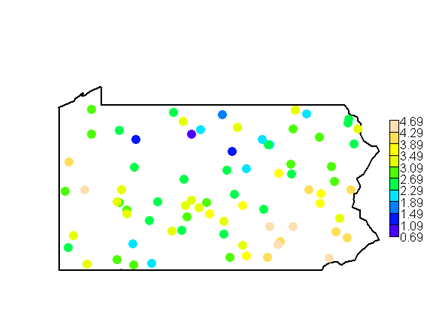
\includegraphics[height=2.75in]{figs/PA1}
\end{center}
\caption{Needs a caption}
\label{fig.PA1}
\end{figure}

We do have a measure of forest cover in the vicinity of each point which is contained in the data set (``habitat''). This was derived from a larger GIS coverage of the state (provided in the data file ``pahabdata'') which can be plotted using the spatial.plot function using the following commands
\begin{verbatim}
> map('state',regions="penn",lwd=2)
> spatial.plot(pahabdata[,2:3],pahabdata[,"dfor"],cx=2)
> map('state',regions="penn",lwd=2,add=TRUE)
\end{verbatim}


\begin{figure}
\begin{center}
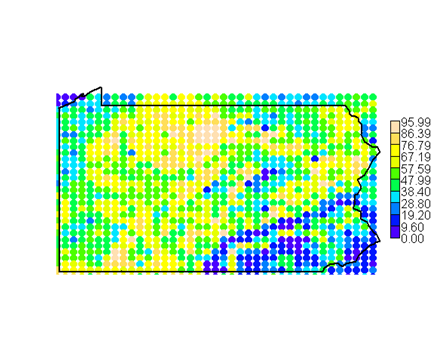
\includegraphics[height=2.75in]{figs/PA2}
\end{center}
\caption{Needs a caption}
\label{fig.PA21}
\end{figure}


We see a prominent pattern that indicates high forest coverage in the
central part of the state and low forest cover in the SE.  Inspecting
the previous figure of log-counts suggests a relationship between
counts and forest cover which is not surprising.

\subsection{Doing it in WinBUGS}
Here we demonstrate how to fit a Poisson GLM in WinBUGS using the covariate $x(i) =$ forest cover. It is advisable that $x(i)$ be standardized in most cases as this will improve mixing of the Markov chains. Recall that the data we have stored include a standardized covariate (forest cover) and so we don't have to worry about that here.  To read the BBS data into R and get things set up for WinBUGS we issue the following commands: 
\begin{verbatim}
data<-read.csv("pa-bbsdovedata-all.csv")
y<-data[,29]  # pick out 1990
notna<-!is.na(y)
y<-y[notna]
habitat<-data[notna,4]
library("R2WinBUGS")
data <- list ( "y","M","habitat")
\end{verbatim}
Now we write out the Poisson model specification in WinBUGS pseudo-code, provide initial values, identify parameters to be monitored and then execute WinBUGS:
\begin{verbatim}
cat("
model {
    for (i in 1:M){
      y[i]~dpois(lam[i])
      log(lam[i])<- beta0+beta1*habitat[i]
     }
 beta0~dunif(-5,5)
 beta1~dunif(-5,5)
}
",file="PoissonGLM.txt")

inits <- function()  list ( beta0=rnorm(1),beta1=rnorm(1))
parameters <- c("beta0","beta1")
out<-bugs (data, inits, parameters, "PoissonGLM.txt", n.thin=2, n.chains=2, n.burnin=2000,n.iter=6000,debug=TRUE,working.dir=getwd())
\end{verbatim}

{\bf Remarks:} (1) Note the close correspondence in how the model is specified here compared with the normal regression model previously. As an exercise you should discuss the specific differences between the BUGS model specifications for the normal and Poisson models.
\begin{verbatim}
> print(out,digits=3)
Inference for Bugs model at 
``PoissonGLM.txt'', fit using WinBUGS,
 2 chains, each with 4000 iterations (first 1000 discarded), n.thin = 2
 n.sims = 3000 iterations saved
             mean     sd     2.5%      25%      50%      75%    97.5%  Rhat n.eff
beta0       3.151  0.025    3.102    3.135    3.151    3.168    3.199 1.001  2300
beta1      -0.498  0.021   -0.539   -0.512   -0.498   -0.484   -0.457 1.001  3000
fit       869.930 19.856  835.500  855.700  868.600  881.900  913.602 1.002  1600
fitnew     76.709 12.519   54.098   68.107   76.215   84.510  102.602 1.001  3000
deviance 1116.605  2.014 1115.000 1115.000 1116.000 1117.000 1122.000
1.001  3000
\end{verbatim}


We might wonder whether this model provides an adequate fit to our data.  To evaluate that, we used a Bayesian p-value analysis with fit statistic based on the Freeman-Tukey residual by replacing the model specification above with this:

\begin{verbatim}
cat("
model {
    for (i in 1:M){
      y[i]~dpois(lam[i])
      log(lam[i])<- beta0+beta1*habitat[i]
      d[i]<-  pow(pow(y[i],0.5)-pow(lam[i],0.5),2)   #

      ynew[i]~dpois(lam[i])
      dnew[i]<-pow( pow(ynew[i],0.5)-pow(lam[i],0.5),2)

     }
 fit<-sum(d[])
 fitnew<-sum(dnew[])
 beta0~dunif(-5,5)
 beta1~dunif(-5,5)
}


",file="PoissonGLM.txt")
\end{verbatim}
The Bayesian p-value is the proportion of times $fitnew > fit$ which, for this data set, is 0, which was 1.0 in this case (calculation omitted). This suggests that the basic Poisson model does not fit well. 


\subsection{ Constructing your own MCMC algorithm}

It will be helpful for people to suffer through a couple examples building a custom MCMC algorithm. So, here, we build a basic one for the Poisson regression model using a Metropolis-within-Gibbs approach. First, we will assume that the two parameters have diffuse normal priors, say $[\alpha] = norm(0,100)$ and $[\beta]=norm(0,100)$.  We need to collect the relevant elements of the model which are the likelihood $[y|\alpha,\beta] = prod_{i} [y[i]|\alpha\beta] $ which is, mathematically, the product of the Poisson pmf evaluated at $y[i]$, given particular values of $\beta0$ and $\beta1$. The priors are $[\alpha]$ and $[\beta]$. We identify the full conditionals which are $[\alpha|\beta, y]$ and $[\beta|\alpha,y]$.  We use the all-purpose rule for constructing full conditionals to discover that:
\[
 [\alpha|\beta,y] propto [y|\alpha,\beta][\alpha] 
\]
\[
 [\beta|\alpha,y] propto [y|\alpha,\beta][\beta]
\]
Remember we could replace the ``propto'' with ``equals'' if we simply put $[y|\beta]$ or $[y|\alpha]$ in the denominator. But, in general, $[y|\alpha]$ or $[y|\beta]$ will be quite a pain to compute and, more importantly, it is a constant as far as the operative parameter (beta or alpha, respectively) goes so we can just as well ignore it because, recall, the MH acceptance probability will be the ratio of the ful-conditional evaluated at a candidate draw to that evaluated at the current draw. So, the denominator required to change $\propto$ to $=$ winds up canceling from the MH acceptance probability.  Here we will use the random walk candidate generator.  The ``Metropolis within Gibbs'' algorithm for a Poisson regression is remarkably simple:

%% Kimmy: test this R code out below and see what happens!

\begin{verbatim}I would break this code up into more lines and have objects called ``prior'' and ``prior.candidate'' and ``lambda'' and ``likelihood.candidate''. Annoying stuff that will make it easier for people to understand. Also, remind people that $lik*prior = exp(log(like)+log(prior))$. Lots of people have been running around in the woods for years with traps, and have forgotten math.

You could also mention that this is a random walk M-H. It would help lots of people out to see a non-symmetric proposal distribution, and the extra step needed to account for it.

# put random number seed here
out<-matrix(NA,nrow=1000,ncol=2)   # matrix to store the output
beta0<- -1                         # starting values
beta1<- -.8

# begin the MCMC loop ; do 1000 iterations
for(i in 1:1000){

# update the beta0 parameter
lik.curr<- sum(log(dpois(y,exp(beta0+beta1*habitat)))) 
prior.curr<- log(dnorm(beta0,0,100))
beta0c<-rnorm(1,beta0,.25)         # generate candidate
lik.cand<- sum(log(dpois(y,exp(beta0c+beta1*habitat))))
prior.cand<- log(dnorm(beta0c,0,100))
if(runif(1)< exp(lik.cand+prior.cand-lik.curr-prior.curr)) beta0<-beta0c

# update the beta1 parameter
lik.curr<- sum(log(dpois(y,exp(beta0+beta1*habitat)))) 
prior.curr<- log(dnorm(beta1,0,100))
beta1c<-rnorm(1,beta1,.25)
lik.cand<- sum(log(dpois(y,exp(beta0+beta1c*habitat)))) 
prior.cand<- log(dnorm(beta1c,0,100))
if(runif(1)< exp(lik.cand+prior.cand-lik.curr-prior.curr)) beta1<-beta1c
out[i,]<-c(beta0,beta1)             # save the current values
}
\end{verbatim}


\begin{figure}
\begin{center}
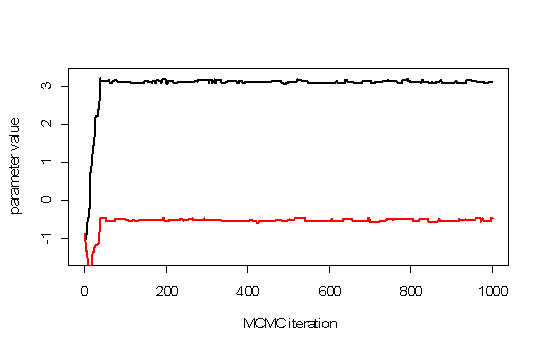
\includegraphics[height=2.75in]{figs/MCMC1}
\end{center}
\caption{Needs a caption}
\label{fig.MCMC1}
\end{figure}


Look at the output (beta0 in red, beta1 in black). You might not like the appearance of this output too much but a couple of things are evident: The Markov chains clearly stabilize - ``converge'' --  after about 100 iterations. They also appear to mix very slowly, although this is not so clear given the scale of the y-axis.
 

We decreased the variance for candidate generating distribution and
re-ran the MCMC algorithm producing the history plots below. We see
that the burn-in takes longer but it seems to mix better.


Fig. XYZ shows a longer MCMC run (10,000 total iterations) for beta1
based on discarding the first 400 samples as burn-in. The ``grassy''
look of the MCMC history is diagnostic of Markov chains that are
well-mixing.

\begin{figure}
\begin{center}
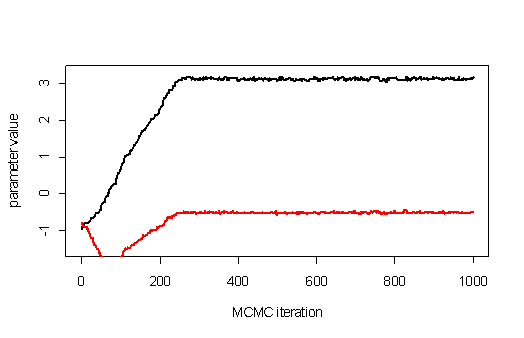
\includegraphics[height=2.75in]{figs/MCMC2}
\end{center}
\caption{Needs a caption}
\label{fig.MCMC2}
\end{figure}


\begin{figure}
\begin{center}
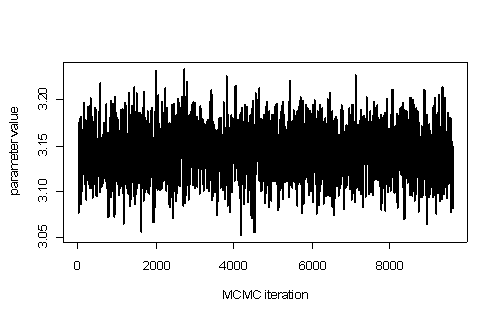
\includegraphics[height=2.75in]{figs/MCMC3}
\end{center}
\caption{Needs a caption}
\label{fig.MCMC3}
\end{figure}

{\bf Remarks:} We used a specific set of starting values for these
simulations. It should be clear that starting values closer to the
mass of the posterior distribution might cause burn-in to occur
faster. As an exercise, evaluate that.  (2) Clearly the influence of
the proposal variance term is important. Small values lead to much
better mixing but it should be noted that values that are too small
will lead to very slow mixing. We saw that values that were too large
tended to get the parameters stuck in one spot. This suggests there is
an optimal value of the Metropolis-Hastings tuning
parameter\footnote{Defined previously?}. As an exercise you should
find that optimal value. (3) For the flat normal prior distributions
here we could leave the prior contribution out of the full conditional
evaluation since it is ``locally constant''. Note also that we have
used a different prior than in our WinBUGS model specification. As an
exercise, evaluate whether this seems to affect the result.

\section{Poisson GLM with Random Effects}

What we will be doing in most of this book is dealing with random effects in GLM-like models - models that are usually referred to as generalized linear mixed models (GLMMs).

{\bf The Log-Normal mixture:} The classical situation involves a GLM with a normally distributed random effect. The linear predictor of the Poisson model is extended simply by adding a noise term, say:
\[
 	log(\lambda(i)) = \alpha  + \beta*x(i) + \eta[i]
\]
where $\eta[i]~normal(0,\sigma2)$.  A natural alternative is to have $exp(\eta[i])/\sim\gamma(a,b)$ which would correspond to a negative binomial kind of over-dispersion whereas the normal noise has a different mean/variance relationship (the interested reader should work that out).   Choosing between such possibilities is not a topic we will get into here because it doesn't seem possible to provide general guidance on it. Anyhow, it is really amazingly simple to express this model in WinBUGS and have WinBUGS draw samples from the posterior distribution using the following code for the BBS dove counts: 
\begin{verbatim}
data<-read.csv("pa-bbsdovedata-all.csv")
locs<-data[,2:3]
habitat<-data[,4]
y<-data[,29]
notna<-!is.na(y)  # to remove missing values
y<-y[notna]
locs<-locs[notna,]
habitat<-habitat[notna]
M<-length(y)

cat("
model {
            for (i in 1:M){
               y[i]~dpois(lam[i])
               log(lam[i])<- beta0+beta1*habitat[i] + eta[i]
               eta[i] ~ dnorm(0,tau)
               }
 beta0~dunif(-5,5)
 beta1~dunif(-5,5)
 sigma~dunif(0,10)
 tau<-1/(sigma*sigma)
}
\end{verbatim}
I have removed the final several R commands which package up the data and execute WinBUGS as those commands are largely redundant with the previous demo.  The summary results are:
\begin{verbatim}
> print(out,digits=3)
Inference for Bugs model at "model.txt", fit using WinBUGS,
 2 chains, each with 5000 iterations (first 1000 discarded), n.thin = 2
 n.sims = 4000 iterations saved
            mean     sd    2.5%     25%     50%     75%   97.5%  Rhat n.eff
beta0      2.967  0.076   2.817   2.915   2.969   3.020   3.111 1.006   430
beta1     -0.518  0.073  -0.657  -0.566  -0.517  -0.470  -0.374 1.008  4000
sigma      0.598  0.059   0.491   0.556   0.594   0.634   0.725 1.004   640
tau        2.883  0.569   1.904   2.489   2.836   3.233   4.149 1.004   640
fit       19.885  3.190  14.119  17.670  19.705  21.902  26.610 1.001  4000
fitnew    20.043  3.422  14.100  17.630  19.770  22.292  27.360 1.001  4000
deviance 446.255 12.290 424.000 437.700 445.600 454.100 472.302 1.001  4000

For each parameter, n.eff is a crude measure of effective sample size,
and Rhat is the potential scale reduction factor (at convergence, Rhat=1).

DIC info (using the rule, pD = Dbar-Dhat)
pD = 66.0 and DIC = 512.2
DIC is an estimate of expected predictive error (lower deviance is better).
> 

\end{verbatim}

The Bayesian p-value for this model is
\begin{verbatim}
> mean(out$sims.list$fit>out$sims.list$fitnew)
[1] 0.473
>
\end{verbatim}
indicating a pretty good fit. Given the site-level random effect, it
would be surprising for this model to not fit! One thing we notice is
that the posterior standard deviations of the regression parameters
are much higher, a result of the excess variation. (we would also
notice much less precise predictions of hypothetical new
observations).


\section{Binomial GLMs}

Another class of statistical models that are very important in ecology are binomial models. We use binomial models for count data whenever the observations are counts or frequencies and it is natural to condition on a ``sample size'' - the maximum frequency possible in a sample, say $K$ (i.e., $K$ is known). The random variable, $y/le K$, is then the frequency of occurrences out of $K$. The parameter of the binomial models is $p$, often called ``success probability'' which is related to the expected value of $y$ by $E[y] = pK$. Binomial GLMs or binomial regression models are often referred to as logistic regression, but that term really only applies when the logistic link is used to model the relationship between $p$ and covariates (see below).

One of the most typical Binomial GLMs occurs when the sample size
equals 1 and the outcome, $y$, is ``presence'' ($y=1$) or ``absence''
($y=0$) of a species. This is a classical ``species distribution''
modeling situation. A special situation occurs when presence/absence
is observed with error \citep{mackenzie_etal:2002,
  mackenzie_etal:2006, kery_etal:2010}. In that case, $K>1$ samples
are usually required in order to estimate model parameters
effectively. In standard binomial regression problems the sample size
is fixed by design but interesting models also arise when the sample
size is itself a random variable. These are the N-mixture models
\citep{royle:2004, kery_etal:2005, royle_dorazio:2008, kery:2010}
ch. 22) and related models (in this case, $N$ being the sample size
which we labeled K above). This is actually a little bit confusing
because the binomial index is usually referred to as ``sample size''
but in this context N is actually a ``population size''.  A useful
situation in which the binomial sample size is ``fixed'' is closed
population capture-recapture models in which a population of
individuals is sampled $K$ times.  The number of times each individual
is encountered is a binomial outcome with parameter - encounter
probability - $p$, based on a sample of size $K$.  We consider such
models in the following chapter.


\subsection{Binomial regression}

 In binomial models, covariates are modeled on a suitable transformation (the link function) of the binomial success probability, $p$.  Let  $x_{i}$ denote some measured covariate for sample unit $i$ and let $p_{i}$ be the success probability for unit i.  The standard choice is the ``logit'' link function which is:
\[
log(p[i]/(1-p[i])) = \alpha + \beta*x[i]
\]
with inverse ``expit''
\[
p[i] = expit(\alpha + \beta*x[i]) = exp(\alpha + \beta*x[i])/(1 + exp(\alpha + \beta*x[i])) 
\]
There are many other possible link functions. However, ecologists seem
to blindly adopt the logit link function without question to such an
extent that you are likely to be questioned by referees and associate
editors if you use some alternative link (unless you are doing species
distribution modeling, in which case any explicit link function will
be questioned by some referees).  We sometimes use the ``complementary
log-log'' (= ``cloglog'') link function in ecological applications
because it can often be justified based on subject-matter
considerations (\citet{royle_dorazio:2008}; section XYZ) or natural
scaling relationships germane to the problem.  For example, the
cloglog link arises as the ``probability of a count greater than 0''
under a Poisson model. That is, $\Pr(y>0) = 1-exp(- \lambda)$ in which case
\[
cloglog(p) =log(- log(1-p)) = log(\lambda)
\]
So that if you have covariates in your linear predictor for $E[y]$ under a Poisson model then they are linear on the complementary log-log link of p. We will use the cloglog link in some analyses of SCR models in Chapter 4 and elsewhere.  

A natural situation in which the cloglog link arises is modeling occupancy in which $N \sim Poisson(A*\lambda)$ and you have site area, A, measured for every sample. In this case the probability that the site is occupied, psi, is related to area on the cloglog scale. i.e.,
\[
 cloglog(\psi) = log(A) + log(\lambda).
\]
There seems to be perennial debate over whether site area should be a
covariate on ``detection'' or ``occupancy'' and the above argument
suggests the latter.


\subsection{ Example: Waterfowl Banding Data}

It would be easy to consider a standard ``distribution modeling''
application where $K=1$ and the outcome is occurrence ($y=1$) or not
($y=0$) of some species. Such examples abound in books (e.g.,
\citet{royle_dorazio:2008}, ch. 3; \citet{kery:2010}, chapter 21 XYZ?;
\citet{kery_schaub:2011}, chapter XYZ) and in the literature (see
\citet{kery_etal:2010}; \citet{kery_etal:2010} XYZ).  Instead, we will consider an example involving band returns of waterfowl which were analyzed by Royle and Dubovsky (200X)\footnote{not happy about this example. Anyone got a better one?}.  

For these data, $y[i]$ is the number of waterfowl bands recovered out of $B[i]$ birds banded at some location $s[i]$. In this case $B[i]$ is fixed. Thinking about recovery rate as being proportional to harvest rate, we wanted to explore geographic gradients in recovery rate resulting from variability in harvest pressure experienced by populations depending on their migration ecology. As such, we fit a basic binomial GLM with a linear response to geographic coordinates (including an interaction term). The data are provided on the web supplement along with an R script to do the post-processing. Here we just provide the part of the script for creating the model and calling WinBUGS:

\begin{verbatim}
sink("model.txt")
cat("
model {
 for(t in 1:5){
    for (i in 1:nobs){
       m[i,t] ~ dbin(p[i,t], R[i,t])
       logit(p[i,t]) <- alpha0[t] + alpha1*X[i,1] + alpha2*X[i,2] + alpha3*X[i,1]*X[i,2]
     }
}
	alpha1~dnorm(0,.001)
	alpha2~dnorm(0,.001)
	alpha3~dnorm(0,.001)
	for(t in 1:5){
 	alpha0[t] ~ dnorm(0,.001)  
 }
}
",fill=TRUE)
sink()

data <- list('R', 'm', 'nobs','X')
inits <- 	function(){
list(alpha0=rnorm(5),alpha1=0,alpha2=0,alpha3=0)
}
parms <- list('alpha0','alpha1','alpha2','alpha3')
out <- bugs(data,inits, parms,"model.txt",n.chains=3,
 					n.iter=2000,n.burnin=1000,
					n.thin=2, debug=TRUE)
\end{verbatim}

Posterior summaries of model parameters are as follows:

\begin{verbatim}
Inference for Bugs model at "model.txt", fit using WinBUGS,
 3 chains, each with 2000 iterations (first 1000 discarded), n.thin = 2
 n.sims = 1500 iterations saved
              mean    sd     2.5%      25%      50%      75%    97.5%  Rhat n.eff
alpha0[1]   -2.346 0.036   -2.417   -2.370   -2.346   -2.323   -2.277 1.001  1500
alpha0[2]   -2.356 0.032   -2.420   -2.379   -2.356   -2.335   -2.292 1.001  1500
alpha0[3]   -2.220 0.035   -2.291   -2.244   -2.219   -2.197   -2.153 1.001  1500
alpha0[4]   -2.144 0.039   -2.225   -2.169   -2.143   -2.116   -2.068 1.000  1500
alpha0[5]   -1.925 0.034   -1.990   -1.949   -1.924   -1.901   -1.856 1.004   570
alpha1      -0.023 0.003   -0.028   -0.025   -0.023   -0.022   -0.018 1.001  1500
alpha2       0.020 0.006    0.009    0.016    0.020    0.024    0.031 1.001  1500
alpha3       0.000 0.001   -0.002   -0.001    0.000    0.000    0.002 1.001  1500
deviance  1716.001 4.091 1710.000 1713.000 1715.000 1718.000 1726.000 1.001  1500

For each parameter, n.eff is a crude measure of effective sample size,
and Rhat is the potential scale reduction factor (at convergence, Rhat=1).

DIC info (using the rule, pD = Dbar-Dhat)
pD = 7.9 and DIC = 1723.9
DIC is an estimate of expected predictive error (lower deviance is better).
\end{verbatim}

The basic result suggests a negative east-west gradient and a positive south to north gradient but no interaction. A map of the response surface is given below. We could use DIC to do some model selection - i.e., try models without the interaction term, or models with a quadratic term, or with a constant intercept, etc., but we don't pursue that here. We did an MCMC run where we saved the binomial parameter p and computed the Bayesian p-value [double use of ``p'' here is confusing!] using a fit statistic based on the Freeman-Tukey statistic (see Section XXX above). The result indicates that the linear response surface model does not provide an adequate fit of the data. The reader should contemplate whether this invalidates the basic interpretation of the result.


\begin{figure}
\begin{center}
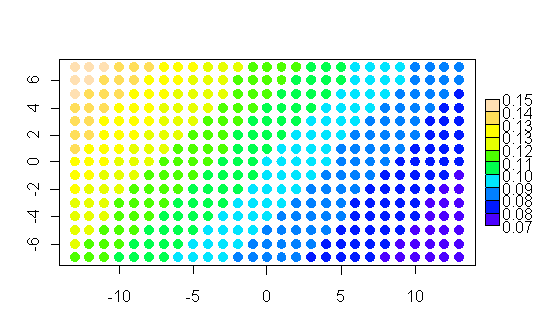
\includegraphics[height=2.75in]{figs/responsesurface}
\end{center}
\caption{Needs a caption}
\label{fig.responsesurface}
\end{figure}

\section{ Summary and Outlook}


GLMs and GLMMs are the most useful statistical methods in all of ecology. The principles and procedures underlying these methods are relevant to nearly all modeling and analysis problems in every branch of ecology. Moreover, understanding how to analyze these models is crucial in a huge number of diverse problems. If you understand and can conduct classical likelihood and Bayesian analysis of Poisson and binomial GLM(M)s, then you will be successful analyzing and understanding more complex classes of models that arise.We will see shortly that spatial capture-recapture models are just a type of GLMM (i.e., a GLM with a random effect) and thus having a basic understanding of the conceptual origins and formulation of GLMs and their analysis is extremely useful. We note that GLMs are routinely analyzed by likelihood methods but we have focused on Bayesian analysis here in order to develop the tools that are less familiar to most ecologists.  In particular, Bayesian analysis of GLMs with random effects (i.e., GLMMs) is relatively straightforward because the models are easy to analyze conditional on the random effect, using methods of MCMC.  Thus, we will often analyze SCR models in later chapters by MCMC, explicitly adopting a Bayesian inference framework.

In that regard, BUGS engines are enormously useful because they provides a straightforward way to carry out analyses by MCMC by just describing the model, and not having to worry about how to actually build MCMC algorithms.  That said, the BUGS language is more important than just to the extent that it enables one to do MCMC - it is useful as a modeling tool because it fosters understanding, in the sense that it forces you to become intimate with your model. You have to write down all of the probability assumptions, the relationships between observations and latent variables and parameters. This is really a great learning paradigm that you can grow with. Skills gained in Bayesian analysis of the GLMMs covered in this chapter will be directly transferrable and useful for the SCR models addressed subsequently. Before getting to that, however, it will be useful to talk about more basic, conventional closed population capture-recapture models and these are the topic of the next Chapter. 

%\chapter{Essentials of Statistical Inference} \label{chapt.stats}

%\chapter{Occupancy and Occurrence Models} \label{chapt.occ}
%\input{Chapter3.tex}



\markboth{Bibliography}{Bibliography}

\bibliographystyle{asa}
\bibliography{AndyRefs_alphabetized}

%%\bibliography{AndyRefs.bib}

%\bibliographystyle{alpha}
%\bibliography{mybib}

\markboth{Index}{Index}

%\printindex

%\input{Allbook-main.ind}


\end{document}
















































